\documentclass[9pt,twocolumn,twoside]{gsajnl}
% Use the documentclass option 'lineno' to view line numbers
% Package imports
\usepackage{gensymb}
\usepackage[labelformat=simple]{subcaption}
\renewcommand*{\thesubfigure}{\Alph{subfigure}}
\usepackage{tabularx, multirow}
\usepackage{makecell}
\hypersetup{draft}

\usepackage{siunitx}
\sisetup{output-exponent-marker=\ensuremath{\mathrm{e}}}


%\usepackage[dvipsnames]{xcolor}
%\usepackage{enumitem}
%\newcommand{\method}[1]{\qquad Method #1}
\usepackage{soul}
\usepackage{xspace}
\newcommand{\indep}{\rotatebox[origin=c]{90}{$\models$}}
\newcommand{\eg}{\emph{e.g.}\xspace}
\newcommand{\ie}{\emph{i.e.}\xspace}
\newcommand{\T}{^\mathrm{T}}
\newcommand{\bbeta}{\boldsymbol{\beta}}
\newcommand{\blup}{\widetilde{\bbeta}}
\newcommand{\bzero}{\mathbf{0}}
\newcommand{\bI}{\mathbf{I}}
\newcommand{\bx}{\mathbf{x}}
\newcommand{\by}{\mathbf{y}}
\newcommand{\tausq}{\tau^{2}}
\newcommand{\qtl}{\widehat{h^{2}}_{\text{QTL}}}

\newcommand{\WV}[2]{\textcolor{red}{#1\footnote{\textcolor{red}{WV: #2}}}}
\newcommand{\WVinline}[1]{\textcolor{red}{#1}}
\newcommand{\WVst}[1]{\textcolor{red}{\st{#1}}}
\newcommand{\reply}{\ensuremath{\hookrightarrow}\xspace}
\newcommand{\addheadline}{\subsubsection{\WVinline{[Add headline]}\xspace}}

\newcommand{\GK}[2]{\textcolor{teal}{#1\footnote{\textcolor{teal}{GK: #2}}}}
\newcommand{\GKinline}[1]{\textcolor{teal}{#1}}


\articletype{inv} % article type
% {inv} Investigation 
% {gs} Genomic Selection
% {goi} Genetics of Immunity 
% {gos} Genetics of Sex 
% {mp} Multiparental Populations

% scrub Genetics journal info -- for submission and biorxiv
\fancypagestyle{firststyle}{}
\renewcommand{\firstpagefootnote}{\blfootnote{Manuscript compiled: \today}}

%\title{Tissue-specific QTL analysis of gene expression and chromatin accessibility in the Collaborative Cross mouse population}
%\title{Chromatin-mediated gene expression within three tissues using the Collaborative Cross mouse resource}

\title{Integrative QTL analysis of gene expression and chromatin accessibility identifies multi-tissue patterns of genetic regulation}

\author[$\ast$,$\dagger$,$\ddagger$,$\ast\ast\ast$]{Gregory R. Keele}
\author[$\ast$,$\dagger$,$\ddagger$,$\dagger\dagger\dagger$]{Bryan C. Quach}
\author[$\ddagger$]{Jennifer W. Israel}
\author[$\ddagger\ddagger$]{Yihui Zhou}
\author[$\S\S$]{Grace A. Chappell}
\author[$\S\S$]{Lauren Lewis}
\author[$\dagger\dagger$]{Alexias Safi}
\author[$\ddagger$]{Jeremy M. Simon}
\author[$\ddagger$]{Paul Cotney}
\author[$\dagger\dagger$]{Gregory E. Crawford}
\author[$\ddagger\ddagger$]{Fred A. Wright}
\author[$\ddagger$,$\ast\ast$]{William Valdar}
\author[$\S\S$,1]{Ivan Rusyn}
\author[$\ddagger$,$\S$,$\ast\ast$,1]{Terrence S. Furey}

\affil[$\ast$]{Authors contributed equally}
\affil[$\dagger$]{Curriculum in Bioinformatics and Computational Biology}
\affil[$\ddagger$]{Department of Genetics}
\affil[$\S$]{Department of Biology}
\affil[$\ast\ast$]{Lineberger Comprehensive Cancer Center, University of North Carolina at Chapel Hill}
\affil[$\dagger\dagger$]{Department of Pediatrics, Center for Genomic and Computational Biology, Duke University, Durham, NC}
\affil[$\ddagger\ddagger$]{Departments of Statistics and Biological Sciences, North Carolina State University, Raleigh, NC}
\affil[$\S\S$]{Department of Veterinary Integrative Biosciences, Texas A\&M University, College Station, TX}
\affil[$\ast\ast\ast$]{The Jackson Laboratory, Bar Harbor, ME}
\affil[$\dagger\dagger\dagger$]{Center for Omics Discovery and Epidemiology, Research Triangle Institute (RTI) International\hspace{17cm} ORCID IDs: 
0000-0002-1843-7900 (G.R.K.), 0000-0002-1094-3104 (B.C.Q.), 0000-0003-3906-1663 (J.M.S.), 0000-0002-2419-0430 (W.V.)}

\keywords{multiparental populations (MPP), Collaborative Cross (CC), Diversity Outbred (DO), mediation, genome-wide association (GWA)}

\runningtitle{Integrative QTL analysis across multiple tissues in the Collaborative Cross} % For use in the footer 

\runningauthor{Keele \textit{et al.}}

\begin{abstract}

\WVinline{MY EDITED ABSTRACT:} 
The transcriptional profiles of genes across tissues are modulated by, among other things, genetic variation and chromatin accessibility. \WVinline{The interplay of these factors, however, is poorly understood. [TERRY F to edit as appropriate.]}
Here we characterize expression and chromatin state dynamics across three tissues---liver, lung, and kidney---in 47 strains of the 
Collaborative Cross (CC) mouse population, paying particular attention to the regulation of these dynamics by expression quantitative trait loci (eQTL) and chromatin QTL (cQTL). 
QTL whose allelic effects were common across tissues were detected for 1,101 genes and 133 chromatin regions.
Also detected were tissue-specific QTL, for both genes and chromatin, including a local eQTL for \textit{Pik3c2g} detected in all three tissues but with distinct allelic effects.
Leveraging the overlapping measurement of gene expression and chromatin accessibility on the same mice from multiple tissues, we used mediation analysis to identify chromatin and gene expression intermediates of eQTL effects. 
Based on QTL and mediation analyses over multiple tissues, we propose a causal model for the distal genetic regulation of \textit{Akr1e1}, a gene involved in glycogen metabolism, through a zinc finger protein and chromatin intermediates.
This analysis demonstrates the complexity of transcriptional and chromatin dynamics and their regulation over multiple tissues, as well as the value of the CC and related genetic resource populations for identifying specific regulatory mechanisms in biological data.

\WVinline{OLD ABSTRACT:}
Many factors such as genetic variation and chromatin accessibility modulate the transcriptional profiles of genes across tissues.
 We analyzed gene transcript and chromatin accessibility levels from liver, lung, and kidney tissues for 47 strains of the Collaborative Cross (CC) mouse population to characterize expression and chromatin state dynamics across tissues, with particular attention paid to their genetic regulation through the identification of expression quantitative trait loci (eQTL) and chromatin QTL (cQTL). We detected 1,101 genes and 133 chromatin regions that possessed QTL with correlated founder haplotype effects across multiple tissues. Tissue-specific QTL were also detected genes and chromatin, including \textit{Pik3c2g} with distinct local-eQTL observed in all three tissues. Leveraging the overlapping measurement of gene expression and chromatin accessibility on the same mice from multiple tissues, we used mediation analysis to identify chromatin and gene expression intermediates of eQTL effects. Based on QTL and mediation analyses over multiple tissues, we propose a causal model for the distal genetic regulation of \textit{Akr1e1}, a gene involved in glycogen metabolism, through a zinc finger protein and chromatin intermediates. This analysis demonstrates the complexity of transcriptional and chromatin dynamics and their regulation over multiple tissues, as well as the value of the CC and related genetic resource populations for identifying specific regulatory mechanisms in biological data.

\end{abstract}

\setboolean{displaycopyright}{true}

\begin{document}

\maketitle
\thispagestyle{firststyle}
%\marginmark
\firstpagefootnote
\correspondingauthoraffiliation{Corresponding authors: 4458 TAMU, Texas A \& M University, College Station, TX 77843. 

E-mail: irusyn@tamu.edu

120 Mason Farm Rd., Genetic Medicine Bldg., Suite 5113, University of North Carolina, Chapel Hill, NC 27599. 

E-mail: tsfurey@email.unc.edu}
\vspace{-11pt}%

\linenumbers
%%%%%%%%%% Introduction
Determining the mechanisms by which genetic variants drive molecular, cellular, and physiological phenotypes has proved to be challenging \citep{Schadt2009}. These mechanisms can be informed by genome-wide experiments that provide data on variations in molecular and cellular states in genotyped individuals, but most examples of such data are largely observational, due in part to constraints of specific populations (\eg, humans), the limitations of existing experimental technologies, and the challenge of coordinating large numbers of experiments with multiple levels of data \citep{Schaid2018}. 
One approach to shed light on these dynamics is to pair complementary datasets from the same individuals and perform statistical mediation analysis (\eg \citealt{Baron1986, Mackinnon2007}), an increasingly tool in genomics \citep{Richmond2016}. These analyses can identify putative causal relationships rather than correlational interactions, providing meaningful and actionable targets in terms of downstream applications in areas such as medicine and agriculture.

%Integrative analyses can inform upon the regulation of fundamental biological processes, such as through the combined assessment of gene transcription and gene regulation data. 
%\cite{Degner2012} correlated chromatin accessibility quantitative trait loci (cQTL) with gene expression QTL (eQTL) in human lymphoblastoid cell lines, to suggest how some genetic variants modulated transcription though chromatin state. 
%\cite{Battle2014} investigated the regulation of gene expression in 922 humans, using eQTL and allele specific expression QTL to assess evidence for genes proximal to distal-eQTL behaving as mediators to distal-eQTL target genes. 
In human data, co-occurence of QTL across various multi-omic data has been used to assess the potential for related and connected biological processes; examples include gene expression with chromatin accessibility \citep{Degner2012}, regulatory elements \citep{Pai2015},  and ribosome occupancy and protein \citep{Battle2015, Yang2017}.
More formal integration through statistical mediation analyses have also been used to investigate relationships between levels of human biological data, \eg, distal-eQTL with local gene expression \citep{Battle2014}, and eQTL with regulatory elements \citep{Alasoo2017, Roytman2018, Wu2018}.
%\cite{Pai2015} localized eQTL to genomic regulatory elements in human lymphoblastoid cell line data to infer the mode of action of the QTL. \cite{Alasoo2017} further elucidated the roles of eQTL within regulatory elements by testing the effect of enhancer sequence modifications. \cite{Roytman2018} propose the use of probabilistic mediation models, finding they perform better to detect relationships between histone modification QTL (hQTL) and eQTL in comparison to simple QTL overlap in data from 112 humans. \cite{Wu2018} use mediation to tease apart the relationships among DNA methylation sites, gene expression, and complex traits. 
%\cite{Battle2015} detected the co-localization of eQTL, ribosome occupancy QTL (rQTL), and protein abundance (pQTL), observing significant overlap and a potential buffering of rQTL effects on protein levels.

%\WV{Despite these successes, using data from human populations for genotype-phenotype analyses is challenging, in part due to an inability to tightly control experimental conditions and genetic backgrounds to reproducibly and unambiguously detect casual linkages.}{Needs rewording.} 
Though genetic association studies of human populations have been highly successful \citep{Visscher2017}, animal models allow for more deliberate control of the additional sources of variation, including experimental conditions and genetic backgrounds, and thereby provide a potentially powerful basis for detecting associations and even causal linkages.
To aid in this effort, genetically-diverse mouse population resources have been established, including the Collaborative Cross (CC) \citep{Churchill2004,Hall2012,Srivastava2017} and the Diversity Outbred (DO) mice \citep{Churchill2012}. The CC and the DO are derived from the same eight founder strains: (short names in parentheses): A/J (AJ), C57BL/6J (B6), 129S1/SvImJ (129), NOD/ShiLtJ (NOD), NZO/H1LtJ (NZO), CAST/EiJ (CAST), PWK/PhJ (PWK), and WSB/EiJ (WSB). The CC are recombinant inbred strains and therefore replicable across and within studies; the DO are largely heterozygous, outbred animals, bred with a random mating strategy that seeks to maximize diversity. 

A genome-wide mediation approach in 192 DO mice was used in \citet{Chick2016} to link transcriptional and post-translational regulation of protein levels; they also used the CC to confirm results by showing that estimates of founder haplotype effects from each of the related populations corresponded. More recently, mediation analysis was used to connect chromatin accessibility with gene expression in embryonic stem cells derived from DO mice \citep{Skelly2019}.

Here we use a sample composed of a single male mouse from 47 strains of the CC to investigate tissue-specific dynamics between gene expression and  chromatin accessibility, as determined by Assay for Transposase Accessible Chromatin sequencing (ATAC-seq), in lung, liver, and kidney tissues. We detect QTL underlying gene expression and chromatin accessibility variation across the strains, and assess the support for mediation of the effect of eQTL through chromatin accessibility using a novel implementation of methods adapted from \cite{Chick2016}. Additionally, we detect gene mediators of distal-eQTL. 
%We identify and characterize examples of strong mediation, as well as co-localizing but independent eQTL and cQTL. 
These findings demonstrate the experimental power of the CC for integrative analysis of multi-omic data to determine genetically-driven phenotype variation, despite limited sample size, and provide support for continued use of the CC in larger experiments going forward.

%%%%%%%%%% Methods
\section{Materials and Methods}
\label{sec:materials:methods}

\begin{figure*}[htbp]
\renewcommand{\familydefault}{\sfdefault}\normalfont
\centering
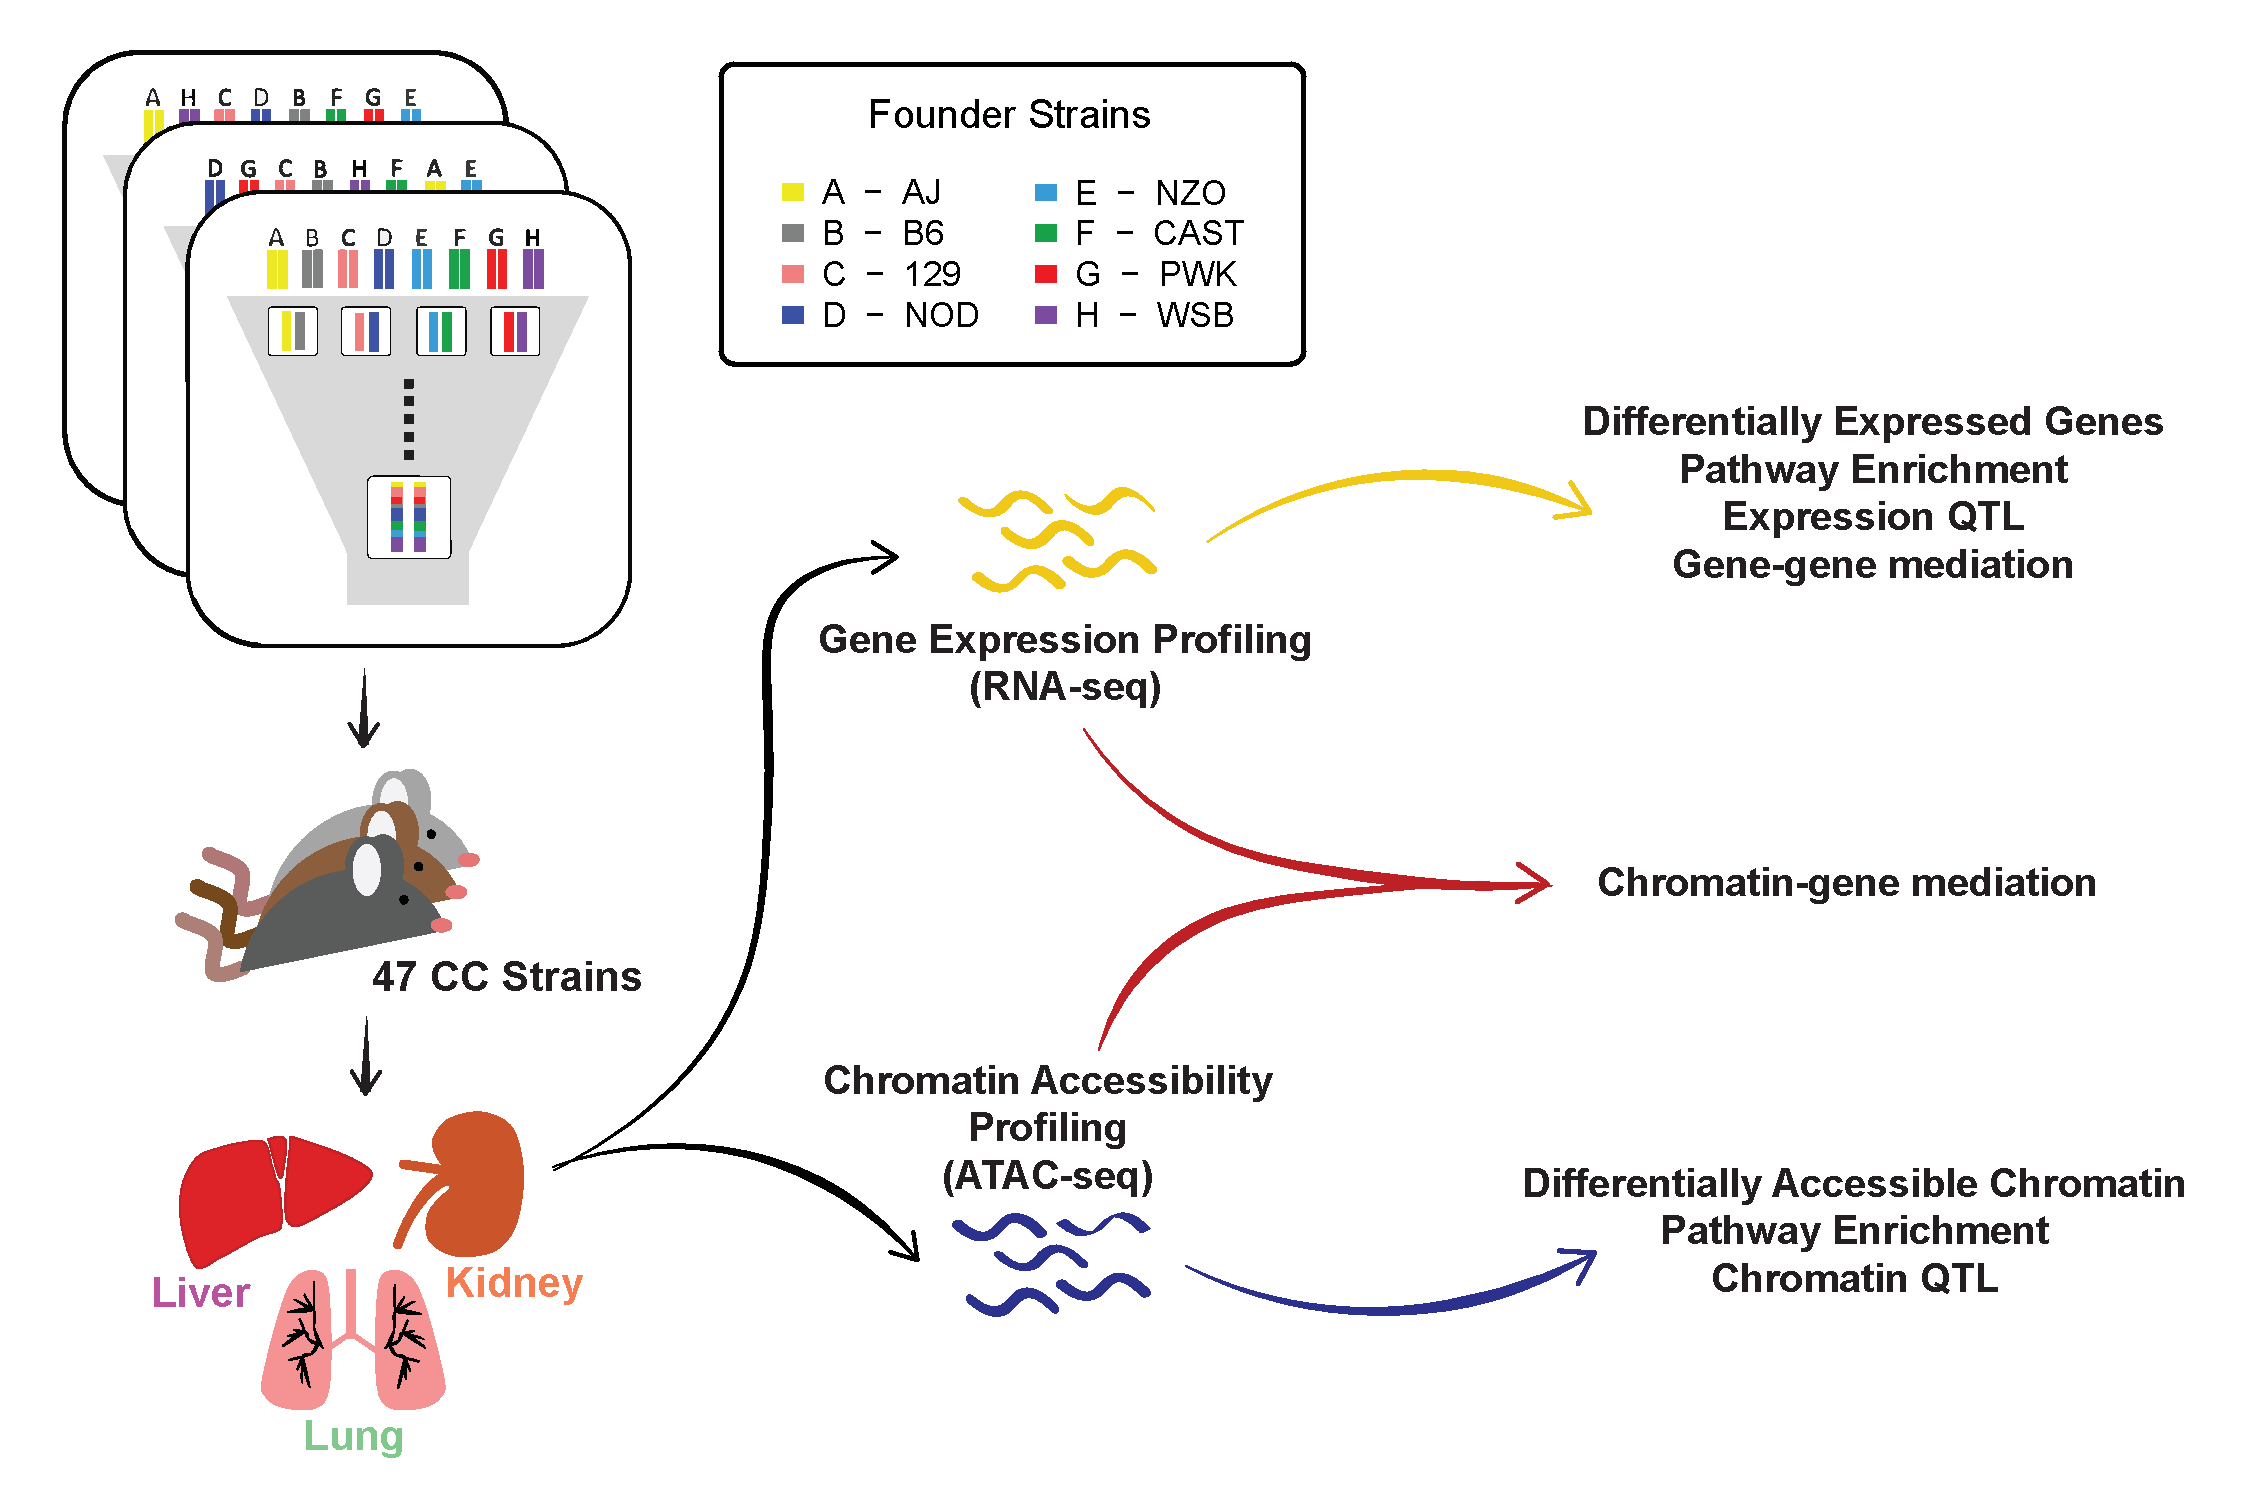
\includegraphics[width=0.8\linewidth, clip, trim={0in 0.1in 0in 0.2in}]{figs/overview_diagram_simplified.pdf}
\caption{\textbf{Diagram of the experiment and analyses.} RNA-seq and ATAC-seq were collected from liver, lung, and kidney tissues of males from 47 CC strains. Each CC strain was derived from an inbreeding funnel, and thus represents a recombinant inbred mosaic of the initial eight founder haplotypes. Differential analyses with pathway enrichment analyses were performed to identify biological pathways enriched in differentially expressed genes and accessible chromatin regions. QTL and mediation analyses were performed to identify regions that causally regulate gene expression and chromatin accessibility.
\label{fig:overview}}
\end{figure*}

\subsection{Animals}

Adult male mice (8-12 weeks old) from 47 CC strains were acquired from the University of North Carolina Systems Genetics Core (listed in \textbf{Appendix A}) and maintained on an NTP 2000 wafer diet (Zeigler Brothers, Inc., Gardners, PA) and water \textit{ad libitum}. The housing room was maintained on a 12-h light-dark cycle. Our experimental design sought to maximize the number of strains relative to within-strain replications based on the power analysis for QTL mapping in mouse populations \citep{Kaeppler1997}; therefore, one mouse was used per strain. Mice were euthanized and lungs, liver and kidney tissues were collected, flash frozen in liquid nitrogen, and stored at -80\degree C. These studies were approved by the Institutional Animal Care and Use Committees at Texas A\&M University and the University of North Carolina. The experiment and subsequent analyses performed for this study are diagrammed in \textbf{Figure \ref{fig:overview}}.

\subsection{mRNA sequencing and processing}

Total RNA was isolated from flash-frozen tissue samples using a Qiagen miRNeasy Kit (Valencia, CA) according to the manufacturer’s protocol. RNA purity and integrity were evaluated using a Thermo Scientific Nanodrop 2000 (Waltham, MA) and an Agilent 2100 Bioanalyzer (Santa Clara, CA), respectively. A minimum RNA integrity value of 7.0 was required for RNA samples to be used for library preparation and sequencing. Libraries for samples with a sufficient RNA integrity value were prepared using the Illumina TruSeq Total RNA Sample Prep Kit (Illumina, Inc., San Diego, USA) with ribosomal depletion. Single-end (50 bp) sequencing was performed (Illumina HiSeq 2500).

Sequencing reads were filtered (sequence quality score $\ge$ 20 for $\ge$ 90\% of bases) and adapter contamination was removed (TagDust). Reads were mapped to strain-specific pseudo-genomes (Build37, \url{http://csbio.unc.edu/CCstatus/index.py?run=Pseudo}) and psuedo-transcriptomes (C57BL/6J RefSeq annotations mapped to pseudo-genomes) using RSEM with STAR (v2.5.3a). Uniquely aligned reads  were used to quantify expression as transcripts per million (TPM) values.

\subsection{ATAC-seq processing}

Flash frozen tissue samples were pulverized in liquid nitrogen using the BioPulverizer (Biospec) to break open cells and allow even exposure of intact chromatin to Tn5 transposase \citep{Buenrostro2015}. Pulverized material was thawed in glycerol containing nuclear isolation buffer to stabilize nuclear structure and then filtered through Miracloth (Calbiochem) to remove large tissue debris. Nuclei were washed and directly used for treatment with Tn5 transposase. Paired-end (50 bp) sequencing was performed (Illumina HiSeq 2500).

Reads were similarly filtered as with RNA-seq. Reads were aligned to the appropriate pseudo-genome using GSNAP (parameter set: -k 15, -m 1, -i 5, –sampling=1, –trim-mismatch-score=0, –genome-unk-mismatch=1, –query-unk-mismatch=1). Uniquely mapped reads were converted to mm9 mouse reference genome coordinates using the associated MOD files (UNC) to allow comparison across strains. Reads overlapping regions in the mm9 blacklist (UCSC Genome Browser) were removed. Exact sites of Tn5 transposase insertion were determined as the start position +5 bp for positive strand reads, and the end position -5 bp for negative strand reads \citep{Buenrostro2013}. Peaks were called using F-seq with default parameters. A union set of the top 50,000 peaks (ranked by F-seq score) from each sample was derived. Peaks were divided into overlapping 300 bp windows as previously described \citep{Shibata2012}. Per sample read coverage of each window was calculated using coverageBed from BedTools \citep{Quinlan2010}.

\subsection{Sequence trait filtering for QTL analysis}

Trimmed mean of M-values (TMM) normalization [edgeR, \citep{edgeR}] was applied to TPM values from read counts of genes and chromatin windows, respectively. Genes with TMM-normalized TPM values $\leq$ 1 and chromatin windows with normalized counts $\leq$ 5 for $\geq$ 50\% of samples were excluded. For each gene and chromatin window, we applied $K$-means clustering with $K=2$ to identify outcomes containing outlier observations that could cause spurious, outlier-driven QTL calls. Any gene or chromatin window where the smaller $K$-means cluster had a cardinality of 1 was removed.

\subsection{CC strain genotypes and inferred haplotype mosaics}

CC genomes are mosaics of the founder strain haplotypes and were previously reconstructed by the UNC Systems Genetics Core (\url{http://csbio.unc.edu/CCstatus/index.py?run=FounderProbs}) with the Hidden Markov Model of \cite{Fu2012} on genotype calls [MegaMUGA array \citep{Morgan2016muga}] from multiple animals per strain. To reduce the number of statistical tests, adjacent genomic regions were merged through averaging if the founder mosaics for all mice were similar, defined as L2 distance $\leq$ 10\% of the maximum L2 distance ($\sqrt{2}$ for a probability vector), which reduced the number of tested loci from 77,592 to 14,191.

\subsection{Differential expression and accessibility analyses}

Read counts for each sample were converted to counts per million (CPM) and normalized using TMM normalization (\textit{edgeR}). Windows with > 70 \% of samples with CPM $\leq$ 1 were removed. Differentially expressed genes and accessible chromatin windows were determined using \textit{limma} \citep{limma} using a linear model with TMM-normalized CPM value as the response and fixed effect covariates of strain, batch and tissue (lung, liver, or kidney). 
To account for mean-variance relationships in gene expression and chromatin accessibility data, precision weights were calculated using the \textit{limma} function \textit{voom} and incorporated into the linear modeling procedure. The $p$-values were adjusted using a false discovery rate (FDR) procedure \citep{Benjamini1995}, and differentially expressed genes and accessible chromatin windows were called based on the q-value $\le$ 0.01 and log$_{2}$ fold-change $\geq$ 1. Adjacent significantly differential chromatin windows in the same direction were merged with a $p$-value computed using Simes' method \citep{Sarkar1997}, and chromatin regions were re-evaluated for significance using the Simes $p$-values.

\subsection{Gene set association analysis}

Biological pathways enriched with differentially expressed genes or accessible chromatin were identified with GSAASeqSP \citep{Xiong2014} with Reactome Pathway Database annotations (July 24, 2015 release). A list of assayed genes were input to GSAASeqSP along with a weight for each gene $g$, calculated as:
\begin{equation}
\text{weight}_{g} = \text{sign}(\text{fc}_{g}) \times (1-q_{g}),
\label{eq:gene_weighting}
\end{equation}
where $\text{sign}(\text{fc}_{g})$ is the sign of the expression fold change, and $q_{g}$ is the FDR-adjusted $p$-value. Pathways with gene sets of cardinality < 15 or > 500 were excluded. For chromatin accessibility, each region was mapped to a gene using GREAT v3.0.0 (\textit{basal plus extension} mode, \textit{5 kb upstream}, \textit{1 kb downstream}, and no distal extension). \GKinline{Each gene was then paired with the chromatin region with the smallest FDR-adjusted $p$-value. Gene weights were calculated as with gene expression, but with $\text{sign}(\text{fc}_{g})$ representing the sign of chromatin accessibility fold-change and $q_{g}$ the FDR-adjusted $p$-value of the chromatin region paired wigh gene $g$.}

%\begin{table*}[h]
%\renewcommand{\familydefault}{\sfdefault}\normalfont
%\begin{tableminipage}{\textwidth}
%\captionsetup{width=\textwidth}
%\centering
%\caption{\bf QTL mapping procedures \WVinline{Not useful as is, should probably delete.}
%\label{tab:qtl_procedures}}
%\end{tableminipage}
%\begin{tableminipage}{\textwidth}
%\begin{tabularx}{\textwidth}{l | cccc}
%\hline 
%Procedure & QTL type & FWER control & FDR control & QTL per trait \\
%\hline
%Method 1 & local \& distal & genome-wide & yes & $\ge$ 1 \\
%Method 2 & local \& intra-chromosomal distal & chromosome-wide & yes & 1 \\
%Method 3 & local & genome \& chromosome-wide & no & 1 \\
%\hline
%\end{tabularx}
%\end{tableminipage}
%\end{table*}

\subsection{QTL model}

QTL analysis was performed for both gene expression and chromatin accessibility using regression on inferred haplotypes \citep{Mott2000}, a variant of Haley-Knott regression \citep{Haley1992,Martinez1992} commonly used for mapping in the CC \citep{Valdar2006c,Aylor2011,Gralinski2015,Kelada2016,Donoghue2017,Keele2019} and other multiparent populations (MPPs) [\eg, \citet{King2012} in \textit{Drosophila}].

For a given trait, at each of the 14,191 loci in the genome, we fitted the linear model,
\begin{equation}
  y_i = \mu + \text{batch}_i + \text{QTL}_i + \varepsilon_i\, \label{eq:alternative_model}
\end{equation}
where $y_{i}$ is the trait, either levels of gene expression or chromatin accessibility for individual $i$, $\mu$ is the intercept, $\text{batch}_i$ is a categorical fixed effect covariate \GKinline{representing five sequencing batches for both gene expression and chromatin accessibility}, $\varepsilon_i\sim\text{N}(0,\sigma^2)$ models the residual error, and $\text{QTL}_{i}$ models the genetic effect at the locus. Specifically, the QTL term models the (additive) effects of alternate haplotype states and is defined as $\text{QTL}_{i}=\bbeta\T\bx_i$, where $\bx_i=(x_{i,\text{AJ}},\dots,x_{i,\text{WSB}})\T$ is a vector of dosages, \ie, expected counts (0-2) from the haplotype reconstruction, for the eight founder haplotypes and $\bbeta=(\beta_\text{AJ},\dots,\beta_\text{WSB})\T$ is a corresponding vector of fixed effects. (Note that in fitting this term as a fixed effects model, the linear dependency among the dosages in $\bx_i$ results in at least one founder haplotype effect being omitted to achieve identifiability; see later). Prior to model fitting, to avoid sensitivity to non-normality and strong outliers, the response $\{y_i\}^n_{i=1}$ was subject to a rank inverse normal transformation (RINT).
The fit of \autoref{eq:alternative_model} was compared with the fit of the same model omitting the QTL term (the null model) by an F-test, leading to a nominal $p$-value, reported as the $\text{logP}=-\log_{10}(\text{$p$-value})$. A QTL was detected if this logP surpassed a set significance threshold, described below. %in \textbf{Appendix A}. 

%In this form of QTL mapping, which is a type of linkage disequilibrium (LD) mapping or haplotype association, the genotypes of the individuals are not used for association directly; rather, they are used to obtain a probabilistic reconstruction of the underlying mosaic of founder haplotypes, and association is performed on that underlying haplotype mosaic instead. This allows a wider range of trait variants to be detected since the haplotypes implicitly model not only multi-allelic variants but also all local epistatic interactions [\eg, arguments in \citet{Zhang2014}]; it also clearly reveals the LD pattern and therefore the realistic limits of mapping resolution.

%A single locus approach to QTL mapping was used for both gene expression and chromatin accessibility. The CC mice have well-characterized founder haplotypes, allowing the association analysis to be haplotype-based, also referred to as interval mapping or linkage analysis \citep{Lander1989}. Assessing association between haplotype descent and phenotype has advantages to variant association, such as implicitly modeling multiple local variants simultaneously and more closely reflecting the linkage disequilibrium (LD) decay. Because haplotype state is not directly observed but rather probabilistically inferred (\eg \citealt{Lander1987,Mott2000,Liu2010,Fu2012,Gatti2014,Zheng2015}), formal interval mapping requires an computationally inefficient Expectation-Maximization (EM) algorithm \citep{Dempster1977}. A computationally efficient regression approximation \citep{Haley1992,Martinez1992} is commonly used instead for multiparental populations (MPP) (\eg \citealt{Valdar2006a,Valdar2009,Svenson2012,Baud2013,Baud2014}), including the CC (\eg \citealt{Aylor2011,Kelada2016,Mosedale2017,Donoghue2017}). This efficiency is particularly important in the context of a study of genome-wide molecular phenotypes.

\subsection{\GKinline{Significance thresholds}}

\GKinline{Thresholds were determined based on permutations specific to each trait. The appropriateness of permutation-derived thresholds \citep{Doerge1996} is dependent on the CC having balanced founder haplotype contributions. This assumption was supported by simulations of the funnel breeding design \citep{Valdar2006c}, though recently \cite{Keele2019} performed simulations of the observed CC strain genomes and found low levels of population structure for highly polygenic genetic architectures. As such, we use permutations given that molecular traits often have strong effect QTL that are detectable in the presence of subtle population structure.}

\GKinline{1,000 permutations of the sample index were recorded, and then genome scans performed for each trait, using the same permutations. Given a trait, the maximum logP, from either the entire genome or the local chromosome, for each permutation was collected, and used to fit a null extreme value distribution (EVD) \citep{Dudbridge2004}. Genome-wide and local chromosome-wide thresholds were calculated as the 95\textsuperscript{th} upper quantile of the respective EVDs.}

\subsection{\GKinline{QTL mapping procedures}}
%\WVinline{Redo this section --- needs more, see note.}} \WV{Three mapping procedures were used to detect QTL, each with unique features:}{This section must start with a rationale (why does it make sense to have three methods?), prefably a more precise version of the one currently in the Discussion. The three methods described here need more description. At present they cannot be understood without the Appendix. Also, I don't find Table 1 useful or understandable. Delete Table 1 and just try to make this section clear.}
%\begin{enumerate}[label = \method{{\arabic*:}}]
%\setlength{\itemindent}{3em}
\GKinline{We used three related procedures for calling eQTL and cQTL at varying levels of statistical significance while taking into account local/distal status of putative QTL.}

\subsubsection{\GKinline{Local analysis - Analysis L.}} 
\GKinline{We first detected local-QTL, leveraging the prior belief in local genetic regulation, here on referred to as Analysis L. Genome-wide scans were performed for all traits, and a QTL was detected if the peak association (measured as logP) within 10Mb of the gene transcription start site (TSS) or chromatin region midpoint surpasses the significance threshold. QTL were called with respect to both genome-wide and local chromosome-wide thresholds.}

\subsubsection{\GKinline{Local chromosome analysis - Analysis LC.}} 
\GKinline{We next expand the scope of potential detected QTL to include any locus on the chromosome that harbors the trait, \ie the local chromosome, here after referred to as Analysis LC. These results are drawn from the same genome scans as Analysis L; however, instead of considering only the local window around the trait's genomic coordinate, the peak logP on the local chromosome is adjusted to control the family-wise error rate (FWER) based on the local chromosome EVD, denoted as permP. Additionally, we adjust the permP to control the FDR (at both 0.1 and 0.2), accounting for multiple testing across the traits. See \textbf{Appendix B} for further discussion on false positive control.}

\GKinline{In comparison to Analysis L, this procedure is more stringent on local-QTL because of the additional FDR adjustment. Alternatively, it is highly lenient in detecting distal-QTL located on the local chromosome. Notably, Analysis LC would not detect QTL within the local window if a stronger association is observed outside the window, though Analysis L would.}

\subsubsection{\GKinline{Genome-wide analysis - Analysis G.}} 
\GKinline{Our final approach for detecting QTL, referred to as Analysis G, is the most statistically stringent, only identifying genome-wide significant QTL that pass FDR control. Analysis G also uses the same genome scans as Analyses L and LC, but incorporates additional scans conditioned on detected QTL to potentially identify multiple QTL per trait in unbiased fashion for FDR. Notably, the local status of the QTL does not factor into Analysis G. See \textbf{Appendix D} for details on the conditional genome scan procedure.}

\GKinline{Analyses L, LC, and G potentially detect many of the same QTL, specifically strong local-QTL. Collectively, they allow for efficient detection of QTL with varying degrees of statistical support while strongly leveraging local status.}

%\begin{description}
%	\item[Method 1:] Multi-stage conditional regression with genome-wide family-wide error rate (FWER) and FDR control (Method 1). This procedure is the most statistically stringent, can identify both local and distal-QTL, and potentially multiple QTL per trait in an unbiased FDR control.
%    \item[Method 2:] Single-stage regression with chromosome-wide FWER and FDR control (Method 2). This procedure is oriented towards identification of local-QTL by using the much more lenient chromosome-wide FWER adjustment. Putative distal-QTL that are located on the same chromosome as the target but are not proximal to the trait's genomic coordinate are also leniently detected, referred to here as intra-chromosomal distal-QTL.
%    \item[Method 3:] Single-stage regression with genome-wide and chromosome-wide FWER control (Method 3). This procedure only detects local-QTL, leveraging strong biological precedent for local genetic regulation to reduce the significance threshold. FWER adjustment, either at genome or chromosome-wide levels, is performed for the maximum logP in the local window (defined here as 10Mb upstream or downstream of target's coordinate), without FDR control.
%\end{description}

%See \textbf{Appendix C} for greater detail on the mapping procedures.

\subsubsection{QTL effect size.}

%\WV{}{I removed the shrinkage estimation of QTL effect size. I can't see that it adds anything and, anyway, estimation of effect size based on a variance component controlling 8 variables is pretty unstable and probably not something we want to advocate.}
The effect size of a detected QTL was defined as the $R^2$ attributable to the QTL term; specifically, as $1-\text{RSS}_\text{QTL} / \text{RSS}_0$, where $\text{RSS} = \sum_{i = 1}^{n}(y_{i} - \widehat{y_{i}})^{2}$ is the residual sum of squares, \ie, the sum of squares around predicted value $\widehat{y_i}$, and $\text{RSS}_{\text{QTL}}$ and $\text{RSS}_0$ denote the RSS calculated for the QTL and null models respectively. \GKinline{We also estimated a conservative QTL effect size estimate with a QTL random effects model, which is compared with the $R^{2}$ estimate in \textbf{Figures \ref{fig:qtl_effect_size_fixefvsranef}}}

\subsubsection{QTL effects: estimating BLUPs for effects of founder haplotypes.} 

%\WV{}{These are often referred to in the MS as ``founder allele'' effects. However, the term allele is confusing here since we don't know the allelic series of a particular QTL and some founder haplotypes will in fact share the same allele. So ``founder allele'' should be substituted with ``founder haplotype'' or simply ``haplotype''}
%The effects of each founder haplotype at a detected QTL were estimated using a model similar to that used for mapping but with an dadditional shrinkage component to ensure estimates were stable. 
The fixed effects QTL model used for mapping, though powerful for detecting associations, is suboptimal for providing stable estimates of the haplotype effects vector, $\bbeta$. This is because, among other things, 1) the matrix of haplotype dosages that forms the design matrix of $\{\text{QTL}_i\}^n_{i=1}$ in Eq \ref{eq:alternative_model}, is multicollinear, which leads to instability, and 2) because the number of observations for some haplotypes will often be few, leading to high estimator variance \citep{Zhang2014}. More stable estimates were therefore obtained using shrinkage. At detected QTL, the model was refit with $\bbeta$ modeled as a random effect, $\bbeta \sim \text{N}(\bzero, \bI\tausq)$ [as in \citet{Wei2016}], to give an 8-vector of best linear unbiased estimates [BLUPs, \citet{Robinson1991}], $\blup=(\widetilde{\beta}_\text{AJ},\dots,\widetilde{\beta}_\text{WSB})\T$. These BLUPs, after being centered and scaled, were then used for further comparison of QTL across tissues. 

%The founder allele effects at a QTL, as fit in the mapping model (Eq \ref{eq:alternative_model}), can help distinguish which genetic variants drive an observed QTL. However, these effects, when pulled directly from the mapping procedures, are comprised of a vector with one fixed effect regression coefficient per founder strain and can be unstable when there are few observations per founder strain contribution at a locus, resulting in artificially extreme effects \citep{Zhang2014}. To conservatively constrain the effect estimates, the model in Eq \ref{eq:alternative_model} was re-fit at the detected QTL, but with the QTL effect as a random effect vector with corresponding variance component \citep{Wei2016}, such that $\text{QTL}_{i} = \bx_{i}\bbeta$ with $\bbeta \sim \text{N}(\bzero, \bI\tausq)$. $\bx_{i}$ is the founder haplotype dosage vector for individual $i$ at the QTL, $\bbeta$ is the QTL effect vector, and $\tausq$ is the variance component corresponding to the QTL effect vector. The best linear unbiased predictors of the allele effects [$\widehat{\bbeta}_{\text{BLUP}}$] \citep{Robinson1991} were calculated, centered and scaled, and used for further comparison of QTL across tissues. 

\subsubsection{Comparing QTL effects across tissues.}

To summarize patterns of the genetic regulation of gene expression and chromatin accessibility across tissues, we calculated correlations between the founder haplotype effects of QTL that map to approximately the same region of the genome for the same traits but in different tissues. For pairs of local-QTL, it was required that both be detected within the 20Mb window around the gene TSS or the chromatin window midpoint. For pairs of distal-QTL, the QTL positions had to be within 10Mb of each other. All detected QTL were considered, including QTL from Analyses G and LC controlled at an FDR of 0.2, allowing for consistent signal across tissues to provide further evidence for putative QTL with marginal significance within a single tissue.

Correlations were performed as follows. For a pair of matched QTL $j$ and $k$ from different tissues, we calculated the Pearson correlation coefficient of their QTL effect BLUPs, $r_{jk} = \text{cor}(\blup_j, \blup_k)$. Since each $\blup$ is an 8-element vector, the corresponding $r$ are distributed such that $r\sqrt{6}(1 - r^{2})^{-1} \sim t_{6}$ according to the null model of independent variables. Testing alternative models of $r_{jk} > 0$ and $r_{jk} < 0$ produced two $p$-values per pair of QTL. These were then subject to FDR control \citep{Benjamini1995} to give two q-values, $q_{ij}^{\{r > 0\}}$ and $q_{ij}^{\{r < 0\}}$, and these were used to classify pairs of QTL as being significantly correlated or anti-correlated, respectively. 

\subsubsection{Variant association.}

Variant association was performed within the genomic regions surrounding overlapping QTL in order to detect similarities and differences in patterns of association between tissues, \GKinline{potentially distinguishing distinct tissue-specific QTL from those observed in multiple tissues}. Variant genotypes from Build38 were obtained using the ISVdb \citep{Oreper2017} for the CC strains, which were converted to Build37 coordinates with the liftOver tool \citep{Lawrence2009}. Variants were filtered out if their minor allele frequencies $\le 0.1$ or they were not genotyped in one of the CC founder strains to avoid false signals.

\begin{figure}[htbp]
\renewcommand{\familydefault}{\sfdefault}\normalfont
\centering
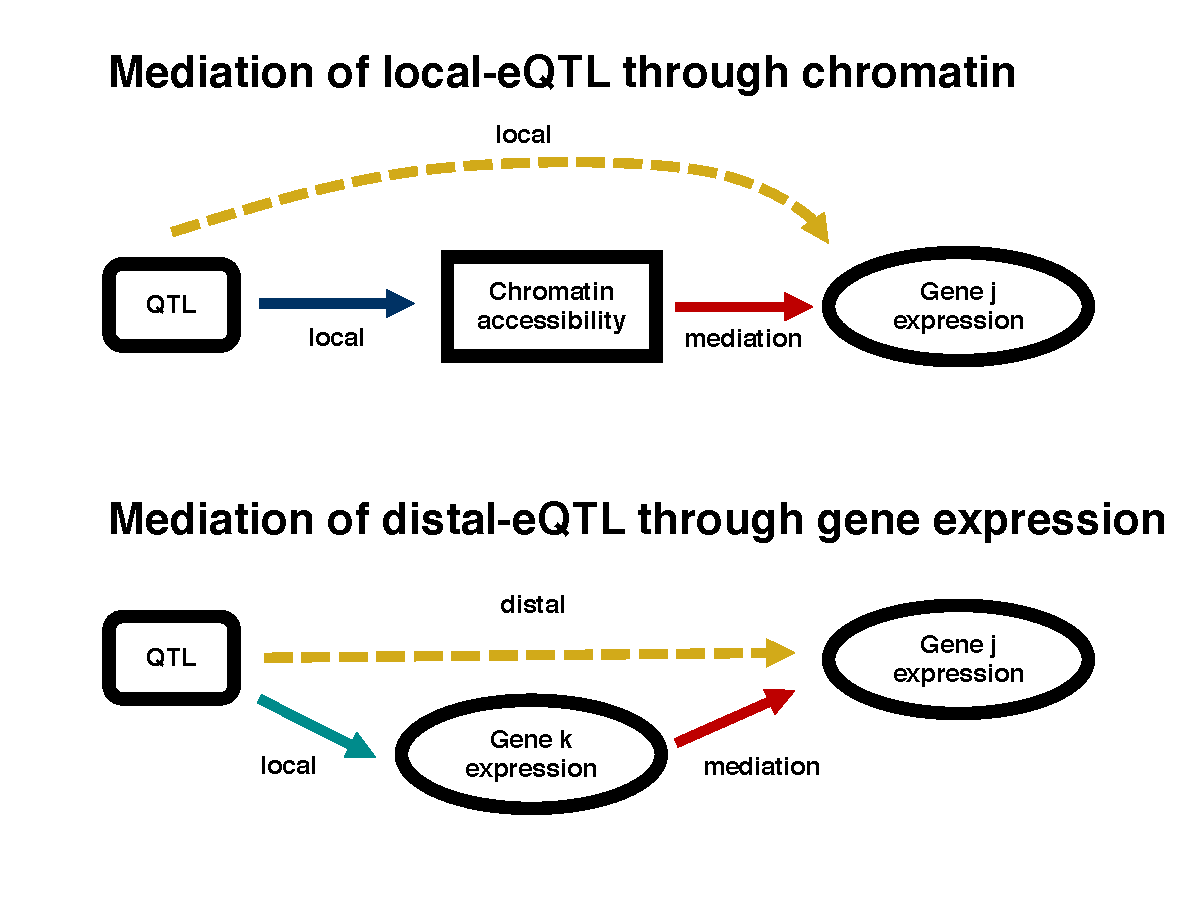
\includegraphics[width=\linewidth, clip, trim={0in 0.5in 0in 0in}]{figs/mediation_graph.pdf}
\caption{\textbf{Simple mediation models for the genetic regulation of gene expression.} Mediation of the local-eQTL through chromatin accessibility in the region of the gene (A) is consistent with genetic variation influencing the accessibility of gene j to the transcriptional machinery. Mediation of distal-eQTL through the transcription of genes local to the QTL (B) could be explained by transcription factor activity. 
\label{fig:graph}}
\end{figure}

\subsection{Mediation analysis}

Mediation analyses have recently been used with genomic data, including in humans (\eg \citealt{Battle2014}). We use a similar approach to \cite{Chick2016} and \cite{Keller2018} to assess statistically significant mediation of eQTL effects on gene expression.

Detection of mediation is dependent on a number of assumptions about the underlying variables, their relationships, and the directionality of those relationships, many of which cannot be satisfied in a system as complex as chromatin accessibility and transcriptional regulation in whole living organisms. However, signals in the data that are consistent with the mediation model could identify putative causal factors that regulate gene expression. The mediation models tested here are represented in \textbf{Figure \ref{fig:graph}}.

The mediation relationships are evaluated in a genome-wide scan, allowing for the detection of statistically significant candidate mediators. Similar to the QTL mapping genome scan described in Eq \ref{eq:alternative_model}, the mediation scan involves a comparison of an alternative and a null model at loci across the genome. The alternative model is
\begin{equation}
y^{\text{G}_{j}}_{i} = \mu + \text{eQTL}_{i}^{\text{G}_{j}} + m_{ik} + \text{batch}_{i} + \varepsilon_{i},
\label{eq:mediation_alt}
\end{equation}
which is compared with the null model:
\begin{equation}
y^{\text{G}_{j}}_{i} = \mu + m_{ik} \nonumber + \text{batch}_{i} + \varepsilon_{i}
\label{eq:mediation_null}
\end{equation}
where $y^{\text{G}_{j}}_{i}$ is the expression levels for individual $i$ of gene $j$ with an eQTL, $\mu$ is the intercept term, $\text{eQTL}_{i}^{\text{G}_{j}}$ is the eQTL effect on gene $j$, $m_{ik}$ is the effect of the $k$\textsuperscript{th} mediator, either chromatin accessibility or gene expression depending on the mediation model being evaluated, $\text{batch}_{i}$ is the effect of the sequencing center, and $\varepsilon_{i}$ is random noise. Conditioned loci can be included for certain eQTL, as in Eq \ref{eq:conditional_model}, but not included here for clarity. Whereas with the QTL genome scan, the locus effect was changed at each position, for the mediation scan, it is fixed at the eQTL locus, and the mediator is changed.

Because the eQTL is always included in the alternative model but not the null model, the logP of the mediation scan should fluctuate around the observed eQTL logP. At mediators that possess some or all of the information present in the eQTL, the logP will drop. Significant logP drops represent candidate mediators. Significance thresholds to control FWER were determined by performing mediation scans on 1,000 permutations of the mediator variable. See \textbf{Appendix D} for further discussion and greater detail on the mediation analysis, including permutation approach to significance thresholds and the formal criterion for mediation detection.

\subsection{Software and Data Availability}

All statistical analyses were conducted with the R statistical programming language \citep{RSoftware2019}. The R package miQTL was used for all the mapping and mediations analyses, and is available on GitHub at \url{https://github.com/gkeele/miqtl}. A static version of miQTL is also provided in the \textbf{Supplement} (File S2).

The data, results files, and scripts to generate the results are provided in the \textbf{Supplement}, described in File S1. All files are available at figshare. File S3 contains the founder haplotype mosaics used for this study in a format that works with miQTL. Files S4 - S9 are the processed gene expression and chromatin accessibility data for liver, lung, and kidney used in the differential and QTL analyses. Files S10 - S12 are results tables of differentially expressed genes for (liver/lung), (liver/kidney), and (lung/kidney); and Files S13 - S15 are results tables for differentially accessible regions. Files S16 - S18 are the local-eQTL results tables for liver, lung, and kidney, respectively; Files S19 - S21 are distal-eQTL results tables; Files S22 - S24 are local-cQTL results tables; and Files S25 - S27 are distal-cQTL results tables. Files S28 - S30 are results tables of local-eQTL with chromatin mediators. File S31 is the supplemental tables and figures.

%%%%%%%%%% Results
\section{Results}

%\WV{}{Please use headlines where possible. Note: a headline is what you found, not what you did or a general subject area.}

\subsection{Differential gene expression and chromatin accessibility} %\WVinline{[Convert to (or add a) headline]}}

\subsubsection{Gene expression and chromatin accessibility cluster by tissue.}
Gene expression and chromatin accessibility, using RNA-seq and ATAC-seq respectively, were measured in lung, liver, and kidney tissues in one male mouse from each of 47 CC strains. As the function of each tissue is quite distinct, we expected that these data would reflect tissue-specific differences. Principal components analysis (PCA) of each of the gene expression and chromatin accessibility profiles shows that the samples clearly cluster by tissue (\textbf{Figure \ref{fig:pca_plots}}). 

\subsubsection{Differentially expressed genes strongly correspond with accessible chromatin regions.} We performed pairwise differential expression (DE) and differentially accessible region (DAR) analysis between the three tissues (\textbf{Table \ref{tab:diff_gene}}), and found between 3,564 - 5,709 DE genes, and 28,048 - 40,797 DARs (FWER < 0.1). For both expression and chromatin accessibility, liver and kidney tissues were the most similar, and lung and liver the most distinct, which was also reflected in the PCA plots. Pathway analyses showed many between-tissue differences related to metabolic and immune-related pathways (FWER < 0.1), reflecting the distinct demands of each tissue. Energy metabolism pathways were more active in liver and kidney and immune-related pathways were more pronounced in lung. We compared the concordance between DE genes and DARs genome-wide and observed that most DE gene promoters do not show significant differences in chromatin accessibility (\textbf{Figure \ref{fig:diff_concordance}}). In cases where there were significant variability in accessibility at the promoter of a DE gene, though, the vast majority agree in direction (\ie, higher expression with greater accessibility).

\subsection{Tissue-specific expression QTL}

To evaluate the impact of genetic variation on gene expression, we performed eQTL mapping using three \GKinline{scopes of analysis: the local region of a gene (defined as within 10Mb of the gene TSS; Analysis L), the local chromosome (Analysis LC), and genome-wide (Analysis G). Additionally, we classify distal-eQTL located on the local chromosome as intra-chromosomal, and otherwise inter-chromosomal.}
% to detect eQTL were used (\textbf{Table \ref{tab:qtl_procedures}}), summarized here and described more completely in \textbf{Appendix B}. 
%Analysis L was also a single-step analysis and employed an even more lenient significance criteria based on the genome-wide and chromosome-wide adjusted FWER $p$-value. 
%Analysis LC was less stringent, requiring FDR-controlled significance at a chromosome-wide level and only using results from the first stage of the multi-stage analysis, which we refer to as a single-step analysis. 
%Analysis G was the most stringent and involved a multi-stage conditional regression procedure paired with an FDR control that allowed for the detection of potentially multiple eQTL per gene and required significance at a genome-wide level.
%We classified local-eQTL as being within 10Mb of the gene TSS, and distal-eQTL as being greater than 10Mb from the TSS on the same chromosome (intra-chromosomal) or on a different chromosome (inter-chromosomal). 
%For Analysis LC, only local-eQTL and intra-chromosomal distal-eQTL were detected due to our use of chromosome-wide significance criteria. 
%For Analysis L, the least stringent method, we only detected local-eQTL.

After filtering out lowly expressed genes, the number of genes considered in eQTL mapping was 8401 for liver, 11357 for lung, and 10092 for kidney; a breakdown of the genes analyzed per tissue for QTL analysis is provided in \textbf{Figure \ref{fig:upset_genes_chromatin}A} using an UpSet plot \citep{Conway2017}. 
%Positions of local-eQTL detected for each tissue using any of the three methods (Analysis G, genome-wide q-value < 0.1; Analysis LC, chromosome-wide q-value < 0.1; Analysis L, genome-wide and chromosome-wide FWER $p$-value < 0.05)  are shown in \textbf{Figure \ref{fig:grid_plot}A} (light colored dots), as well as summarized in \textbf{Table \ref{tab:eqtl_mapping}}. 
Positions of eQTL detected for each tissue are shown in \textbf{Figure \ref{fig:grid_plot}A}, with local-eQTL (light colored dots) detected through Analysis L and distal-eQTL (dark colored dots) detected through Analysis G, as well as summarized in \textbf{Table \ref{tab:eqtl_mapping}}. 
We also identified eQTL with Analyses LC and G using a more relaxed significance threshold (q-value < 0.2; \textbf{Figure \ref{fig:grid_fdr_plot}A} and \textbf{Table \ref{tab:eqtl_mapping_lenient}}). Increasing the FDR threshold from 0.1 to 0.2 increases the number of distal-eQTL detected to a greater extent than local-eQTL. Using Analysis L and requiring genome-wide significance, the percentage of tested genes with local-eQTL were 6.3\% for lung, 8.4\% for liver, and 9.5\% for kidney (\textbf{Table \ref{tab:eqtl_mapping}}). These percentages increase to 16.6\%, 19.8\%, and 20.8\% respectively when criteria were less stringent with only chromosome-wide significance \GKinline{with Analysis L}. Most genes with local-eQTL were observed in only one tissue (\textbf{Figure \ref{fig:upset_eqtl_cqtl}A}).

\begin{figure*}[h]
\renewcommand{\familydefault}{\sfdefault}\normalfont
\centering
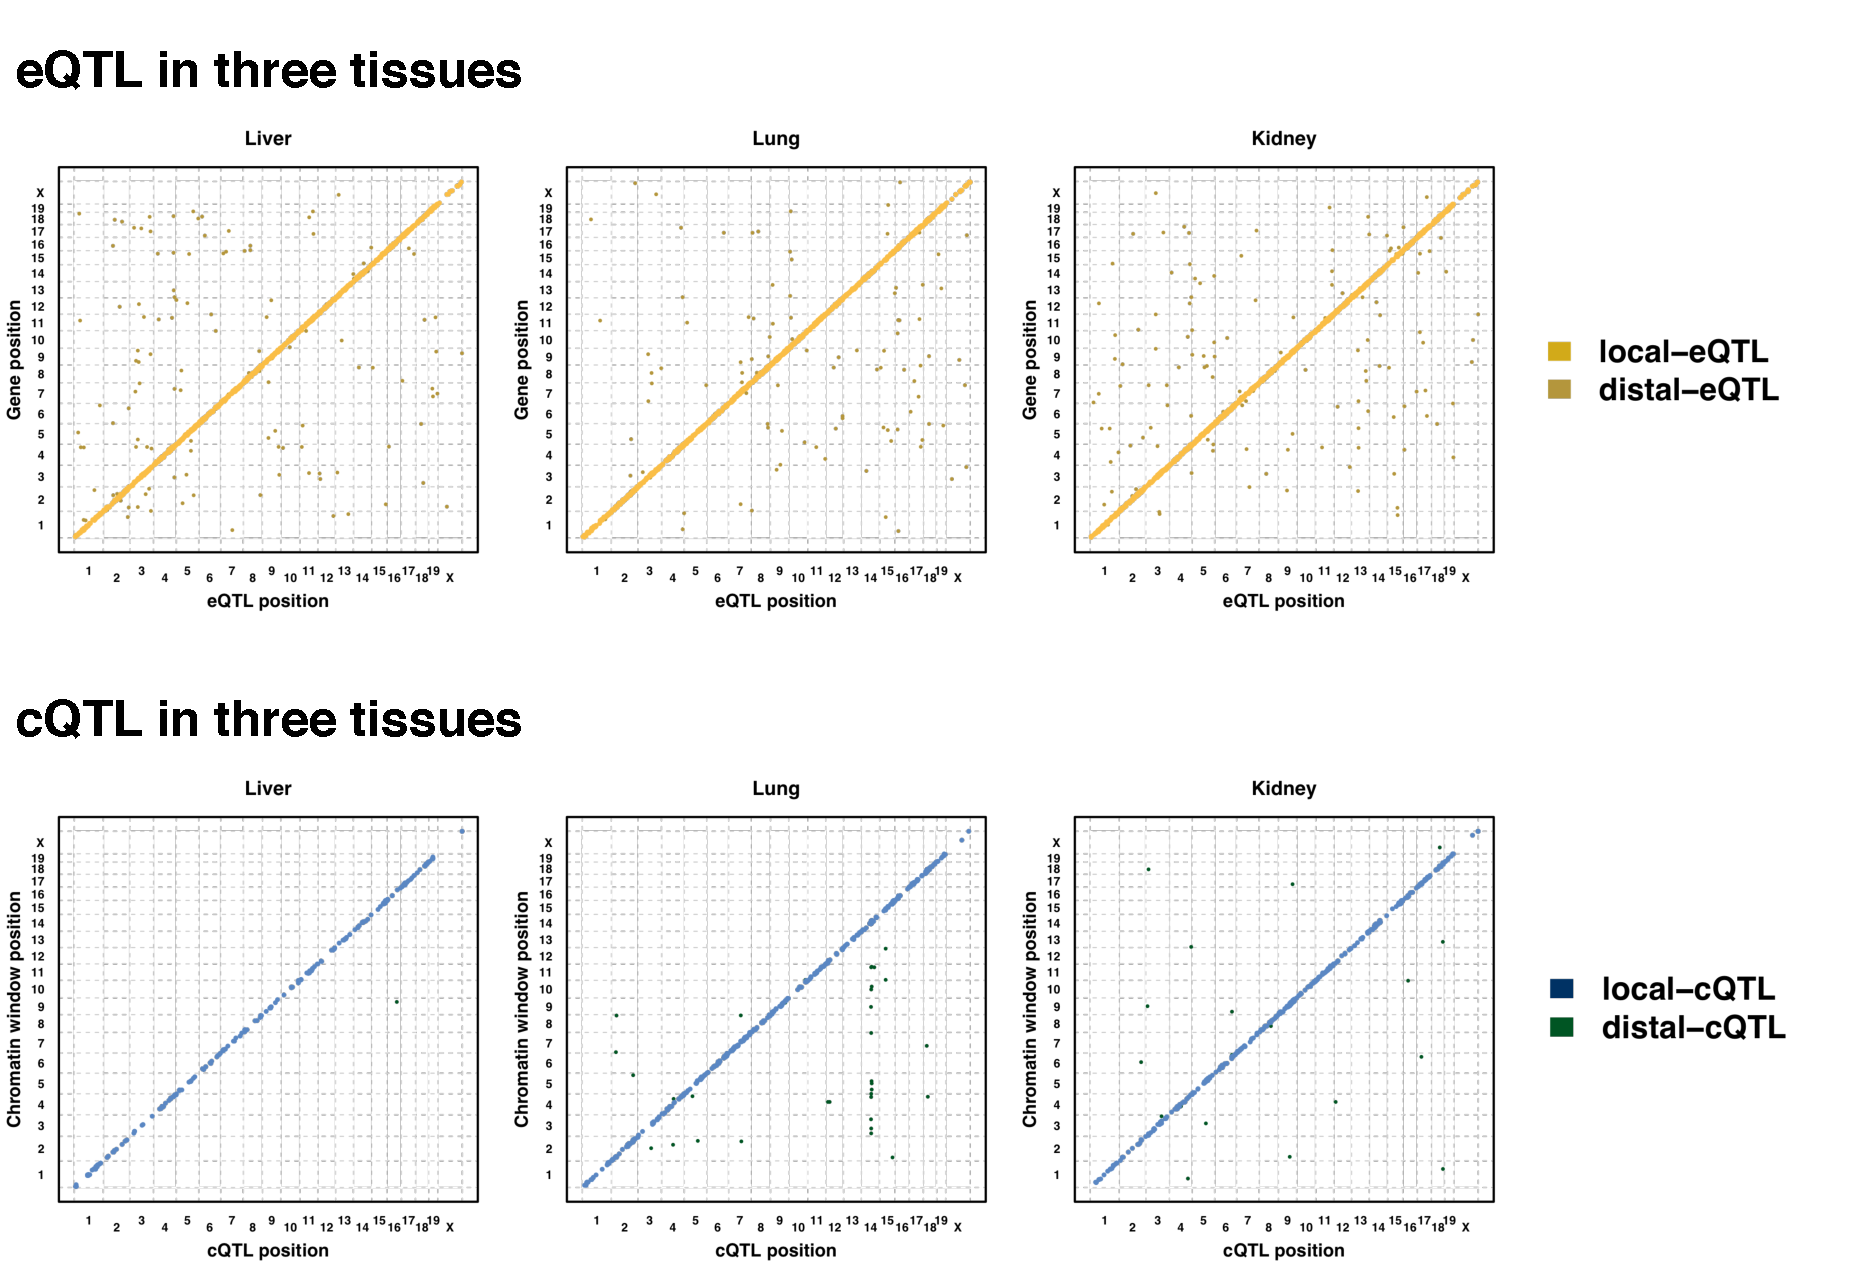
\includegraphics[width=\textwidth, trim={0in 0in 0in 0in}, clip]{figs/qtl_map_main.pdf}
\caption{\textbf{Detected QTL are largely local for both gene expression (A) and chromatin accessibility (B).} Detected QTL from Analysis G (multi-stage FDR) and Analysis L (genome-wide and chromosome-wide) are included, excluding intra-chromosomal distal-QTL detected through Analysis LC. The y-axis represents the genomic position of the gene or chromatin site, and the x-axis represents the genomic position of the QTL. Local-QTL appear as dots along the diagonal, and distal-QTL off of it.
\label{fig:grid_plot}}
\end{figure*}

\subsection{Tissue-specific chromatin QTL}

To determine genetic effects on chromatin structure, genomic regions were divided into $\sim$300 base pair windows, and used in chromatin accessibility QTL (cQTL) analysis with the same scopes of analysis used with eQTL. We tested 11448, 24426, and 17918 chromatin regions in liver, lung, and kidney, respectively. The overlap in chromatin windows across tissues is described in \textbf{Figure \ref{fig:upset_genes_chromatin}B}. Overall, there were substantially fewer cQTL detected compared to eQTL for all tissues (\textbf{Figure \ref{fig:grid_plot}B}; \textbf{Table \ref{tab:cqtl_mapping}}). As with eQTL, cQTL are more likely to be local (66 - 94.1\% for Analysis G; 75 - 90\% for Analysis LC).

\subsection{QTL effect sizes}

\GKinline{We estimated the effect size for each detected QTL. The effect size estimates should not be over-interpreted, as the Beavis effect, \ie QTL effect size inflation, on a sample of 47 strains is expected to be biased upward \citep{Keele2019}; however the estimates can be used to compare QTL detected by different methods.}
%\WV{}{Add one sentence caveat about the Beavis effect, citing \citet{Keele2019}.}
% by two methods (see \textbf{Tables XX}), either the coefficient of determination ($R^{2}$) for the fixed effect fitting of the QTL term (\textbf{Methods}; Eq \ref{eq:effect_size}) or as the proportion of variance explained based on the variance component estimate from a random effect fitting of the QTL term (\textbf{Methods}; Eq \ref{eq:effect_size_ranef}). We primarily report results from the fixed effect approach because the estimates were largely consistent with plausible QTL effect sizes given the size of the study, outlined in \cite{Keele2019}, namely we were not well-powered to detect QTL with effect sizes < 50\% at genome-wide significance. 
\GKinline{As expected, Analysis G detected QTL with large effects (\textbf{Figure \ref{fig:qtl_effect_sizes_by_method}}, red dots). The local-focused Analyses LC and L had greater power to detect local-QTL of smaller effect (\textbf{Figure \ref{fig:qtl_effect_sizes_by_method}}, gray and blue dots). Distal-QTL discovered with the multi-stage mapping procedure (Analysis G; q-value < 0.1) were detected for $\leq$ 1.6\% of tested genes (\textbf{Table \ref{tab:eqtl_mapping}}) and $\leq$ 0.2\% of tested chromatin windows (\textbf{Table \ref{tab:cqtl_mapping}}), shown in \textbf{Figure \ref{fig:grid_plot}} as the dark colored dots off the diagonals. Consistent with previous studies [\eg, \citet{Chick2016}], distal-QTL have weaker effects than local-QTL (\textbf{Figure \ref{fig:qtl_effect_sizes_local_v_distal}}).} 
\GKinline{For both Analysis G and LC, between two to three times as many local-eQTL are detected compared with
%\WV{with}{\st{to}. Throughout: note that ``compare to'' is a synonym for ``liken to'', \eg, ``shall I compare thee to a Summer's day''; ``compare with'' is to evaluate the relative merits/similarities/differences. In this MS, you almost always mean compare with.} 
distal-eQTL, likely reflecting these stronger effects. A similar dynamic of local to distal signal is seen for cQTL, though the greatly reduced numbers result in less stable ratios across the tissues.}
%For some distal-eQTL, the effect sizes estimated through random effects models approach zero, potentially resulting from highly influential data points in the fixed effect regression procedure and are thus likely to be false positives (\textbf{Figure \ref{fig:qtl_effect_size_fixefvsranef}}). 
%Consistent with eQTL, the effect sizes of local-cQTL are on average higher than distal-cQTL (\textbf{Figure \ref{fig:qtl_effect_sizes_strict} [bottom]}), likely contributing to the to the small number of detected distal-cQTL. cQTL with low effect size are primarily distal-cQTL and may represent false positives. 

\subsubsection{\GKinline{Local-QTL are stronger than distal.}}
%\WV{To assess whether our distance-based classification of intra-chromosomal local- vs distal-eQTL was reasonable, we plotted the statistical association for all intra-chromosomal eQTL from Method 1 (\textbf{Figure \ref{fig:genomewide_dist} [top]}) and the less stringent Method 2 (\textbf{Figure \ref{fig:chrwide_dist} [top]}).}{Make clearer what you are trying to do and why.} 
\GKinline{For QTL detected on the local chromosome (intra-chromosomal), the strongest associations were observed within 10Mb of the gene TSS or chromatin window midpoint (\textbf{Figure \ref{fig:dist_all}}). Intra-chromosomal distal-QTL had reduced statistical significance, more consistent with inter-chromosomal distal-QTL.} 
%\GKinline{Consistent with these effect size dynamics, most intra-chromosomal QTL are local, and their significance of association than the distal intra-chromosomal QTL (Method 1; \textbf{Figure \ref{fig:genomewide_dist}} and Method 2; \textbf{Figure \ref{fig:chrwide_dist}}).} Similar to local-eQTL, but to a lesser extent, the majority of chromatin windows with local-cQTL were only observed in one tissue (\textbf{Figure \ref{fig:upset_eqtl_cqtl} [right]}).

%In addition to finding that the majority are local-eQTL, we see a drastic reduction in the strength of the statistical association outside of the defined local region. This suggests that intra-chromosomal distal-eQTL are more similar to inter-chromosomal distal-eQTL than local-eQTL, and that our 10Mb boundaries are appropriate. 

\subsubsection{\GKinline{CAST and PWK drive QTL with extreme haplotype effects.}}
\GKinline{Founder haplotype effects were estimated for all QTL. Consistent with previous studies [\eg \citet{Aylor2011}], the CAST and PWK haplotypes tended to have more extreme effects than the classical inbred strains. This pattern was observed for both local and distal-eQTL (\textbf{Figure \ref{fig:qtl_effects_abs}A}) and local-cQTL, whereas the numbers of detected distal-cQTL were too low to produce clear trends (\textbf{Figure \ref{fig:qtl_effects_abs} B}).}

%Again we found that the CAST and PWK haplotypes have more extreme effects than the other strains for local-cQTL, though the pattern is less pronounced than with local-eQTL, likely due to the reduced number of cQTL (\textbf{Figure \ref{fig:cqtl_effects_abs}}). The numbers of detected distal-cQTL were low, and no clear trends are obvious.

\section{\GKinline{QTL paired across multiple tissues}}

%\WV{}{Break up this section with headlines.}

For a given trait, QTL from different tissues were paired based on co-localizing to approximately the same genomic region. For local-QTL, both had to be within the local window, defined at 10Mb around the gene TSS, resulting in a maximum distance of 20Mb between QTL. For distal-eQTL, both had to be within 10Mb of each other. 
For local-eQTL, we detected 761 (liver/lung), 1206 (liver/kidney), and 1025 (lung/kidney) pairs. For distal-eQTL, we detected 61 (liver/lung), 120 (liver/kidney), and 59 (lung/kidney) pairs. For cQTL, the vast majority of pairs were local, with 55 (liver/lung), 56 (liver/kidney), and 142 (lung/kidney). Only 4 distal-cQTL pairs were observed, all between lung and kidney. The effect sizes of paired QTL vary across tissues, though they were significantly correlated (\textbf{Figure \ref{fig:qtl_effect_size_comparison}}).

\subsubsection{\GKinline{Multi-tissue QTL pairs share similar founder effects across tissues.}}
The correlation between the founder haplotype effects for pairs of QTL were calculated (FDR $\le 0.1$; \textbf{Figures \ref{fig:qtl_pair_histograms}}), revealing positive correlations for 345 (liver/lung), 623 (liver/kidney), and 498 (lung/kidney) local-eQTL pairs and 21 (liver/lung), 34 (liver/kidney), and 16 (lung/kidney) distal-eQTL pairs. Highly correlated QTL pairs were highly proximal to each other (\textbf{Figure \ref{fig:qtl_cor_by_distance_comparison}}), suggesting that the underlying causal variants are the same or linked. For local-cQTL, 47 (liver/lung), 48 (liver/kidney), and 118 (lung/kidney) positively correlated pairs were identified. The correlations between distal-cQTLs were not formally tested because there were only four pairs; however, three of the four pairs had correlations greater than 0.5. No negatively correlated QTL pairs were detected, after accounting for multiple testing.

\begin{figure*}[h!]
\renewcommand{\familydefault}{\sfdefault}\normalfont
\centering
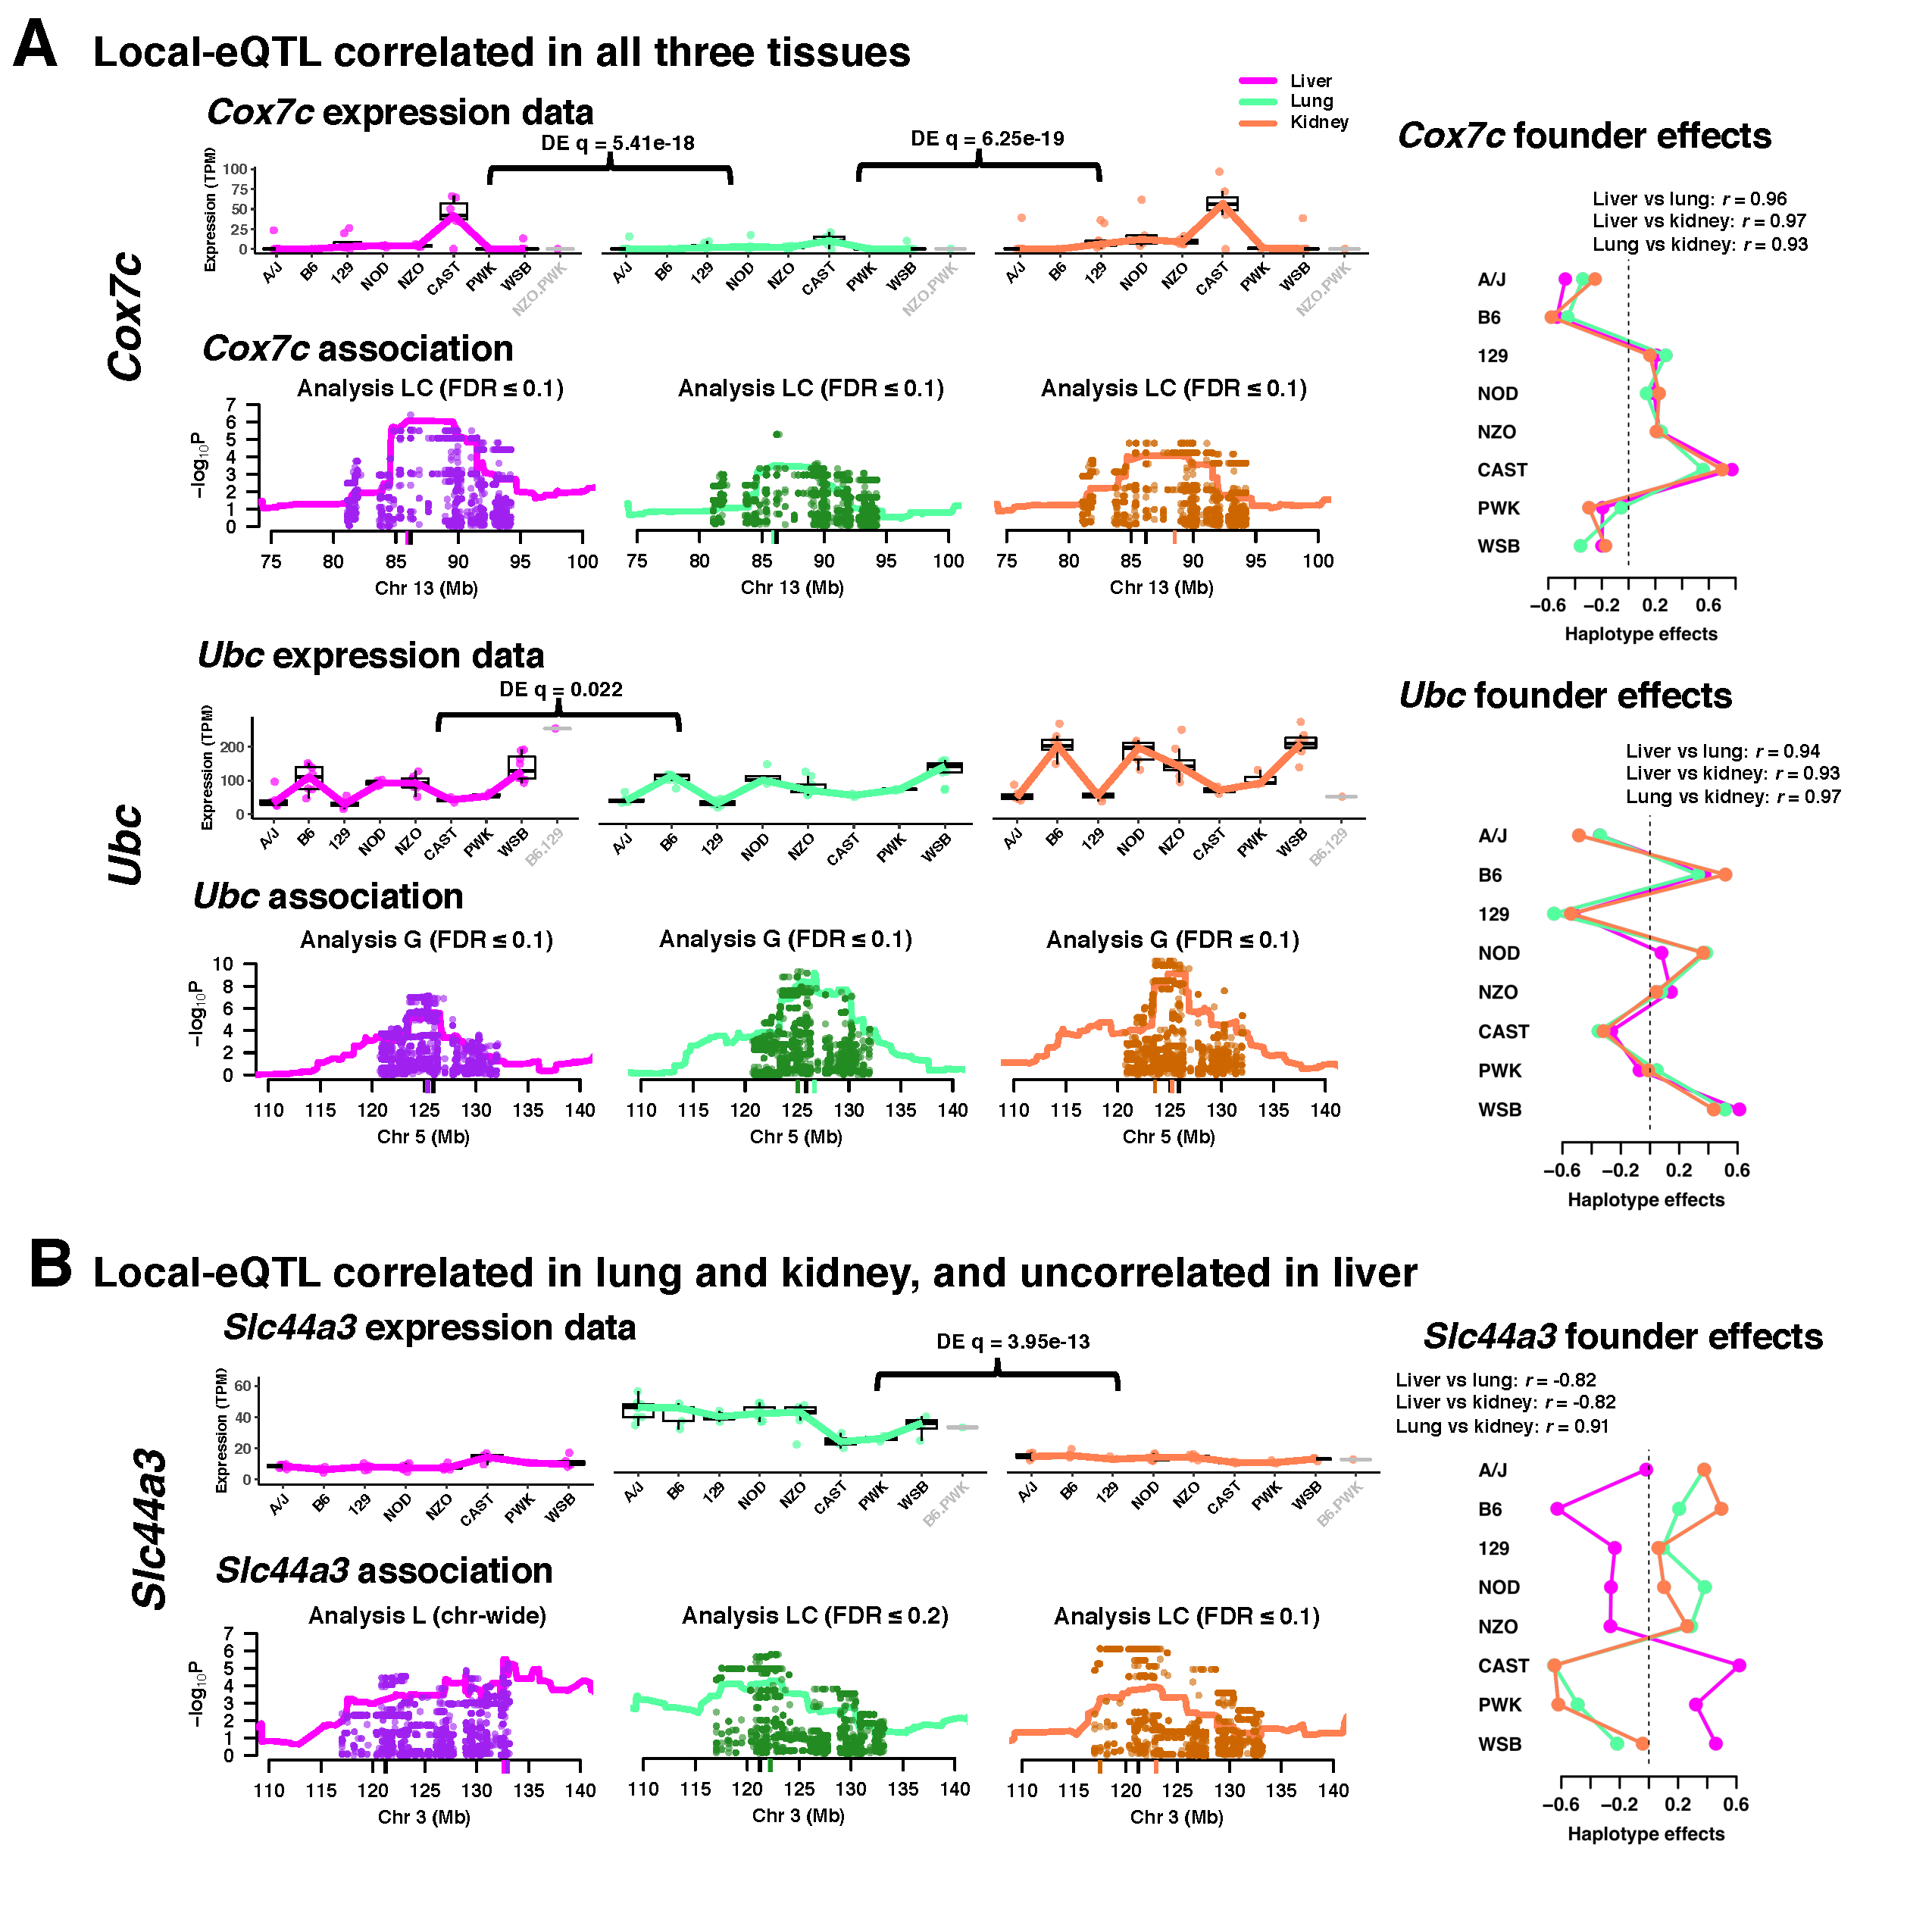
\includegraphics[width=0.9\textwidth, trim={0in 0.5in 0in 0in}, clip]{figs/correlated_local_eqtl.pdf}
\caption{\textbf{Examples of genes with local-eQTL observed in all three tissues.} \textit{Cox7c} and \textit{Ubc} possess local-eQTL with highly correlated founder alllele effects across all three tissues, supportive of shared causal origin (A). \textit{Slc44a3} has a more complicated pattern of local-eQTL founder effects across the tissues, with correlated effects shared between lung and kidney, and transgressive effects in the liver eQTL by comparison, consistent with distinct casual variants comparing liver to lung and kidney. (B). For each gene, the expression data are plotted with boxplots based on most likely founder haplotype pair (diplotype), and differential expression between tissues is highlighted. The haplotype association for each tissue is also included near the gene TSS with variant association overlaid. The most statistically rigorous method to detect the QTL is also included. The black tick represents the gene TSS and the colored ticks represent haplotype and variant peaks. Founder effects estimated as constrained BLUPs are also included with their pairwise correlations. Estimated effects were generally consistent with the expression data.\label{fig:correlated_local_eqtl}}
\end{figure*}

%\subsection{Genes with correlated local-eQTL: \textit{Cox7c} and \textit{Ubc}}

\subsubsection{\GKinline{\textit{Cox7c} and \textit{Ubc}: Consistent haplotype effects for multi-tissue local-eQTL.}}
Cytochrome c oxidase subunit 7C (\textit{Cox7c}) and ubiquitin C (\textit{Ubc}) are examples of genes that possess local-eQTL with highly correlated effects in all three tissues (\textbf{Figure \ref{fig:correlated_local_eqtl}A}).
For \textit{Cox7c} local-eQTL were driven by high expression when the CAST haplotype was present, intermediate expression with 129, NOD, and NZO haplotypes, and low expression with A/J, B6, PWK, and WSB haplotypes. The \textit{Ubc} local-eQTL were driven by high expression with the B6, NOD, NZO, and WSB haploytpes. Though the founder effects are consistent across tissues for both genes, we note that expression of \textit{Cox7c} was significantly higher in liver compared to both lung ($q = \num{5.41e-18}$) and kidney ($q = \num{6.25e-19}$), and for \textit{Ubc}, expression in liver and lung were considered significantly differential ($q = 0.022$). 

%The haplotype and variant associations in the local region match closely for all tissues for both \textit{Cox7c} and \textit{Ubc}. Though all the \textit{Ubc} local-eQTL were detected with the most stringent Method 1, the \textit{Cox7c} local-eQTL were detected with the more lenient Method 2.

%\subsection{Genes with uncorrelated local-eQTL: \textit{Slc44a3} and \textit{Pik3c2g}}

\begin{figure*}[h]
\renewcommand{\familydefault}{\sfdefault}\normalfont
\centering
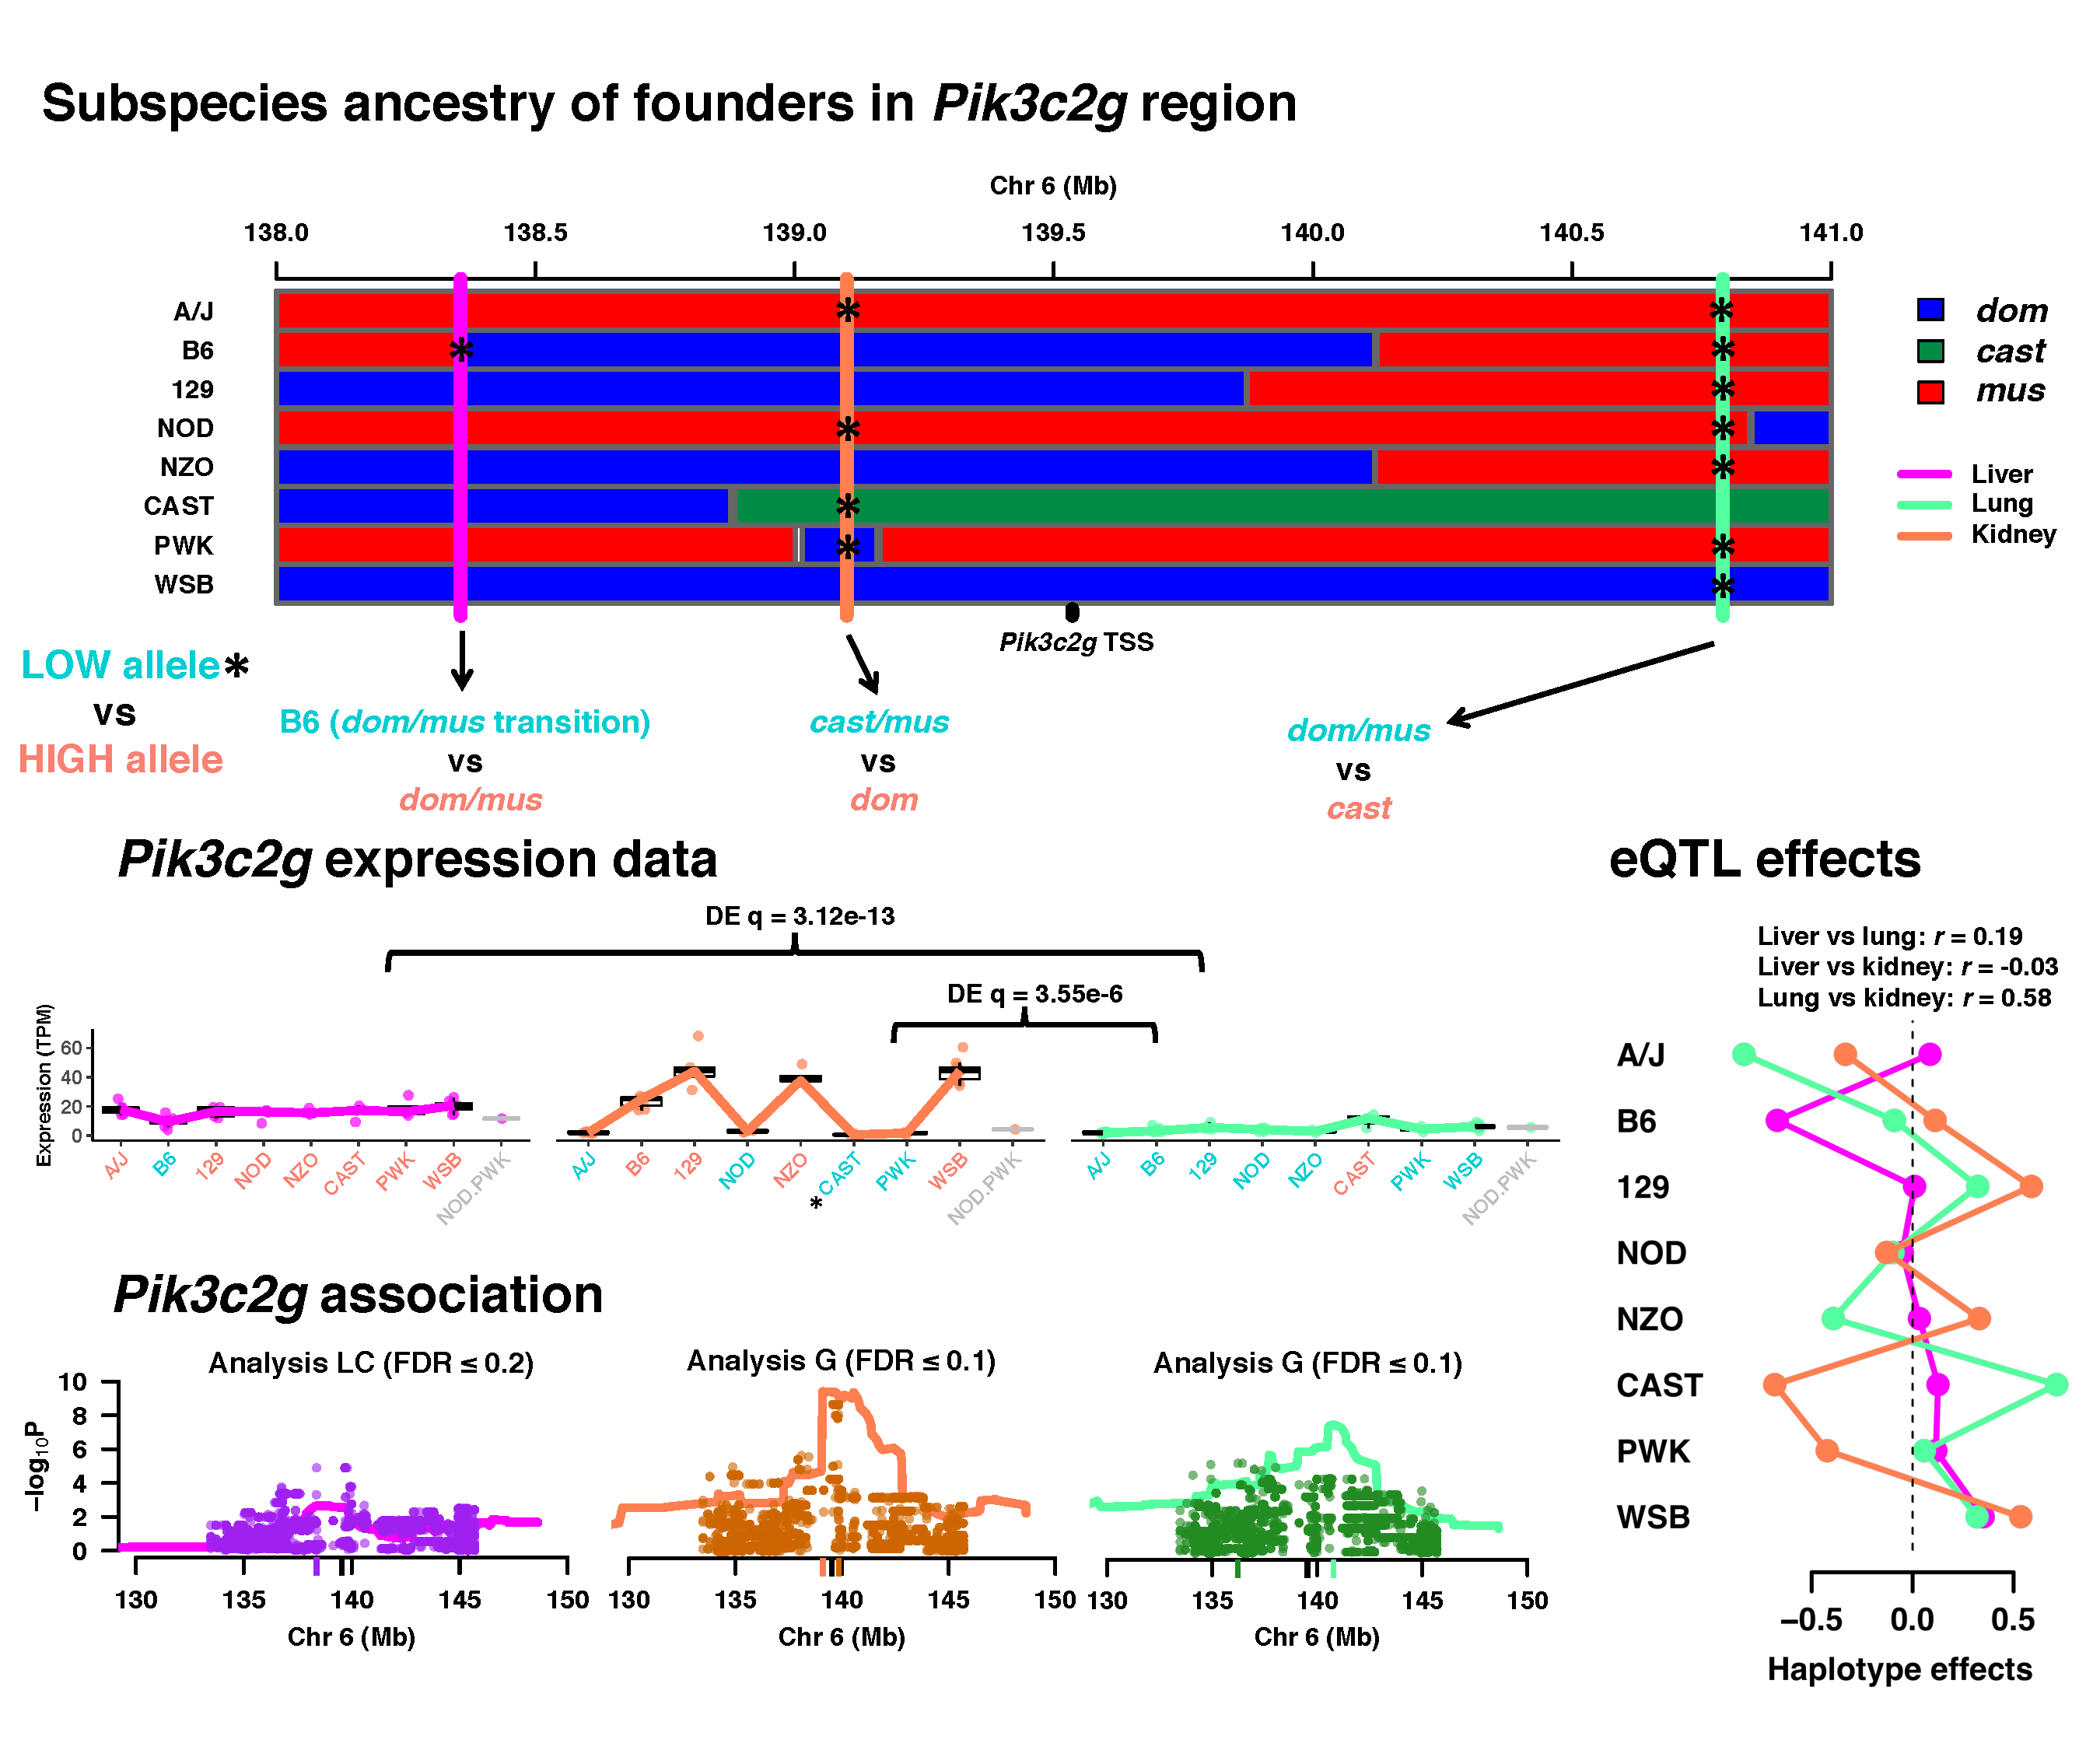
\includegraphics[width=0.9\textwidth, trim={0in 0.5in 0in 0in}, clip]{figs/pik3c2g_example.pdf}
\caption{\textbf{\textit{Pik3c2g} possesses tissue-specific local-eQTL.} Local-eQTL for \textit{Pik3c2g} are detected in all three tissues in the 3Mb region surrounding its TSS. The genomes of the CC founders can be simplified in terms of contributions from three subspecies lineages of \textit{M. musculus}: \textit{dom} (blue), \textit{cast} (green), and \textit{mus} (red). The effects of each local-eQTL matched the subspecies contributions near the eQTL coordinates, with low subspecies alleles colored teal and high alleles colored salmon, consistent with local-eQTL for \textit{Pik3c2g} being distinct and tissue-specific. The gene expression data are represented as boxplots, categorized based on most likely diplotype at the eQTL for each CC strain. Haplotype and variants associations are included for each tissue, with the black tick representing the \textit{Pik3c2g} TSS and colored ticks representing haplotype and variant peaks. The most rigorous procedure to detect each QTL is reported. Founder effects, estimated as constrained BLUPs, were consistent with the expression data, and uncorrelated across the tissues.\label{fig:pik3c2g}}
\end{figure*}

\subsubsection{\GKinline{\textit{Slc44a3} and \textit{Pik3c2g}: Tissue-specific local-eQTL.}}
QTL pairs that are uncorrelated potentially represent distinct tissue-specific QTL where genetic variants influence gene expression or chromatin accessibility in a tissue-specific pattern. For example, the solute carrier family 44, member 3 (\textit{Slc44a3}) gene has correlated local-eQTL effects in lung and kidney, but unique effects in liver (\textbf{Figure \ref{fig:correlated_local_eqtl}B}). Notably, the effects in liver are anti-correlated with the effects in lung and kidney, suggesting the liver eQTL could be transgressive \citep{Rieseberg1999} to the eQTL in lung and kidney, whereby the effects of the founder haplotypes are reversed. For \textit{Slc44a3}, CAST, PWK, and WSB haplotypes result in higher expression in liver, but lower expression in lung and kidney. 
The local-eQTL for \textit{Slc44a3} were more similar in location in lung and kidney, whereas the liver eQTL was more distal to the gene TSS. Overall, the expression data, estimated effects, and patterns of association are consistent with lung and kidney sharing a causal local-eQTL, and liver possessing a unique one. 
%The lung eQTL was detected with the highly lenient Method 2 (FDR $\leq$ 0.2) and the kidney eQTL with the less lenient Method 2 (FDR $\leq$ 0.1). The liver eQTL was detected with the lenient Method 3 (chromosome-wide). 

Another example is phosphatidylinositol-4-phosphate 3-kinase catalytic subunit type 2 gamma (\textit{Pik3c2g}), a gene of interest for diabetes-related traits \citep{Braccini2015}. \textit{Pik3c2g} has local-eQTL in all three tissues but that are all uncorrelated (\textbf{Figure \ref{fig:pik3c2g}}). Expression of \textit{Pik3c2g} varies at statistically significant levels for liver versus lung ($q = \num{3.12e-13}$) and lung versus kidney ($q = \num{3.55e-6}$). The presence of tissue-specific local-eQTL is further supported by the \textit{Mus musculus} lineages in the genomic region local to \textit{Pik3c2g}. The CC founder strains all possess contributions from three subspecies of \textit{M. musculus}: \textit{domesticus} (\textit{dom}), \textit{castaneus}, (\textit{cast}), and \textit{musculus} (\textit{mus}) \citep{Yang2011}. \cite{Crowley2015} found that allele-specific gene expression in mice descended from the CC founders often followed patterns that matched the subspecies inheritance at the gene regions.
In lung, the CAST haplotype, which represents the \textit{cast} subspecies lineage at the locus, results in higher expression, consistent with a \textit{cast} versus \textit{dom}/\textit{mus} allelic series. In kidney, the B6, 129, NZO, and WSB haplotypes result in higher expression, whereas A/J, NOD, CAST, and PWK haplotypes show almost no expression, mostly consistent with a \textit{dom} versus \textit{cast}/\textit{mus} allelic series. The PWK founder has a small \textit{dom} haplotype block at the QTL peak in a broader region that is largely \textit{mus}. The expression data are highly consistent with PWK having the \textit{mus} allele, suggesting that the causal variant is located in a nearby region, supported by the variant association. Notably, the B6 haplotype confers an intermediate level of expression to the other founders that possess \textit{dom} inheritance, representing a potentially multi-allelic QTL that haplotype association can better identify in comparison to bi-allelic variant association. In liver, the B6 haplotype resulted in lower expression. The B6 founder does not have a unique subspecies lineage at the locus, but instead possesses a recombination event between \textit{dom} and \textit{mus}, potentially disrupting the local regulation specific to each subspecies lineage and explaining the reduced expression.

%\subsection{Genes with distal-QTL observed across tissues: \textit{Akr1e1}, \textit{Per2}, and \textit{Rnf13}}

\begin{figure*}[h!]
\renewcommand{\familydefault}{\sfdefault}\normalfont
\centering
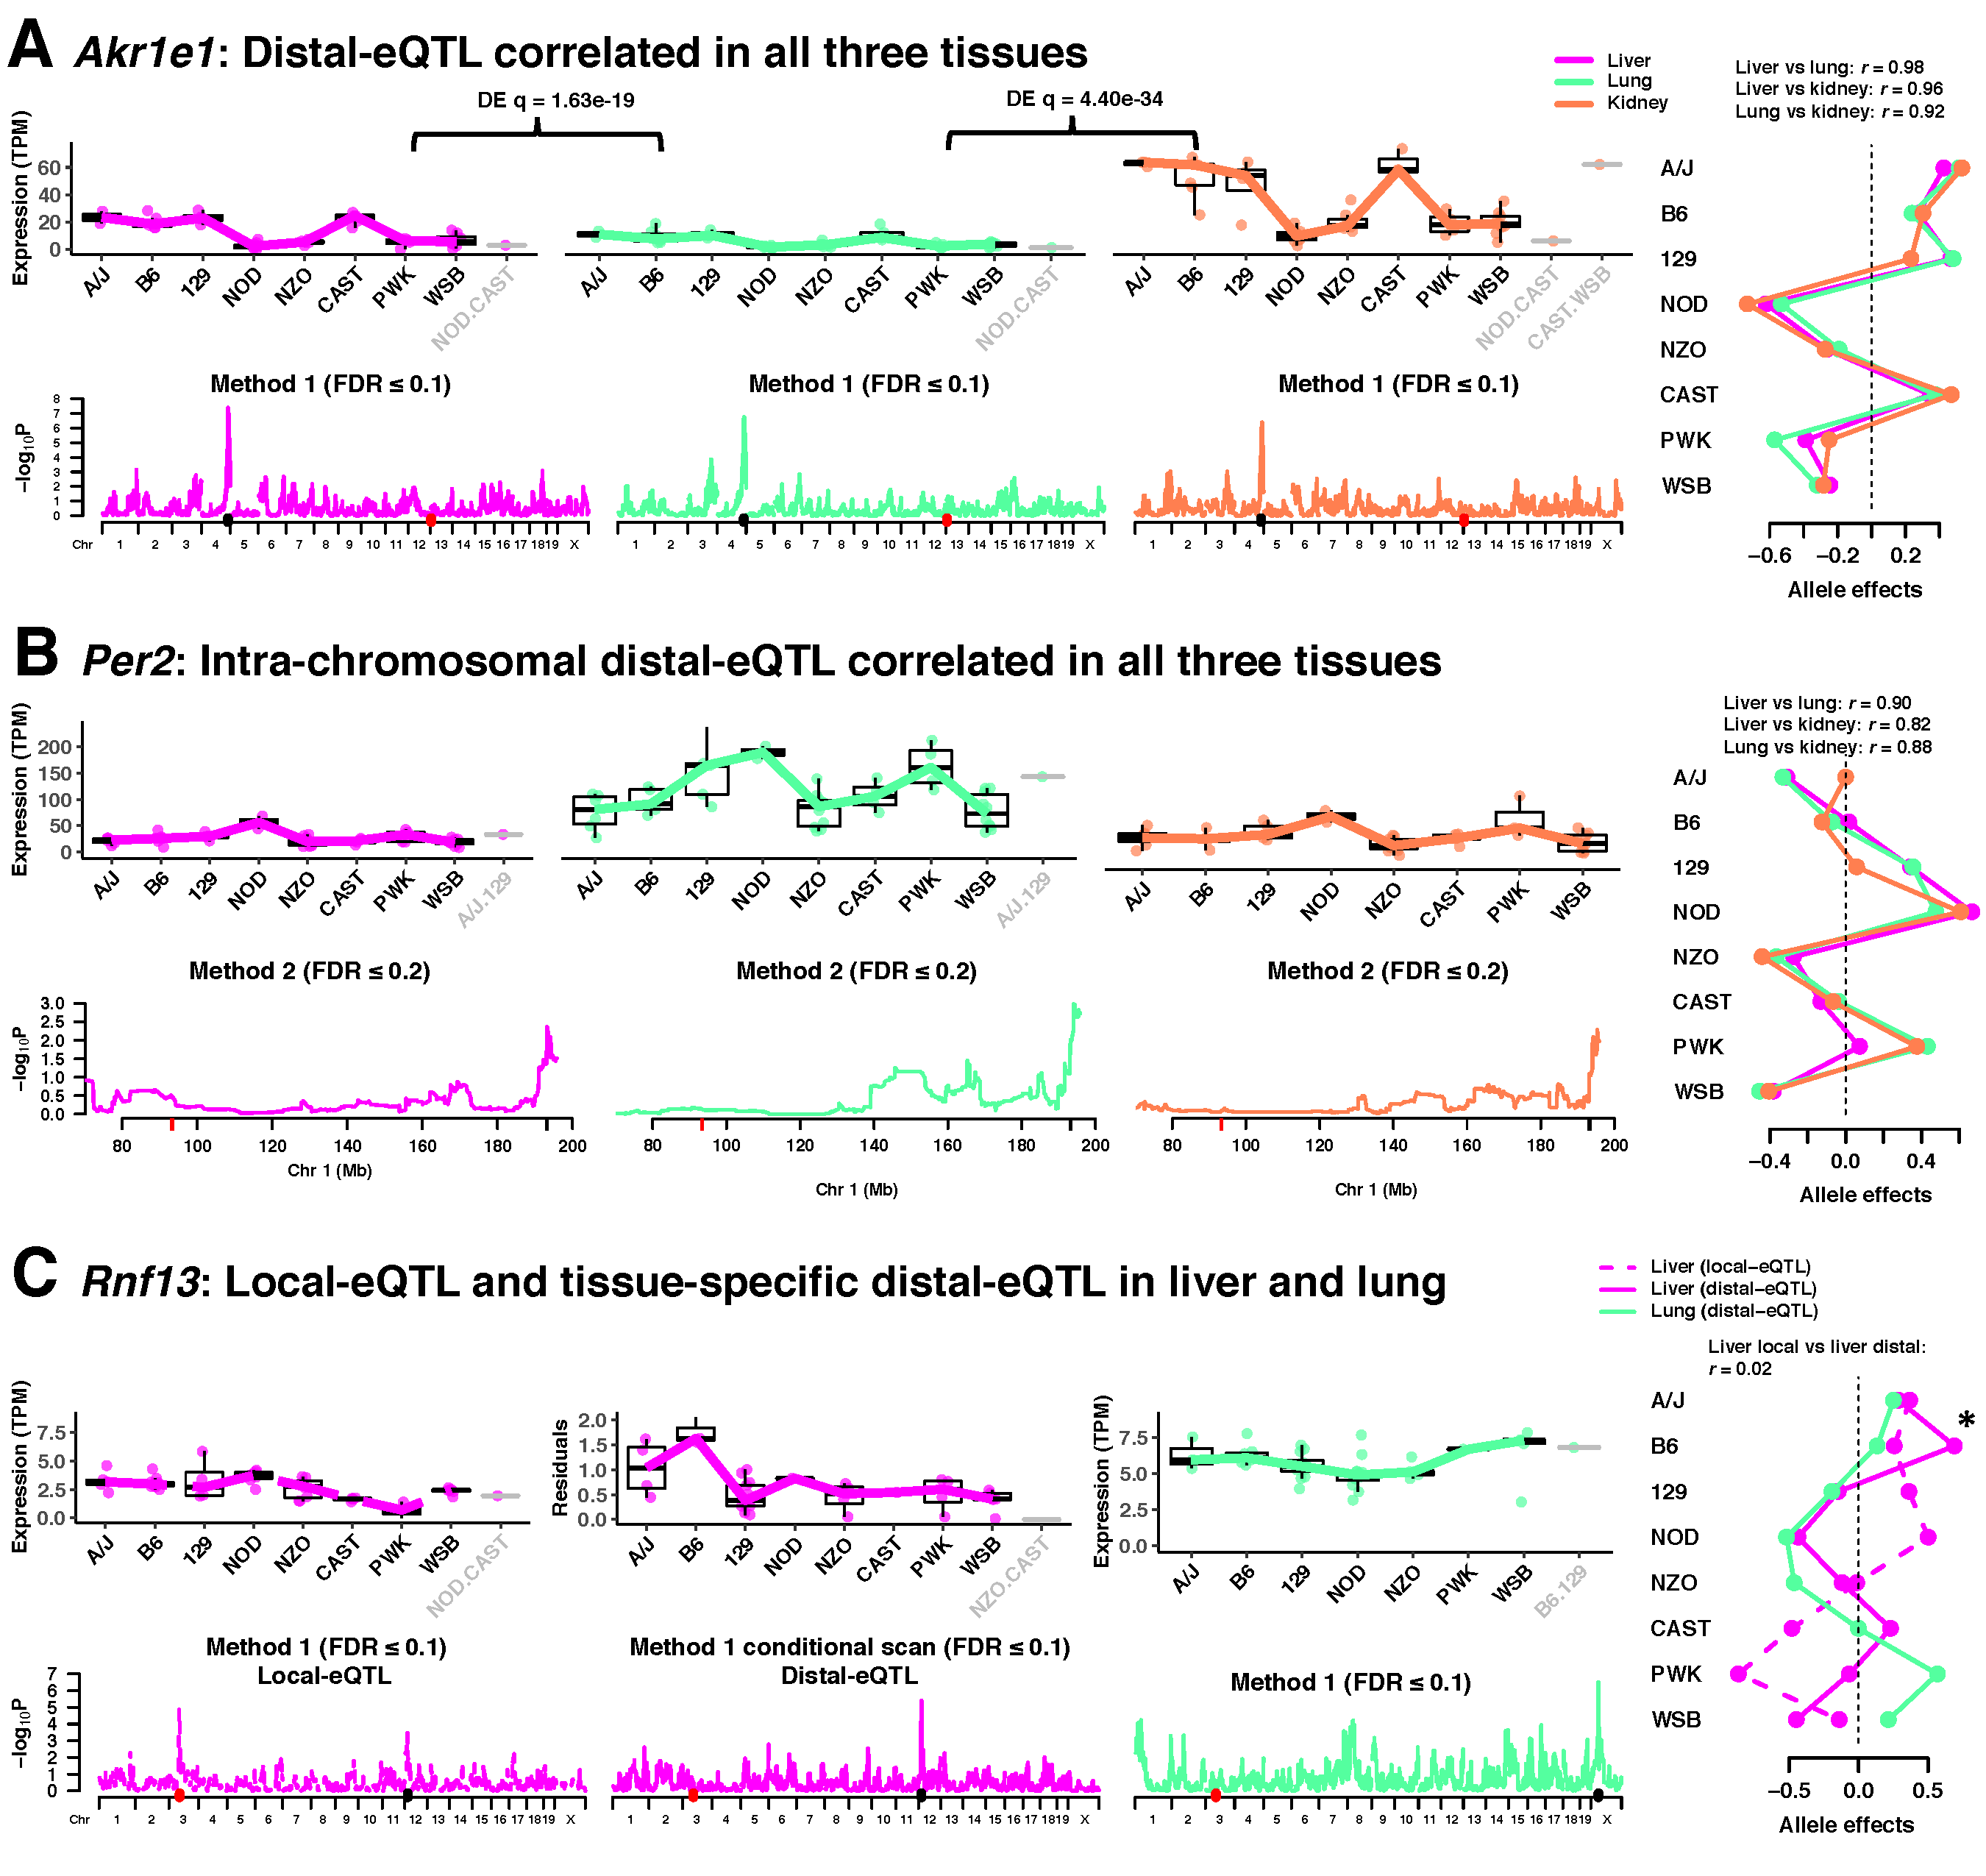
\includegraphics[width=0.9\textwidth, trim={0in 0in 0in 0in}, clip]{figs/correlated_distal_eqtl.pdf}
\caption{\textbf{Examples of genes with distal-eQTL effect patterns across tissues.} \textit{Akr1e1} has highly significant distal-eQTL detected on chromosome 4 in all three tissues with correlated founder effects (A). \textit{Per2} has intra-chromosomal distal-eQTL leniently detected 100Mb away from the TSS, also with highly correlated founder effects across the tissue, providing further support that the distal-eQTL are real (B). \textit{Rnf13} has a liver-specific distal-eQTL on chromosome 13 detected after conditioning on its local-eQTL on chromosome 2, and a lung-specific distal-eQTL on chromosome X, each with distinct founder effect patterns (C). Expression data are represented as boxplots for most likely diplotype, with differential expression noted when significant. Haplotype associations for each tissue distal-eQTL combination are shown, with the most rigorous statistical procedure for detection reported. Red ticks signify the gene TSS and black ticks represent that eQTL peak. Fit founder effects, estimated as BLUPs, are included, along with the pairwise correlations of the eQTL. The black asterisk marks the high B6 effect that drives the distal-eQTL in liver after conditioning on the local-eQTL for \textit{Rnf13}.
\label{fig:correlated_distal_eqtl}}
\end{figure*}

\begin{figure*}[h]
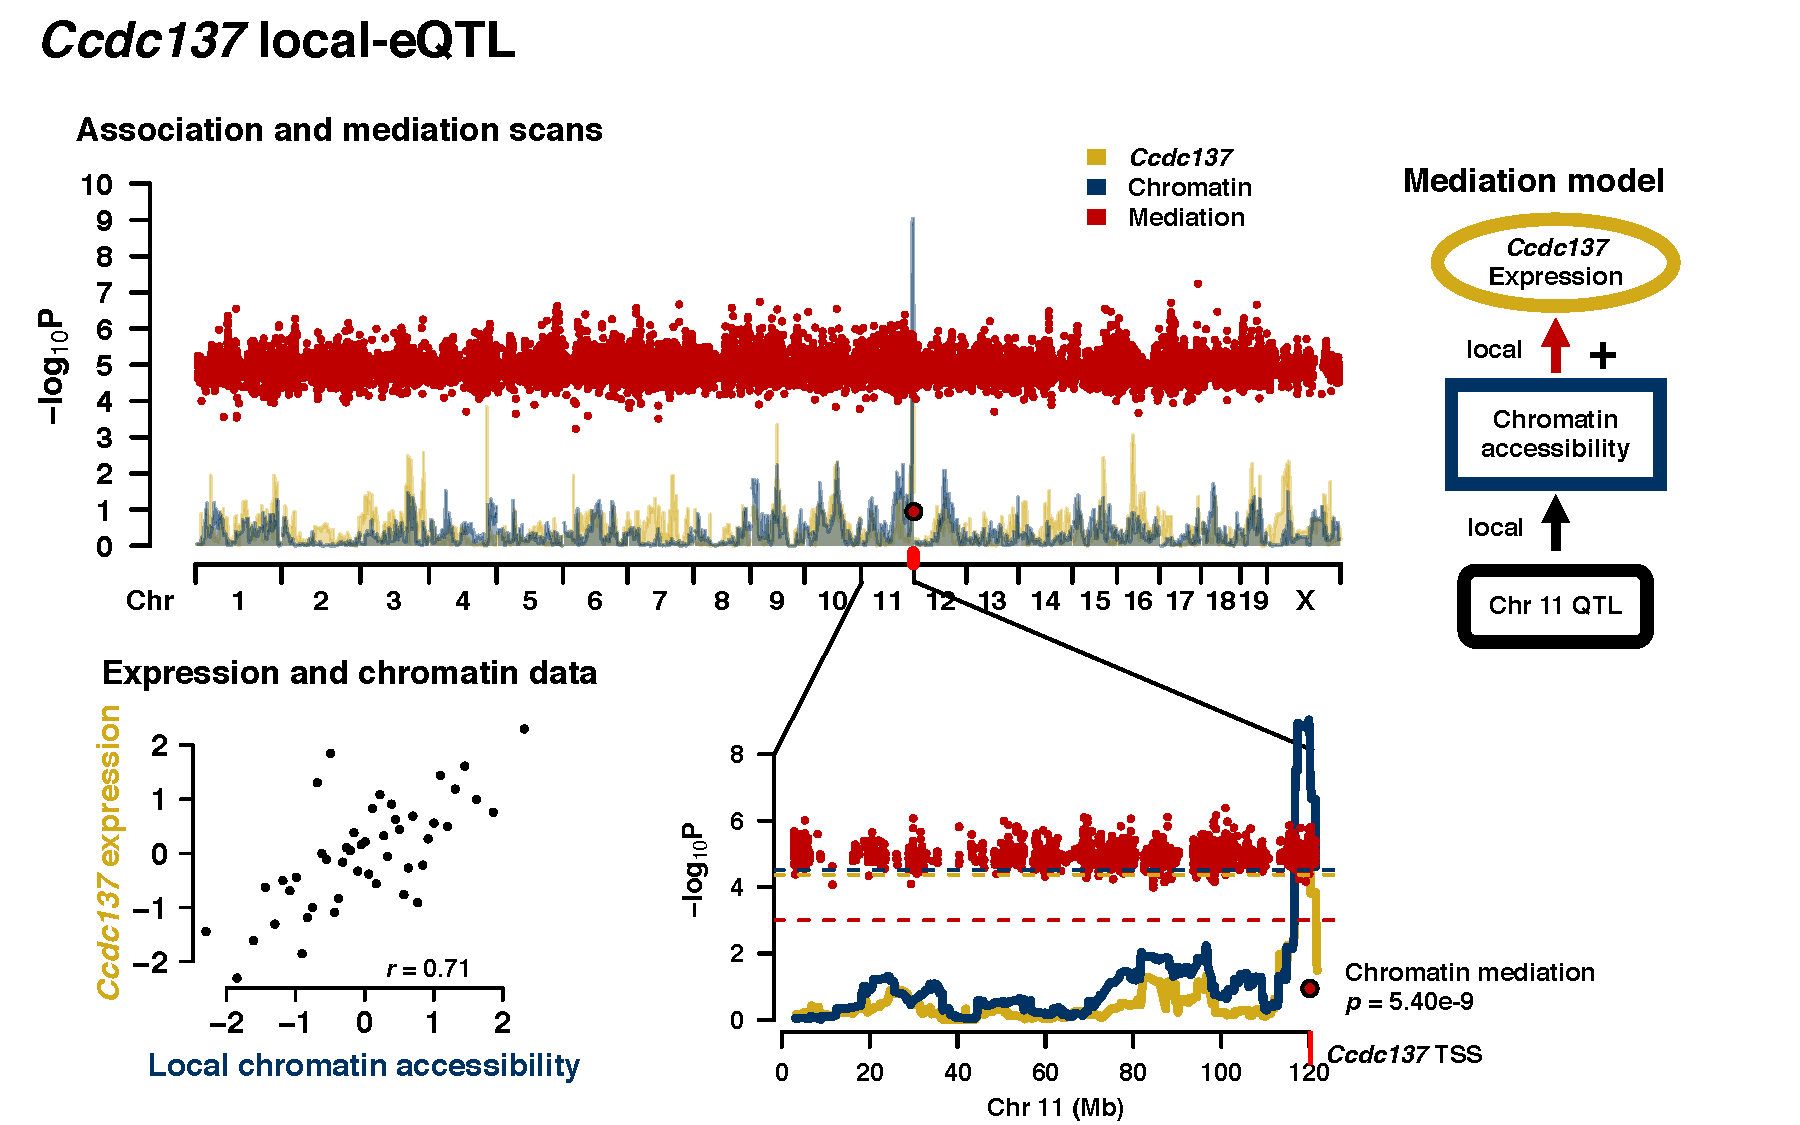
\includegraphics[width=\textwidth, trim={0in 0in 0in 0in}, clip]{figs/ccdc137_mediation.pdf}
\caption{\textbf{\textit{Ccdc137} local-eQTL is mediated by proximal chromatin accessibility.} \textit{Ccdc137} expression and the chromatin accessibility in the proximal region are highly correlated ($r = 0.71$). Genome scans for \textit{Ccdc137} expression (yellow), nearby chromatin accessibility (blue), and chromatin mediation of the \textit{Ccdc137} local-eQTL (red) in lung tissue. The local-eQTL and local-cQTL for the chromatin region at the TSS of \textit{Ccdc137} (red tick) are over-lapping. The steep drop in the statistical association, represented as logP, for the chromatin site in the mediation scan supports chromatin mediation of \textit{Ccdc137} expression, depicted as a simple graph in the topright. The QTL and mediation signals are detected at genome-wide significance. \label{fig:ccdc137_mediation}}
\end{figure*}

\subsubsection{\GKinline{\textit{Akr1e1} and \textit{Per2}: Consistent haplotype effects for multi-tissue distal-eQTL.}}
Founder haplotype effects that correlate across tissues can provide stronger confirmation of distal-QTL, even those with marginal significance. 
%Though fewer distal-QTL were significantly correlated across tissues in comparison to local-QTL (71 to 1,466 for eQTL and 2 to 213), potentially reflecting the reduced power to detect distal-QTL in this study, a number of genes were identified with unique patterns of distal-eQTL over the tissues, shown in \textbf{Figure \ref{fig:correlated_distal_eqtl}}.
For example, the Aldo-keto reductase family 1, member E1 (\textit{Akr1e1}; \textbf{Figure \ref{fig:correlated_distal_eqtl}A}) gene is located on chromosome 13 and had no local-eQTL detected in any of the tissues. Distal-eQTL for \textit{Akr1e1} were detected in all tissues that localize to the same distal region of chromosome 4. The founder haplotype effects of the distal-eQTL are all highly correlated, with A/J, B6, 129, and CAST haplotypes being the more highly expressed. The overall magnitude of expression varies significantly across the tissues, with liver and kidney having significantly higher expression than lung ($q = \num{1.63e-19}$ and $q = \num{4.40e-34}$, respectively).
%The distal-eQTL for \textit{Akr1e1} will be discussed further with the topic of mediation.
%As with local-QTL, correlated distal-eQTL can provide strong evidence that marginally significant QTL are valid. 
Another example is the Period circadian clock 2 (\textit{Per2}; \textbf{Figure \ref{fig:correlated_distal_eqtl}B}) gene, which possesses intra-chromosomal distal-eQTL that are detected in all three tissues that are approximately 100Mb away from its TSS. Despite being detected with the highly lenient Analysis LC (FDR $\leq$ 0.2), the founder haplotype effects are significantly correlated among the tissues, characterized by high expression with the NOD and PWK haplotypes present. Collectively, these findings provide strong validation for the distal-eQTL, which would commonly not even be detected based on tissue-stratified analyses.

\subsubsection{\GKinline{\textit{Rnf13}: Tissue-specific distal-eQTL.}}
QTL analysis in multiple tissues also allows for the detection of tissue-specific distal-QTL. The Ring finger protein 13 (\textit{Rnf13}; \textbf{Figure \ref{fig:correlated_distal_eqtl}C}) gene was lowly expressed in all tissue but with a strong local-eQTL detected in liver. The multi-stage conditional regression approach, conditioning on the local-eQTL, detected a distal-eQTL on chromosome 12. Comparing the residuals after regressing out the local-eQTL and founder haplotype effects suggested that mice with B6 contributions at the distal locus had higher \textit{Rnf13} expression. In lung tissue, a distal-eQTL was detected on the X chromosome with a different haplotype effect pattern, notably high expression when A/J, B6, and PWK haplotypes were present, and low expression with NOD and NZO haplotypes. These examples demonstrate that analyzing multiple tissues can provide greater evidence of distal-QTL, as well as potentially identify tissue-specific genetic regulation.

\section{Mediation of eQTL}

Measurement of gene expression and chromatin accessibility data in the same mice and tissues enables the use of mediation analysis to help elucidate the relationships between genotype, chromatin accessibility, and gene expressions. 
We considered two possible models for the mediation of eQTL effects and assessed the evidence for each in our data.

%We assessed evidence for each of two distinct mediation models of eQTL effects (\textbf{Figure \ref{fig:graph}}):
%1) a model the effect of local-eQTL on gene expression is mediated by proximal chromatin accessibility.
%2) the effect of distal-eQTL on gene expression is mediated through proximal gene expression

\subsection{Chromatin intermediates}
%\WVinline{[results good enough to reword as headline, perhaps with gene names?]}}

In the first mediation model, we assess the extent to which proximal chromatin state acted as a mediator of the effect of local-eQTL (\textbf{Figure \ref{fig:graph}A}). This was tested using an approach adapted from \cite{Chick2016} to detect mediation through chromatin accessibility of local-eQTL detected through Analysis L (genome-wide and chromosome-wide; see \textbf{Appendix C} for greater detail).  

\subsubsection{\GKinline{\textit{Ccdc137} and \textit{Hdhd3}: Local-eQTL driven by local chromatin accessibility}}
Across the three tissues, we found from 13-42 local-eQTL showed evidence of mediation through proximal chromatin accessibility at genome-wide significance, and 35-106 at chromosome-wide significance (\textbf{Table \ref{tab:mediation}}). The coiled-coil domain containing 137 gene (\textit{Ccdc137}) is a strong example of mediation through local chromatin accessibility. \textbf{Figure \ref{fig:ccdc137_mediation}} includes the genome scans that identify local-QTL for \textit{Ccdc137} expression (eQTL) and a proximal chromatin accessibility window (cQTL). 
%The red tick marks the TSS for \textit{Ccdc137}, which is highly proximal to both the eQTL and cQTL. The red dots represent the significance of the eQTL after conditioning on each chromatin region as a mediator. 
A large drop in eQTL significance at the location of the cQTL represents a strong mediation signal. A closer inspection of the region shows that the significance of the eQTL and cQTL are similar but notably stronger for chromatin, as expected by the proposed mediator model. 

Co-localization of eQTL and cQTL is not sufficient for mediation. For both \textit{Hdhd3} in liver (\textbf{Figure \ref{fig:colocalization}A}) and the acyl-Coenzyme A binding domain containing 4 gene (\textit{Acbd4}) in kidney (\textbf{Figure \ref{fig:colocalization}B}), there are local-eQTL with a co-localizing cQTL. Comparing the statistical associations at the genomic locations of the eQTL and cQTL as well as the founder haplotype effects for both the eQTL and cQTL, the correspondence in both is better for \textit{Hdhd3} compared to \textit{Acbd4}. As with \textit{Ccdc137}, a strong mediation signal is detected for \textit{Hdhd3}, indicated by the decrease in the eQTL association when conditioning on the chromatin state. Mediation is not detected for \textit{Abcd4}, which is consistent with the genetic regulation of both gene and chromatin site not stemming from the same causal origin.

\subsection{Gene intermediates} 
%\WVinline{[results good enough to reword as headline, perhaps with gene names?]}}

In the second mediation model, \GKinline{expression levels of genes with genomic coordinates local to distal-eQTL were evaluated as potential mediators}. This was tested using an approach similar to \cite{Keller2018} for distal-eQTL detected through Analysis G. 
%A related mediation model was used to identify genome-wide significant distal-eQTL that are mediated through the expression of proximal genes, as might be expected for a transcription factor with its own local-eQTL (\textbf{Figure \ref{fig:graph} B}). 
\subsubsection{\GKinline{Zinc finger protein intermediates detected for \textit{Ccnyl1}.}}
Eight genes were identified with mediated distal-eQTL (\textbf{Table \ref{tab:exmediation}}). As example, the distal-eQTL of cyclin Y-like 1 (\textit{Ccnyl1}) is mediated by the expression of zinc finger protein 979 (\textit{Zfp979}), a putative transcription factor (\textbf{Figure \ref{fig:ccnyl1_exmediation}}). The founder haplotype effects at the distal-eQTL of \textit{Ccnyl1} are highly correlated with the local-eQTL effects for \textit{Zfp979}, though with a reduction in overall strength, in accordance with the proposed mediation model.

\begin{figure*}[h!]
\renewcommand{\familydefault}{\sfdefault}\normalfont
\centering
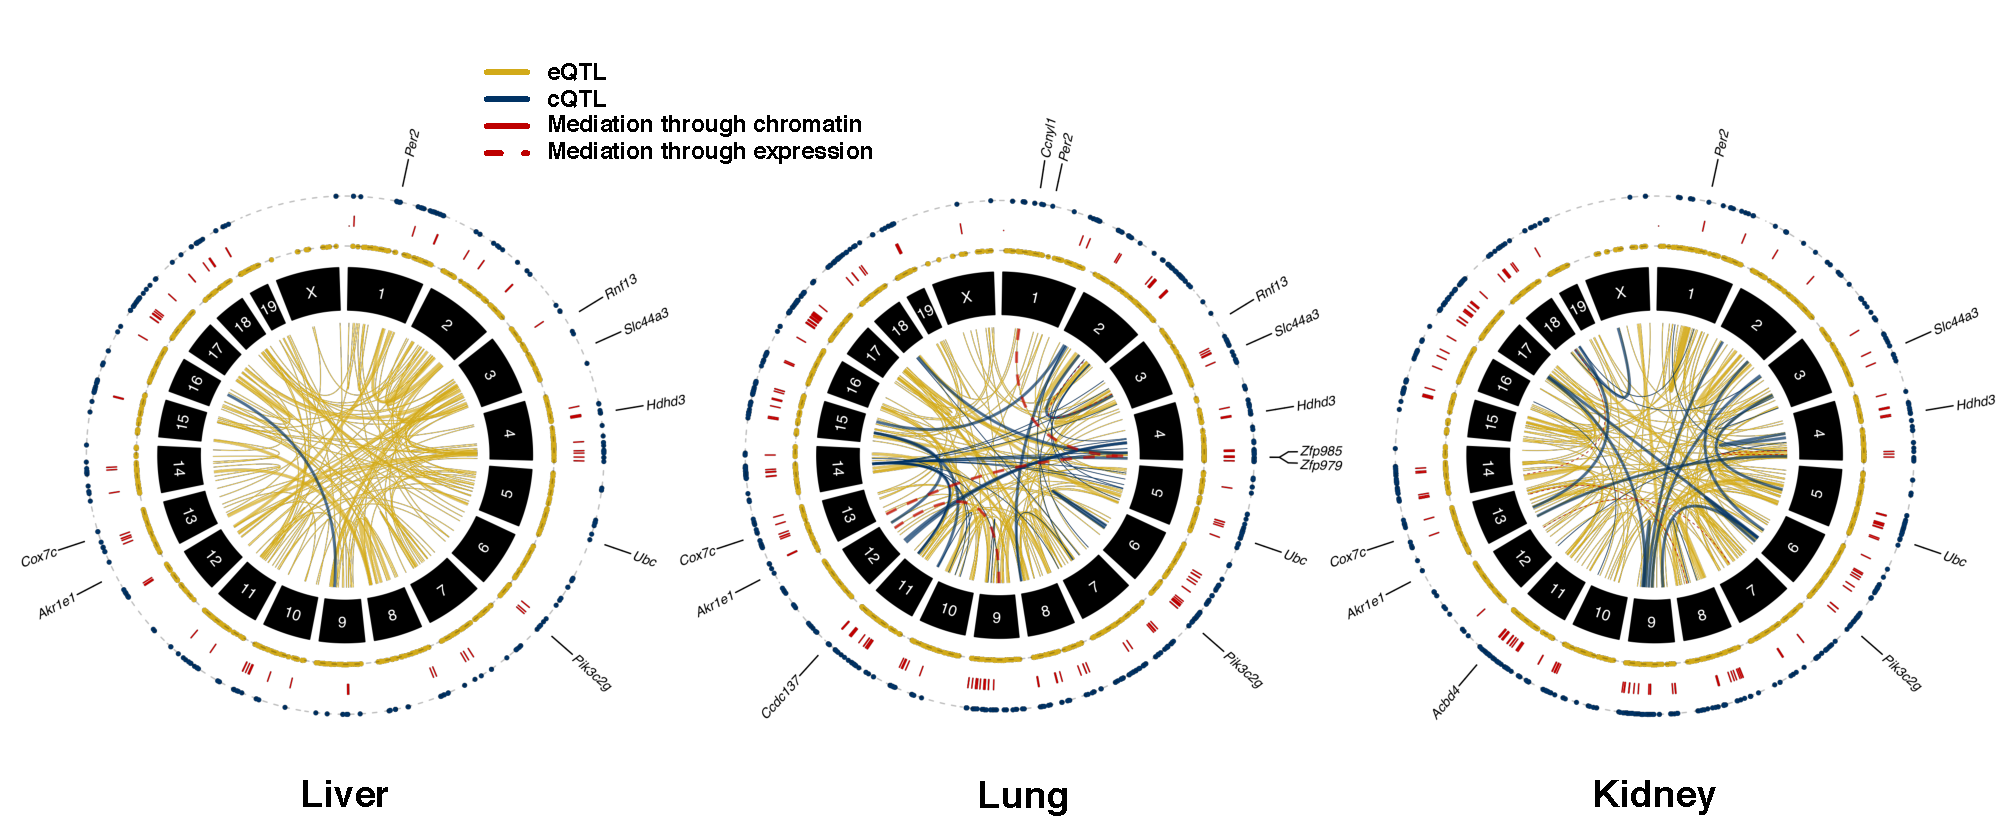
\includegraphics[width=\textwidth, trim={0in 0in 0in 0in}, clip]{figs/circos_over_tissues.pdf}
\caption{\textbf{Summaries of QTL and mediation analyses.} Circos plots of eQTL (yellow), cQTL (blue), and mediation (red) in lung, liver, and kidney. The two outer rings of dots represent local-eQTL and local-cQTL detected by Analysis L at chromosome-wide significance, with red lines between connecting genes and chromatin sites for which chromatin mediation was detected. The inner circle contains connections representing distal-eQTL, distal-cQTL, and gene-gene mediation from Analysis G. Thick lines represent QTL and mediators with permutation-based $p$-value (permP) $< \num{1e-5}$. The detected signals are primarily local, which also tend to be stronger than the observed distal signals. Fewer QTL and mediators are detected in liver tissue. 
%Chromosome 17 has the most concentrated chromatin mediation signal across the three tissues. 
Genes highlighted previously, such as \textit{Akr1e1}, are indicated at their genomic coordinates.
\label{fig:circos_plot}}
\end{figure*}

\subsection{Overview of QTL and mediation analyses}\GK{}{I have moved it up to before \textit{Akr1e1}, and re-written slightly. Moving it up further will require more extensive re-arranging, as I'm currently discussing correlated eQTL effects with examples prior to discussing mediation whatsoever.}
%\WVinline{Move to near the beginning of the results, \ie, BEFORE the deep dive? --- Terry, thoughts?}}
All QTL and mediation results for all three tissues are depicted as circos plots \citep{Gu2014} in \textbf{Figure \ref{fig:circos_plot}}. Notably, local-QTL and chromatin mediation are not evenly distributed across the genome, but tend to aggregate in pockets. In particular, there is a high concentration of cQTL and chromatin mediation detected along chromosome 17, observed across all three tissues, which happens to correspond to the immune-related major histocompatibility (MHC) region in mouse. However, we note that most of the chromatin-mediated genes in this region are not histocompatibility genes (Files S28 - S30). The patterns of distal-QTL and gene mediation appear to be tissue-specific, though there are consistent regions observed across the tissues, such as the \textit{Idd9} region \citep{HamiltonWilliams2010} of chromosome 4, which contains multiple zinc finger proteins and regulates genes such as \textit{Akr1e1} and \textit{Ccnyl1}. Previously discussed genes are highlighted for each tissue.

\begin{figure*}[hp]
\renewcommand{\familydefault}{\sfdefault}\normalfont
\centering
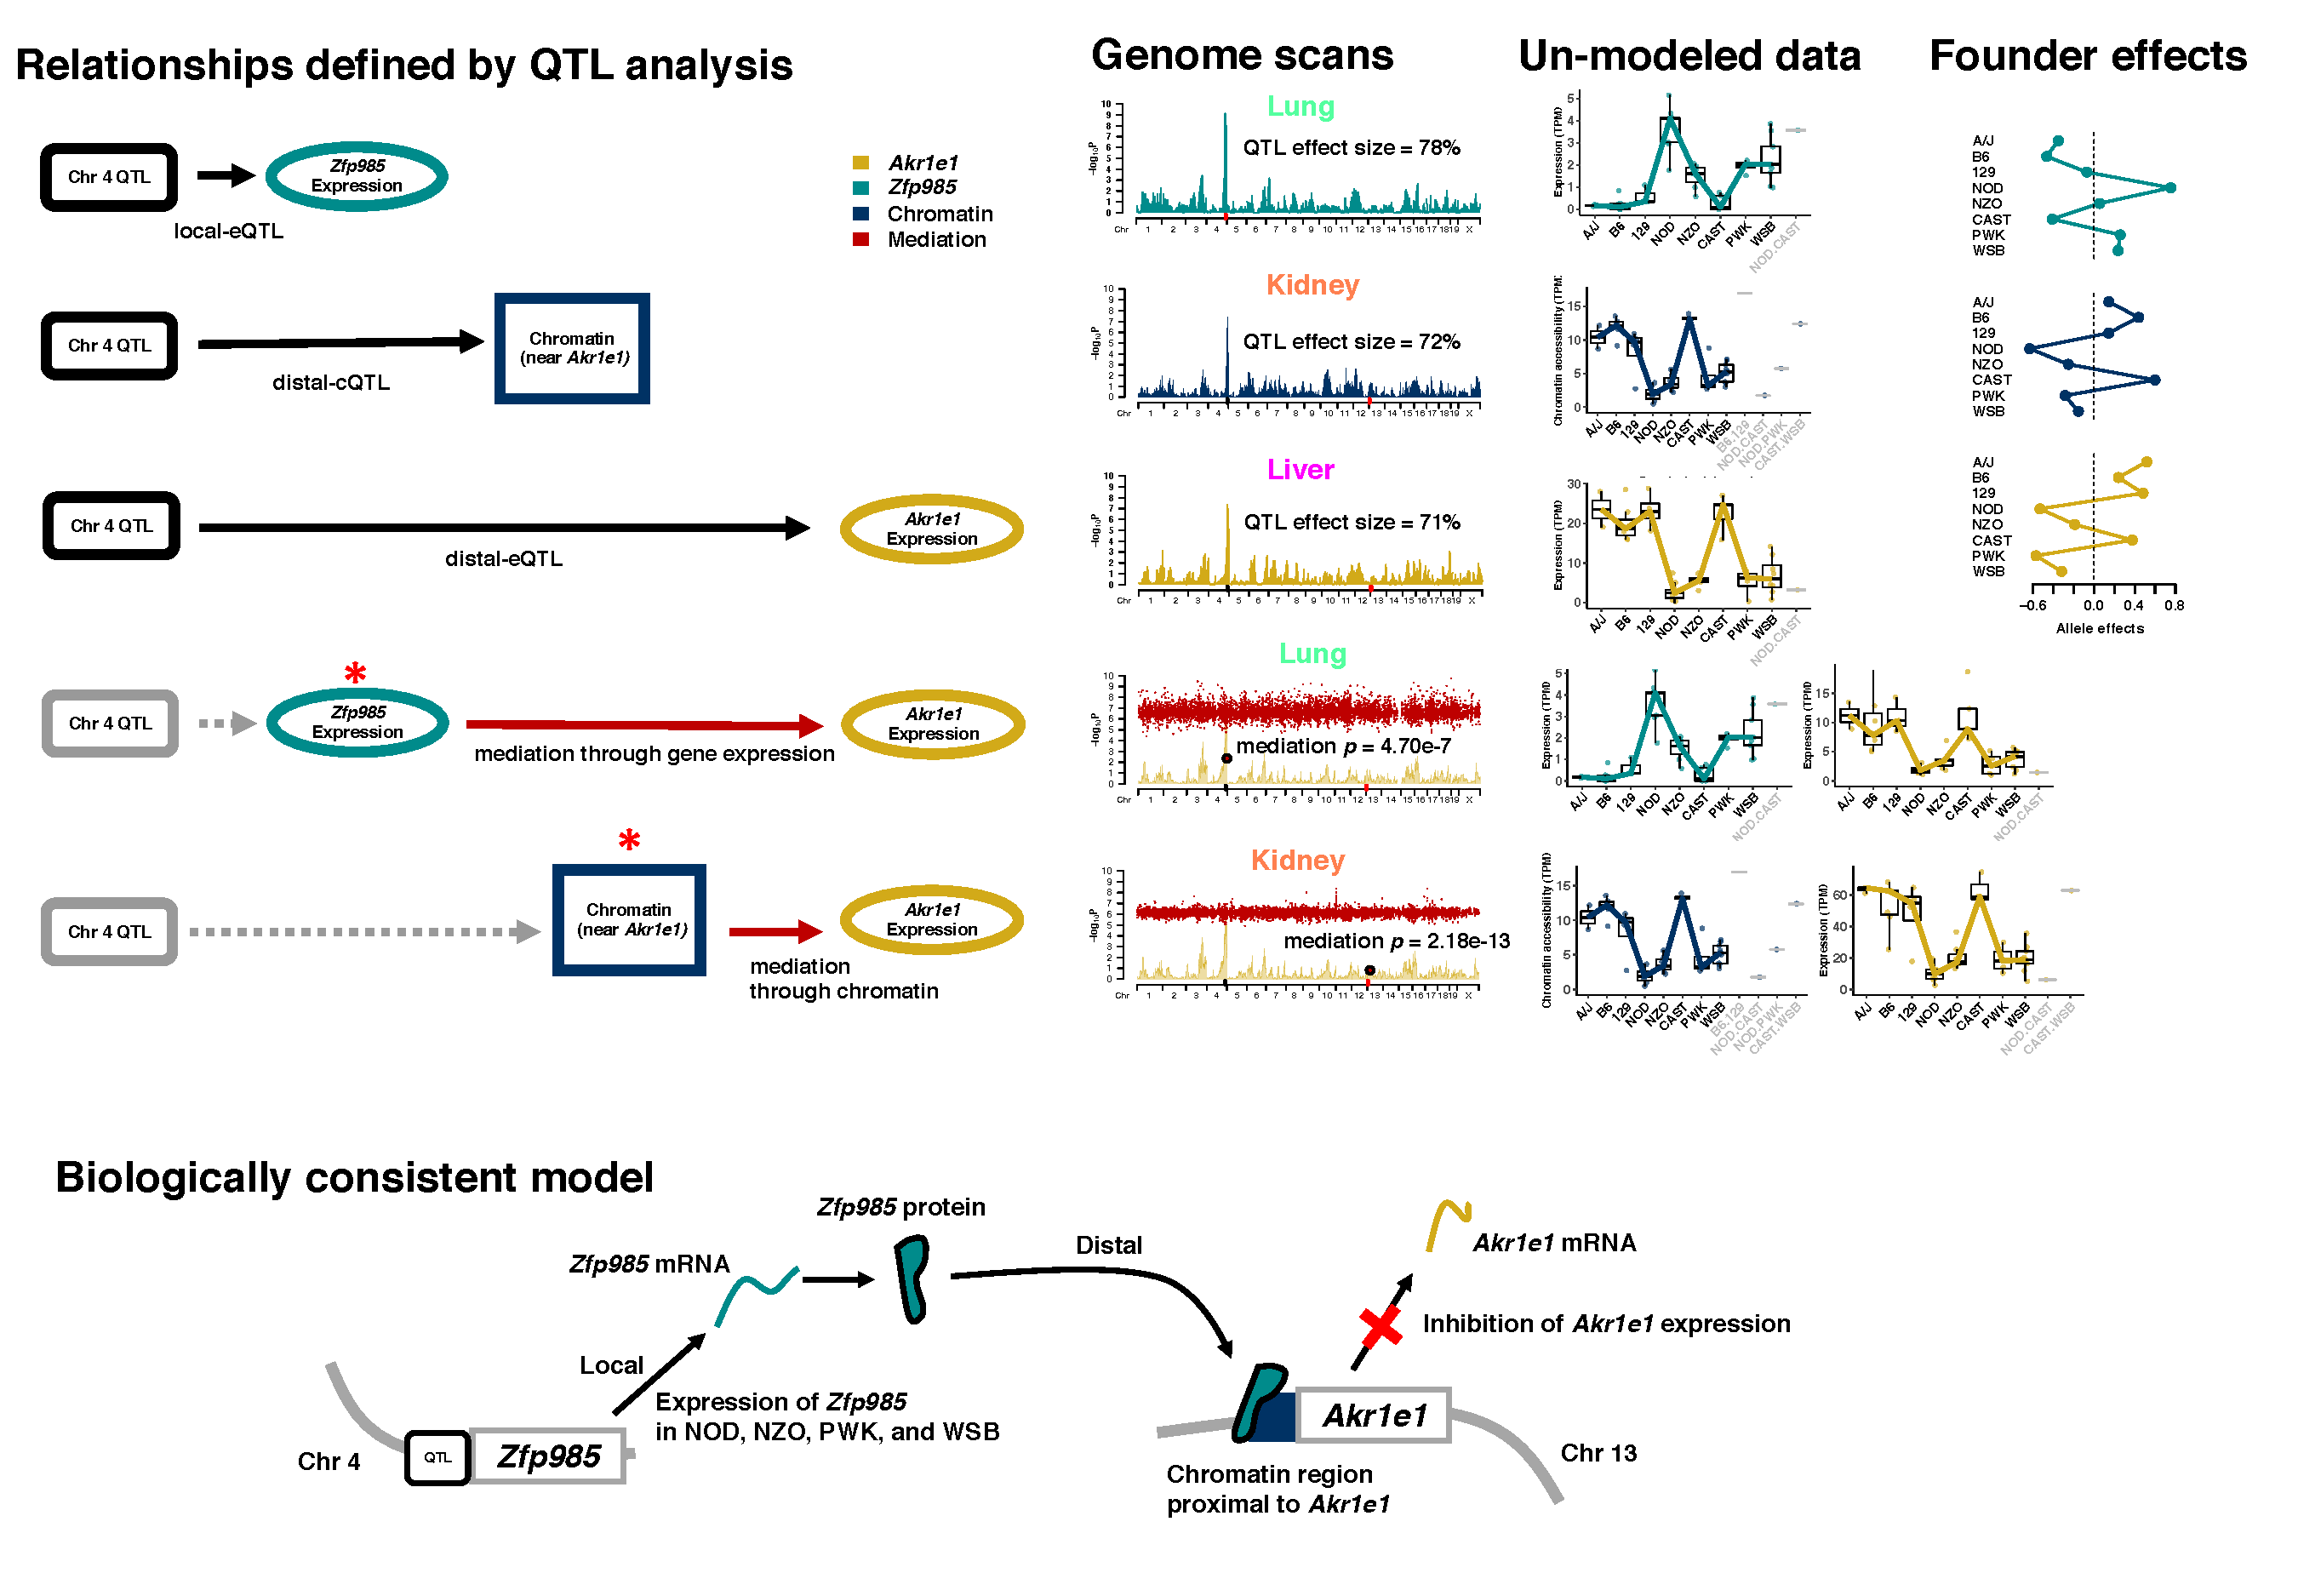
\includegraphics[width=\textwidth, trim={0in 0.1in 0in 0in}, clip]{figs/akr1e1_full_model_update.pdf}
\caption{\textbf{Complex mediation model for \textit{Akr1e1} distal-eQTL.}  The genetic regulation of \textit{Akr1e1} expression is reconstructed based on relationships observed across the three tissues. Distal-eQTL are detected in all tissues at similar levels of significance. A local-eQTL for \textit{Zfp985} that is proximal to the \textit{Akr1e1} distal-eQTL was observed in lung, and \textit{Zfp985} expression is detected as anti-correlated mediator of the distal-eQTL, consistent with \textit{Zfp985} suppressing \textit{Akr1e1} expression. The chromatin site proximal to the \textit{Akr1e1} TSS has a distal-cQTL detected in kidney. The chromatin accessibility at the site was found to be a significant correlated mediator of \textit{Akr1e1} expression. Combining associations across tissues supports a biological model whereby \textit{Zfp985}, expressed in mice with NOD, NZO, PWK, and WSB haplotypes, inhibits the proximal chromatin accessibility at the \textit{Akr1e1} TSS. QTL and mediation genome scans are included, along with sequence phenotypes as boxplots categorized according to most likely diplotype, and modeled founder effects fit as BLUPs. The relative magnitudes of the QTL effect sizes and mediation significance are consistent with the proposed model, with \textit{Zfp985} local-eQTL > chromatin distal-eQTL > \textit{Akr1e1} distal-eQTL and chromatin mediation > mediation through \textit{Zfp985} expression.
\label{fig:akr1e1_full_model}}
\end{figure*}

\subsubsection{\GKinline{Genetic regulation of \textit{Akr1e1} expression includes zinc finger protein and chromatin intermediates.}}
As detailed above, \textit{Akr1e1} possesses a strong distal-eQTL\WV{}{Akr1e1 not mentioned in the text before now that I could see.}\GK{}{In the paragraph on multi-tissue distal-eQTL (Figure 6A).}, observed in all three tissues with significantly correlated founder effects. Additionally, we found that this effect is strongly mediated through Zinc finger protein 985 (\textit{Zfp985}) expression in lung. The \textit{Zfp985} TSS is located on chromosome 4 at 147.6Mb, while the \textit{Akr1e1} distal-eQTL coordinates are 142.5Mb, 143.2Mb, and 148.6Mb in liver, lung, and kidney, respectively (\textbf{Figure \ref{fig:akr1e1_exmediation}}). \textit{Akr1e1} and \textit{Zfp985} expression are negatively correlated ($r = -0.69$), which is consistent with \textit{Zfp985} inhibiting \textit{Akr1e1} expression. This same distal-eQTL and mediator relationship for \textit{Akr1e1} was observed in kidney tissue from 193 DO mice (\textbf{Figure \ref{fig:do_akr1e1}}).

The presence of distal genetic regulation for \textit{Akr1e1} was previously described in \cite{HamiltonWilliams2013}. The distal-eQTL we detect are highly proximal to their \textit{Idd9.2} region \citep{HamiltonWilliams2010}, originally defined as spanning 145.5-148.57Mb of chromosome 4 and subsequently using NOD mice congenic with C57BL/10 (B10) introgressions \cite{HamiltonWilliams2013}. The B10 haplotype was found to be protective against the development of diabetes, characteristic of NOD mice. \textit{Akr1e1} is involved in glycogen metabolism and the larger \textit{Idd9} region harbors immune-related genes, implicating \textit{Akr1e1} and other genes located in and regulated by \textit{Idd9} as potential diabetes-related genes. 
Consistent with these studies, CC strains with NOD inheritance at the distal-eQTL have low expression of \textit{Akr1e1}. Genetic variation from B10 is not present in the CC, but the closely related B6 founder has high expression of \textit{Akr1e1} like B10. Similar to NOD, NZO, PWK, and WSB haplotypes result in low \textit{Akr1e1} expression, while A/J, 129, and CAST haplotypes join B6 as driving high expression (\textbf{Figure \ref{fig:akr1e1_full_model}}). Lowly expressed \textit{Zfp985} is a strong candidate for driving these effects on \textit{Akr1e1}.

Further elucidation of the genetic regulation of \textit{Akr1e1} was observed in kidney tissue, where a strong distal-cQTL is mapped to the \textit{Idd9.2} region for the chromatin site proximal to \textit{Akr1e1}. Based on the close proximities of the chromatin window to \textit{Akr1e1} and the distal-cQTL to the distal-eQTL, we mediated the distal-eQTL effect on the chromatin window, which was highly significant (permP = $\num{2.18e-13}$). The founder effects for the distal-cQTL are correlated with the distal-eQTL effects correlated ($r = 0.92$). The relative magnitudes of the QTL effect sizes and mediation $p$-values, shown in \textbf{Figure \ref{fig:akr1e1_relationships}}, support a causal model whereby \textit{Zfp985} expression reduces the expression of \textit{Akr1e1} by altering chromatin accessibility in the \textit{Akr1e1} promoter region (\textbf{Figure \ref{fig:akr1e1_full_model}}). 

%%%%%%%%%% Discussion
\section{Discussion}

We performed QTL mapping on gene expression and chromatin accessibility data in 47 CC strains. We have described the use of multiple procedures of varying statistical stringency to allow for detection of lower effect local-QTL, important in a study with a restricted sample size. 
Furthermore, we described statistical approaches for two models of the mediation of the eQTL effects, one through chromatin accessibility for local-eQTL, and the other through activity of proximal genes as measured through their expression for distal-eQTL. We oriented our mediation through chromatin accessibility on local-eQTL, for which this study is better powered, and find significant support that mediation through chromatin is present (4.2-9.6\% of local-eQTL across the tissues). Certain regions of the genome could not be assessed for cQTL or chromatin mediation due to ATAC-seq read alignment ambiguity, further restricting our ability to assess mediation. Despite these constraints, our results are consistent with the role of accessible chromatin regions in the regulation of gene expression \citep{Klemm2019}. Despite being underpowered to detect gene expression mediators of distal-eQTL we do find a number of strong candidates, including zinc finger protein genes.
%\WV{}{Inert paragraph somewhere (maybe near the back) discussing this study in relation to \citet{Keele2019} and what this study says about power for detecting eQTL, cQTL, mediation, etc. Could use to reiterate justification of three mapping procedures.}

\subsection{\GKinline{Expectations for QTL mapping power}}

\GKinline{QTL mapping power in a mature set of strains was recently evaluated through simulation \citep{Keele2019}. Given a sample of 47 strains, this study has approximately 80\% to detect QTL with a 55\% effect size at genome-wide significance. The effect size estimates, shown as red dots in \textbf{Figure \ref{fig:qtl_effect_sizes_by_method}}, are consistent with this expectation and potentially inflated due to the Beavis effect \citep{Xu2003}. These constraints in the sample size stress the importance in leveraging additional information, primarily the prior support for local genetic regulation, to detect more QTL when appropriate, which motivated our use of multiple analyses with different scopes, either genome-wide or local chromosome-wide.}

%\subsection{Multiple procedures for QTL detection}
%
%\WV{The use of multiple procedures for QTL detection allowed us to assess varying degrees of statistical support for their associations, and of particular importance, leverage prior belief in the predominance of local associations in order to detect higher numbers of QTL for a sample of 47 mice. The multi-stage procedure (Method 1) allowed for genome-wide detection of multiple QTL per outcome while incorporating both FWER and FDR adjustments. Both the chromosome-wide FDR (Method 2) and local-only (Method 3) analyses strongly increase power to detect local-QTL, but lose the ability to identify distal-QTL located on other chromosomes.
%}{Move to methods/results. That is where this justification is sorely needed. Make more of the prior belief stuff.}
% \subsection{Distal-QTL on local chromosome}

% We find that we are powered to detect distal-QTL predominately located on the local chromosome, as seen in \textbf{Figure \ref{fig:grid_plot}}. Many FWER-significant (permP < 0.05) distal-QTL on non-local chromosomes are filtered by the FDR procedure, such as the distal-eQTL for \textit{Ccnyl1}, shown in \textbf{Figure \ref{fig:exmediation}}. The mediation of this distal-eQTL through zinc finger proteins strongly suggests that it is a real distal-eQTL. It is possible that distal-QTL on non-local chromosomes tend to be of lower effect than distal-QTL located on the local chromosome, though far from the gene or chromatin site, and these data are not sufficiently powered to detect non-local chromosome distal-QTL. 

\subsection{Joint QTL analysis in multiple tissues}

Recent research, such as the GTEx project \citep{GTEX2017}, comprised of expression data from 44 human tissues, reflects a growing interest in interrogating and characterizing differences in gene expression and its regulation across a wide range of tissues. Previous studies in mice (\eg \citealt{Huang2009}) have used tissue-specific or stratified QTL analyses, similar to as done here, and then characterized the overlap across tissues. Our use of formal statistical tests of the correlation coefficient between the founder haplotype effects of overlapping QTL is, to our knowledge, \GKinline{a novel approach to formally defining overlapping QTL, allowing for the identification of QTL with unique founder effects patterns, likely representing distinct tissue-specific QTL. This was observed with three local-eQTL for the gene \textit{Pik3c2g} (\textbf{Figure \ref{fig:pik3c2g}}), and potentially represent tissue-specific local regulation.}

\GKinline{This approach can also identify consistent haplotype effects, as with the gene \textit{Per2} (\textbf{Figure \ref{fig:correlated_distal_eqtl}B}), which possessed marginally significant intra-chromosomal distal-eQTL observed across the three tissues, which also suggests that it would be more powerful to map QTL in all tissues jointly.} Formal joint analysis approaches have been proposed, largely implemented for SNP association, including meta-analysis on summary statistics (\eg \citealt{Fu2012a, Sul2013}) and fully joint analysis, including Bayesian hierarchical models \citep{Flutre2013} and mixed models \citep{Acharya2016}. Extending such statistical frameworks to haplotype-based analysis in MPP, as used here, poses some challenges, including how to best generalize these approaches to the more complex genetic model, and in the context of the CC where the number of unique genomes is limited. Nevertheless, such approaches would certainly be more powerful and principled for detecting and calling QTL present across multiple tissues, and should be considered for future related research in the CC and similar populations, such as the DO. When multiple levels of molecular traits are measured on each individual, there is also the potential to incorporate joint analyses into the mediation framework, which could also presumably improve detection power.

\subsection{Correlated founder effects suggest multi-allelic QTL}

Haplotype-based association in MPP allows for the detection of multi-allelic QTL \citep{Aylor2011}, such as observed with the kidney local-eQTL of \textit{Pik3c2g} in which mice with B6 contributions in the region have an intermediate level of expression. The correlation coefficient between the founder haplotype effects for QTL pairs provides an interesting summary, generally not possible in the simpler bi-allelic setting commonly used in variant association. The extent of the correlation between the founder effects for QTL pairs of certain genes, such as \textit{Cox7c} and \textit{Ubc} (\textbf{Figure \ref{fig:correlated_local_eqtl}A}) suggests that these QTL are at least subtly multi-allelic. Correlated founder effects are consistent with genetic regulation, even local to the gene TSS, being potentially complex with strain-specific modifiers.

\subsection{Correlated founder effects in the presence of differential expression}

We detected numerous genes with QTL pairs with correlated founder effects across tissues despite the overall expression patterns being significantly different based on the differential analysis; examples include \textit{Cox7c}, \textit{Ubc}, \textit{Slc44a3}, and \textit{Akr1e1}. We propose two primary explanations for the unique co-occurence of consistent genetic regulation of genes with expression profiles that vary significantly across tissues. 

First, the samples used in the study represent bulk tissue samples, and thus possess cellular heterogeneity that likely varies between liver, lung, and kidney tissues. DE signal may simply represent the varying cellular compositions of the tissues. Single cell sequence experiments would reduce noise from tissue heterogeneity, though the results would no longer reflect averages across the overall tissue. Statistical approaches that aim to estimate the cellular composition of a tissue \citep{Aran2017} have been developed, which could provide some insights into how the tissues vary from each other. 

Second, and alternatively, DE genes that share QTL across tissues could be real, and suggest that other tissue-specific modifiers of expression are active that alter the magnitude of the expression profile. Single cell sequencing experiments could be used to confirm such patterns in the genetic regulation of expression.

\subsection{Mediation analysis}

Our approach to mediation analysis is related to previous studies in DO mice \citep{Chick2016,Keller2018,Skelly2019}, though with modification, including the use of QTL effect sizes to establish consistency with the directionality of the mediator relationship and the formal calculation of a mediation $p$-value through permutation (permP).  To our knowledge, such mediation analyses have not been used in the CC, though related conditional regression approaches were used in the incipient CC lines \citep{Rutledge2014, Kelada2014}. Mediation within the field of system genetics is a growing area of interest.
%, and the methods proposed here support that development.

Determining causality, particularly in a biological system as complex as transcriptional regulation in bulk tissue samples, is impossible. These mediation analyses will largely reflect the correlations between the variables after adjusting for additional sources of variation, such as covariates and batch effects. Our additional step of requiring the mediator QTL to have a larger effect size than outcome QTL aims to identify trios that are consistent with the proposed mediation models. It is possible that the measurement of the mediator is a noisier process compared to the measurement of the outcome, which would result in the effect size of the mediator QTL being reduced, and thus potentially a false negative mediation result. Complex relationships with many factors or levels of feedback are also unlikely to be detected.

Despite these limitations, mediation analysis can provide specific candidates underlying detected QTL, particularly in comparison to considering all genes near the QTL peak. The genetic regulation of \textit{Akr1e1} (\textbf{Figure \ref{fig:akr1e1_full_model}}) provides a strong example case in which a single gene, \textit{Zfp985}, in the eQTL region is identified as a strong mediator. It is possible that \textit{Zfp985} is not the true mediator, but is instead strongly correlated with it. For comparison, \cite{HamiltonWilliams2013} proposed \textit{Rex2} as a candidate, which was filtered out for having low expression from all three tissues in this study, whereas \textit{Zfp985} was lowly expressed but successfully quantified in lung. Disentangling the relationships underlying QTL poses a strong challenge, and mediation analyses can provide strong candidates for downstream experiments for validation. Additionally, mediation analysis provides strong support that the causal mediator inhibits \textit{Akr1e1} expression by reducing chromatin accessibility near its TSS.

\subsection{\GKinline{Reliability of QTL effect size estimates}}

%\WV{}{This subsection comes across largely as arcane CC-specific inside baseball. Placing it here risks announcing that this is our most interesting finding. Also, the removal of the ranef effect size method makes it moot. If anything, you could write something else about the Beavis effect, seeing as it should be relevant.}

Estimation of the variance explained by the QTL, here referred to as the effect size, can provide an interpretable point summary for haplotype-based QTL mapping, analogous to the effect of the minor allele, commonly used in SNP association. We recorded two estimates of effect size, one based on a fixed effect fitting of the QTL term whereas the other included the QTL as a random term \citep{Wei2016}. 
%Both estimates of effect size possessed unique and appealing qualities. 
\GKinline{We primarily report results from the fixed effects estimate because these were largely consistent with the expectations found by \cite{Keele2019} for a study of this size, whereas the conservative shrinkage-based estimate were overly reduced. The mapping results are largely consistent with the genetic regulation of these molecular traits being largely Mendelian, with large effect sizes (> 60 \%).}
%, though more complex genetic regulation is suggested by QTL with smaller effect sizes (< 50\%) when detecting local-QTL with reduced stringency.
\GKinline{The shrunken effect size estimates can potentially identify putative QTL with unstable fixed effect estimates due to influential data points. Notably, a small number of the distal-eQTL have very low random effect size estimates (\textbf{Figure \ref{fig:qtl_effect_size_fixefvsranef}}) compared to their fixed effects-based estimates.}
%Notably, QTL with this pattern of effect size estimates are largely distal. A mapping procedure that fits the QTL effect as a random effect, as in \cite{Wei2016}, would likely not detect these QTL. However, a random effects procedure is more computationally intensive, which is particularly unappealing in the context of genome-wide molecular traits, thus justifying a follow-up approach in which effect sizes are evaluated for the detected QTL.

\subsection{Conclusion}

In summary, in this study we have performed QTL and mediation analyses of gene expression and chromatin accessibility data in liver, lung, and kidney tissue samples from 47 strains of the CC. We use the formal statistical testing of correlation coefficient between founder haplotype effects of overlapping QTL to identify QTL that are likely functionally active in multiple tissues as well as likely distinct tissue-specific QTL, as is the case with the gene \textit{Pik3c2g}. We detect extensive evidence of chromatin mediation of local-eQTL as well as gene expression mediators underlying distal-eQTL. One unique example is the elucidation of the genetic regulation of \textit{Akr1e1} expression, a gene that plays a role in glycogen metabolism, involving distal inhibition by a zinc finger protein mediator that reduces chromatin accessibility at the TSS. These findings highlight the ability of integrative QTL approaches, including mediation analysis, to identify interesting biological findings, including the ability to identify functional candidates for further downstream analysis.

\section{Acknowledgments}
This work was funded by grants from the National Institute of Environmental Health Sciences (NIEHS) (R01-ES023195 to IR and GEC and P30-ES025128), with GRK and WV funded by grants from the National Institute of General Medical Sciences (NIGMS) (R01-GM104125 and R35-GM127000 to WV). We are grateful for discussions with Gary A.\ Churchill on mediation analysis that influenced this work. Additionally GRK was partially supported through funding from Dr.\ Churchill and The Jackson Laboratory.

Author contributions: GRK, BCQ, WV, and TSF wrote the manuscript. GRK, BCQ, and WV developed the statistical methods for QTL analysis, and GRK wrote the software to perform the respective analyses. BCQ processed the sequence data and performed the DE and DAR analyses. GRK and BCQ performed all QTL and mediation analyses. The authors declare no conflicts of interest.

\bibliography{eQTL_mediation.bib}

\clearpage

%%%%%%%%%% Appendices
\section{\GKinline{Appendix A: CC strains}}

\GKinline{This study included males from the following 47 CC strains: CC001, CC002, CC003, CC004, CC005, CC006, CC007, CC010, CC011, CC012, CC013, CC015, CC016, CC017, CC019, CC020, CC021, CC023, CC024, CC025, CC027, CC028, CC029, CC030, CC031, CC032, CC033, CC035, CC036, CC037, CC038, CC039, CC040, CC041, CC042, CC043, CC044, CC045, CC046, CC049, CC053, CC055, CC057, CC059, CC061, CC062, and CC068.}

\section{\GKinline{Appendix B: False positive control}}

%\WV{}{This appendix material should be heavily thinned, potentially put into the Methods}

\GKinline{QTL detection in the context of genome-wide scans across a large number of traits needs to account for a heavy multiple testing burden. This can be done in a two-step approach.}
%In order to efficiently detect QTL, we used three procedures to define statistical significance over varying stringency, allowing greater leniency for putative local genetic regulators. These procedures address the family-wise error rate (FWER) and false discovery rate (FDR) differently.

\subsection{\GKinline{Family-wise error rate}}

\GKinline{For a given trait, we seek to control the family-wise error rate (FWER), the probability of a single false positive being detected across all tests. FWER can be controlled through adjustment of the observed maximum logP based on an extreme value distribution (EVD) defined from permutation scans, ultimately producing an FWER-adjusted $p$-value (permP). This adjustment can be done at either genome-wide or the more lenient local chromosome-wide significance. Analysis L used only these FEWR-controlling thresholds for QTL detection, ignoring the multiple testing burden that results from testing many traits and instead relying on a strong prior belief in local genetic regulation.}

\subsection{\GKinline{False discovery rate}}

%\GKinline{With eQTL and cQTL analysis, many genome scans are being performed for each molecular trait, representing an additional source of multiple testing. However, in contrast to the expectation of relatively few QTL affecting a single trait, we expect many of these traits to possess QTL, thus motivating a more lenient control of false positives. To account for multiple testing over many traits, a false discovery rate (FDR) adjustment \citep{Benjamini1995} can be used to produce $q$-values, which are interpretable as the probability that a detected QTL is a false discovery.} 

%The family-wide error rate (FWER) is the probability of detecting a single false positive across all genome-wide tests. Controlling FWER instead of the single test type I error rate ($\alpha$) is necessary because FWER increases with the number independent tests, reaching 1 for $\alpha = 0.05$ in the context of genome-wide tests. Controlling FWER is more conservative than controlling the false discovery rate (FDR) for multiple testing correction, and appropriate for genome scans of a single trait because there are not expected to be an excess number of QTL per outcome. 

%Based on simulations of the breeding design \citep{Valdar2006c}, the CC panel was expected to be balanced in terms of founder haplotype contributions. This balance was realized to large extent \citep{Srivastava2017}, though the PWK and CAST founders have reduced contributions in comparison to the other founders. \cite{Keele2019} performed simulations from the realized CC strain genomes to examine QTL mapping power, and found low levels of population structure in the CC genomes, violating the exchangeability assumption made by the permutation procedure, which characterizes a null distribution for the test statistic\citep{Doerge1996}. Nevertheless, we use a permutation approach, given that we expect the presence of strong effect QTL for the molecular traits that are detectable in the presence of subtle population structure.

%Specifically, 1000 permutations of the sample identities were taken, and then genome scans performed on each permutation of each trait. For each trait, the minimum p-value from each permutation genome scan is recorded, transformed to the -$\log_{10}$ scale (logP), and then used fit a null extreme value distribution (EVD) \citep{Dudbridge2004,Valdar2006c}. Genome-wide permutation-based p-values (permP) are obtained by calculating the probability of a more extreme logP than the observed from the cumulative distribution function of the EVD.

\GKinline{Analyzing a large numbers of traits, as is the case with gene transcripts or chromatin accessibility sites, also contributes significantly towards the multiple testing burden: not only is an association for a trait being tested at positions across the genome, but the whole process is repeated for each trait. The expected number of significant tests differs globally across all the traits, with many traits expected to have QTL in comparison with few QTL being expected for a single trait.}

\GKinline{An FDR procedure can address this multiple testing dynamic, accounting for the additional testing due to many traits while being more lenient than strict FWER control across traits. An FDR procedure \citep{Benjamini1995,Storey2003} was applied to the per-trait permP, producing $q$-values. QTL are detected if q-value $\le \alpha_{\text{FDR}}$, where $\alpha_{\text{FDR}}$ is the specified false discovery rate. QTL were called using both $\alpha_{\text{FDR}} = 0.1$ and $\alpha_{\text{FDR}} = 0.2$. Analysis LC used permP derived EVD defined from the local chromosome, and Analysis G used genome-wide permP.}

%\section{Appendix C: Mapping procedures}

\section{\GKinline{Appendix C: Conditional genome scans (Analysis G)}}

The combined per-trait FWER control and across-trait FDR control restrict the mapping procedures ability to detect multiple QTL per outcome in a statistically valid manner because the EVD used for FWER adjustment is fit from the maximum statistical score per trait. To include additional strong statistical scores is potentially biasing, as would be the case when there are multiple associations above the FWER threshold, increasing the enrichment in small $p$-values. This inflation is precisely the pattern of association the FDR procedure detects. To avoid this problem, a multi-stage conditional fitting approach is used \citep{Jansen2017}. The procedure is described in the following steps:
\begin{enumerate}
	\item For a given trait, conduct genome scan according to the model described in Eq \ref{eq:alternative_model}.
    \item Perform genome scans for the permuted trait to characterize an EVD. Calculate FWER-adjusted permP from the observed maximum logP of the genome scan of the trait. The permP is stored to be used as input to an FDR method.
    \item Specify a genome-wide $\alpha_{\text{step}}$ for determining whether subsequent conditional scans should be conducted for the trait. We set $\alpha_{\text{step}} = 0.1$. If the $\text{permP} > \alpha_{\text{step}}$, no further conditional scans are conducted.
    \item If $\text{permP} \le \alpha_{\text{step}}$, steps 1-3 are repeated for additional conditional scans of the outcome. For $j > 1$, $j^{\text{th}}$ conditional scan use the same form of alternative and null model as described in Eq \ref{eq:alternative_model}, except with the inclusion of locus effects from the peak associations from previous stages. Generally, the alternative model for conditional stage scan $J$ follows as:
\begin{equation}
y_{i} = \mu + \text{QTL}_{i} + \sum_{j=1}^{J-1}\text{locus}_{i}^{j} + \text{batch}_{i} + \varepsilon_{i},
\label{eq:conditional_model}
\end{equation}
with $\text{locus}_{i}^{j}$ representing the locus effect of the peak association from the $j^{\text{th}}$ stage scan of the outcome for individual $i$, and is also included in the null model of conditional scans. Now steps 2-4 are repeated.
\end{enumerate}

A multi-stage conditional scan approach could have issues with over-fitting 47 data points per trait, given that each $\text{QTL}$ and $\text{locus}$ effect represents the estimation of seven fixed effects. However, the permutations were found to appropriately compensate for this potential in the recalculation of the EVD based on permutations of the conditional scans in step 2. \textbf{Figure \ref{fig:conditional_scans}} provides a clear example in which the gene \textit{Gpn3} has a local-eQTL detected after a strong distal-eQTL is conditioned for within the model in lung tissue. This multi-stage conditional procedure is referred to as Analysis G.

%\subsection{Method 2: Single-stage regression with chromosome-wide FWER and FDR control}

%Given that the data represent 47 individual mice, there may be poor power to detect genome-wide significant QTL. Because of the strong biological prior evidence for local-QTL, significant genetic associations that meet chromosome-wide significance for the local chromosome of the trait were also detected and recorded. This was accomplished by fitting a chromosome-wide EVD, and thus producing chromosome-wide FWER-adjusted permP for each trait. Chromosome-wide results were restricted to the first stage of the multi-stage procedure, thus referred to as a single-stage analysis, and allowing only a single chromosome-wide permP per trait. The same FDR then used as in Method 1, resulting in chromosome-wide q-values. This more lenient single-stage procedure is referred to as Method 2.

%\subsection{Method 3: Single-stage regression with genome-wide and chromosome-wide FWER control for local-QTL}

%A final local-QTL exclusive single step analysis is used. Instead of calculating genome-wide and chromosome-wide permP from the overall maximum logP, FWER-controlled permP are adjusted from the maximum logP within the proximal window of the trait from the first stage scans from Method 1. An FDR procedure is not used, in part because the permP are likely to be poorly distributed with respect to the expectations of FDR. A local-QTL is detected when $\text{permP} < 0.05$. This procedure, now referred to as Method 3, is less conservative for local-QTL because there is no FDR control, instead leveraging the strong biological precedent for proximal genetic regulation. It also does not leniently detect intra-chromosomal distal-QTL, as with Method 2.

\section{Appendix D: Mediation analysis}

\cite{Baron1986} give a description of the relationships that need be tested to declare mediation. For this study, simple models that consist of three variables are used: the independent variable X, the mediator M, and the dependent variable Y \citep{MacKinnon2007}. Superscripts are used to indicate whether a variable is the QTL, chromatin accessibility at site $k$ ($\text{C}_{k}$), or expression of gene $j$ ($\text{G}_{j}$) in the model. When an eQTL is detected, the following relationship is supported:
\begin{equation}
\text{X}\textsuperscript{QTL} \quad \rightarrow \quad \text{Y}^{\text{G}_{j}}
\label{rel:eQTL}
\end{equation}
When cQTL or proximal eQTL to distal-eQTL are detected, a similar relationship is detected:
\begin{equation}
\text{X}\textsuperscript{QTL} \quad \rightarrow \quad \text{M}
\label{rel:cQTL}
\end{equation}
The previous traits (Y) can also be viewed as potential mediators (M). Here we consider two models of mediation: 1) the effect of an eQTL is mediated through local chromatin state ($\text{M}^{C_{k}}$) and 2) the effect of the distal-eQTL is mediated through a proximal gene ($\text{M}^{G_{k}}$), depicted in \textbf{Figure \ref{fig:graph}}. Co-localizing QTL are consistent with the co-occurrence of $X \rightarrow Y^{G_{j}}$ and $X \rightarrow Y^{C_{k}}$ at a locus. A true mediation relationship has an additional requirement, specifically that: 
\begin{equation}
\text{X}\textsuperscript{QTL} \quad \indep \quad \text{Y}^{\text{G}_{j}} \quad | \quad \text{M}
\label{rel:full_mediator}
\end{equation}
where ``A $\indep$ B'' indicates that A and B are independent of each other, and ``A|B'' is A conditioned on variable B. X being fully independent of Y given M is consistent with X acting on Y completely through M, referred to as full mediation. In practice, the true relationship can be complex and obscured by noise, instead resulting in partial mediation, whereby X affects Y both directly and through M. Genome-wide data present a significant challenge to systematically testing these relationships.

\subsection{Mediation models}

\subsubsection{Mediation of local-eQTL through chromatin state.}
Mediation through chromatin accessibility was evaluated for all local-eQTL detected through the lenient Analysis L, leveraging prior knowledge of the predominance of local genetic regulation and the effects of proximal chromatin state. Candidate mediators are detected at genome and chromosome-wide significance through 1,000 permutations to define EVD for FWER adjustment.

\subsubsection{Mediation of distal-eQTL through proximal gene expression.}
Mediation of the effect of genome-wide significant distal-eQTL through proximal gene expression was evaluated. Genome-wide significance is required for distal-eQTL because there is not additional strong biological information to support increased leniency as is the case with proximal signal. As with mediation through chromatin state, 1,000 permutations are used to define mediation significance thresholds at the genome-wide level. 

Mediation of cQTL through other chromatin sites and gene expression were also evaluated, but did not result in the detection of any candidate mediators.

\subsection{Mediation significance thresholds}

Empirical significance thresholds for the mediation scans can be defined through permutations, similarly to as is done with the QTL scans. Instead of permuting the trait outcome, the pairing of trait to QTL is maintained, and the mediator is permuted. EVD are then fit for potential mediators from the minimum logP from permutation scans, instead of the maximum logP in QTL scans. FWER-adjusted mediation permP are extracted from the EVD, which can be calculated in terms of genome-wide and chromosome-wide significance. An FDR adjustment is not used with mediation because it is only evaluated for detected QTL, which could potentially violate the uniform null distribution expectations of FDR.

\subsection{Formal mediation criterion}

Detection of mediation has some caveats and pitfalls compared to the statistical analyses used for QTL mapping, in part due to the fact that the relationships \ref{rel:eQTL} and \ref{rel:cQTL} could be complex, whereas the directionality of the relationships for QTL is fixed because the genetic state at the QTL cannot change due because of the trait. This does not hold for the mediation model, where Y could in fact causally influence M (Y $\rightarrow$ M). \cite{Didelez2007} note that false mediation signals can be detected when the association between the M and Y are particularly strong, whereby M acts as a surrogate for X. Based on concerns over fitting relatively complex models to data comprising 47 observations, we use stringent requirements for declaring evidence for mediation:
\begin{enumerate}
	\item Detection of a significant eQTL (relationship \ref{rel:eQTL}).
    \begin{enumerate}
    	\item Mediation through chromatin: chromosome-wide permP < 0.05 from Analysis L
        \item Mediation through expression: genome-wide q-value < 0.1 from Analysis G
    \end{enumerate}
    \item Detection of significant mediator within a 20Mb window centered around the eQTL from previous step.
    \item Detection of a significant QTL for the mediator from previous step.
    \begin{enumerate}
    	\item Mediation through chromatin: chromosome-wide permP < 0.05 from Analysis L and within 10Mb upstream or downstream of gene TSS
        \item Mediation through expression: genome-wide q-value < 0.1 from Analysis G and within 10Mb upstream or downstream of the eQTL position
    \end{enumerate}
    \item It is not possible to distinguish M $\rightarrow$ Y from M $\leftarrow$ Y given these data. If M is an intermediary of X on Y, the expectation is that the effect of X $\rightarrow$ M is greater than X $\rightarrow$ Y. We check that the effect size of the QTL for step 1 (X $\rightarrow$ Y) is less than the effect size of the QTL from step 3 (X $\rightarrow$ M). Failure of this step does not disprove the proposed mediation model, but it could suggest that the relationship between M and Y is more complicated than the simple models tested here, or that greater noise is incurred in the measurement of M than Y.
\end{enumerate}

\clearpage

%%%%%%%%%% Description of supplement
\section{Data and Supplement details}

Data and analysis files in the \textbf{Supplement} include:

\begin{itemize}
	\item File\_S1: data\_supplement\_details.pdf
	\item File\_S2: miqtl\_1.1.1.tar.gz
	\item File\_S3: cc\_genome\_cache.zip
	\item File\_S4 - S6: \{liver,lung,kidney\}\_expression.csv
	\item File\_S7 - S9: \{liver,lung,kidney\}\_chromatin.csv
	\item File\_S10 - S12: de\_\{liver\_lung,liver\_kidney,lung\_kidney\}.csv
	\item File\_S13 - S15: dar\_\{liver\_lung,liver\_kidney,lung\_kidney\}.csv
	\item File\_S16 - S18: \{liver,lung,kidney\}\_local\_eqtl.csv
	\item File\_S19 - S21: \{liver,lung,kidney\}\_distal\_eqtl.csv
	\item File\_S22 - S24: \{liver,lung,kidney\}\_local\_cqtl.csv
	\item File\_S25 - S27: \{liver,lung,kidney\}\_distal\_cqtl.csv
	\item File\_S28 - S30: \{liver,lung,kidney\}\_chromatin\_mediation.csv
	\item File\_S31: supplement\_tables\_figures.pdf
\end{itemize}

\section{miQTL package}

The static version of the miQTL R package (1.1.1) used for this work is provided in the \textbf{Supplement} as File\_S2. The current version of miQTL is available here: \url{https://github.com/gkeele/miqtl}. miQTL can be installed using the command `R CMD INSTALL' at the terminal. The current version from GitHub can be conveniently installed using the devtools R package and the following command within R: `install\_github(``gkeele/miqtl'')'.

\section{QTL and mediation analyses}

\section{File types}

\begin{itemize}
	\item *.R - These are R scripts used to run the statistical analyses and generate the figures.
	\item *.RData - The zipped directory contained in File\_S3 is composed of *.RData files that are HAPPY formatted, which miQTL is designed to use.
	\item *.csv - Comma-separated value files representing the trait data used for differential and QTL analyses and their large results tables, which were too large to be included as formatted tables.
\end{itemize}

\thispagestyle{empty}
\clearpage

%%%%%%%%%% Supplement
\section{Supplemental Tables and Figures}
\setcounter{table}{0}
\setcounter{figure}{0}
\renewcommand{\thetable}{S\arabic{table}}
\renewcommand{\thefigure}{S\arabic{figure}}
\setcounter{page}{1}

\begin{table*}[h]
\renewcommand{\familydefault}{\sfdefault}\normalfont
\begin{tableminipage}{\textwidth}
\captionsetup{width=\textwidth}
\centering
\caption{\bf Number of differentially expressed genes and accessible chromatin regions detected between liver, lung, and kidney tissues
\label{tab:diff_gene}}
\end{tableminipage}
\begin{tableminipage}{\textwidth}
\begin{tabularx}{\textwidth}{cll|XXX}
\hline 
& & & & \center{Tissue comparison} & \\
& & & Liver vs Lung & Liver vs Kidney & Lung vs Kidney \\
\hline
%%%%%%%%%%%%%%%%
\parbox[t]{5mm}{\multirow{6}{*}{\rotatebox[origin=c]{90}{q-value < 0.1}}} & 
Genes & Up-regulated & 2,473 (20.8\footnote{Percentage of all tested genes.\label{fn:total_perc_gene}}) & 2,123 (17.9\footref{fn:total_perc_gene}) & 2,246 (18.9\footref{fn:total_perc_gene}) \\
& & Down-regulated & 3,236 (27.2\footref{fn:total_perc_gene}) & 1,441 (12.1\footref{fn:total_perc_gene}) & 2,527 (21.3\footref{fn:total_perc_gene}) \\
& & Total & 5,709 (48.0\footref{fn:total_perc_gene}) & 3,564 (30.0\footref{fn:total_perc_gene}) & 4,773 (40.2\footref{fn:total_perc_gene}) \\
\cline{2-6}
& Chromatin Regions & Increased accessibility & 20,194 (19.6\footnote{Percentage of all tested chromatin regions prior to merging adjacent genomic windows.\label{fn:total_perc_chrom}}) & 15,252 (12.9\footref{fn:total_perc_chrom}) & 19,202 (17.4\footref{fn:total_perc_chrom}) \\
& & Decreased accessibility & 20,603 (19.7\footref{fn:total_perc_chrom}) & 12,796 (11.4\footref{fn:total_perc_chrom}) & 12,967 (11.2\footref{fn:total_perc_chrom}) \\
& & Total & 40,797 (39.3\footref{fn:total_perc_chrom}) & 28,048 (24.3\footref{fn:total_perc_chrom}) & 32,169 (28.6\footref{fn:total_perc_chrom}) \\
\hline
\end{tabularx}
\end{tableminipage}
\end{table*}

\begin{table*}[h]
\renewcommand{\familydefault}{\sfdefault}\normalfont
\begin{tableminipage}{\textwidth}
\captionsetup{width=\textwidth}
\centering
\caption{\bf Number of genes with eQTL detected in liver, lung, and kidney tissues
\label{tab:eqtl_mapping}}
\end{tableminipage}
\begin{tableminipage}{\textwidth}
\begin{tabularx}{\textwidth}{ll|XXX}
\hline 
& & & \center{Tissue (\%)} & \\
Procedure & eQTL type & Liver & Lung & Kidney \\
\hline
%%%%%%%%%%%%%%%%
Analysis G\footnote{Multi-stage conditional regression analysis with genome-wide FDR < 0.1. \label{fn:method_one}} & All & 520 (6.2\footnote{Percentage of all tested genes.\label{fn:total_perc}}) & 478 (4.2\footref{fn:total_perc}) & 739 (7.3\footref{fn:total_perc}) \\
& Local\footnote{10Mb upstream or downstream of gene TSS. \label{fn:local_eqtl}} & 400 (76.9\footnote{Percentage of genes with genome-wide eQTL.\label{fn:gw_eqtl_perc}}) & 369 (77.2\footref{fn:gw_eqtl_perc}) & 601 (81.3\footref{fn:gw_eqtl_perc}) \\
& Distal\footnote{More than 10Mb upstream or downstream of gene TSS or on another chromosome. \label{fn:distal_eqtl}} & 132 (25.4\footref{fn:gw_eqtl_perc}) & 112 (23.4\footref{fn:gw_eqtl_perc}) & 148 (20.0\footref{fn:gw_eqtl_perc}) \\
\hline
% %%%%%%%%%%%%%%%%
Analysis LC\footnote{Single-step regression analysis with chromosome-wide FDR < 0.1. \label{fn:method_two}} & All & 2,587 (30.8\footref{fn:total_perc}) & 2,069 (18.2\footref{fn:total_perc}) & 3,191 (31.6\footref{fn:total_perc}) \\
& Local\footref{fn:local_eqtl} & 1,749 (67.6\footnote{Percentage of genes with chromosome-wide eQTL.\label{fn:cw_eqtl_perc}}) & 1,498 (72.4\footref{fn:cw_eqtl_perc}) & 2,214 (69.4\footref{fn:cw_eqtl_perc}) \\
& Distal\footref{fn:distal_eqtl} & 838 (32.4\footref{fn:cw_eqtl_perc}) & 571 (27.6\footref{fn:cw_eqtl_perc}) & 977 (30.6\footref{fn:cw_eqtl_perc}) \\
\hline
% %%%%%%%%%%%%%%%%
Analysis L\footnote{Single-step regression analysis restricted to local signals and with FWER $p$-value < 0.05. \label{fn:method_three}} & Local\footref{fn:local_eqtl} genome-wide & 702 (8.4\footref{fn:total_perc}) & 713 (6.3\footref{fn:total_perc}) & 955 (9.5\footref{fn:total_perc}) \\
& Local\footref{fn:local_eqtl} chromosome-wide & 1,661 (19.8\footref{fn:total_perc}) & 1,880 (16.6\footref{fn:total_perc}) & 2,102 (20.8\footref{fn:total_perc}) \\
% & chromatin mediator\footnote{Must be within 10Mb upstream or downstream of an local-eQTL that is at least chromosome-wide significant. Additionally, chromatin mediator must possess a local c-QTL that is at least chromosome-wide significant.} & genome-wide & 38 (2.2\footnote{Percentage of genes with a chromatin mediator that have at least a chromosome-wide significant local-eQTL from local analysis.\label{fn:mediator_perc}}) & 13 (0.9\footref{fn:mediator_perc}) & 19 (1.0\footref{fn:mediator_perc}) \\
% & chromosome-wide & 99 (5.9\footref{fn:mediator_perc}) & 30 (2.0\footref{fn:mediator_perc}) & 49 (2.6\footref{fn:mediator_perc}) \\
\hline
\end{tabularx}
\end{tableminipage}
\end{table*}

\begin{table*}[h]
\renewcommand{\familydefault}{\sfdefault}\normalfont
\begin{tableminipage}{\textwidth}
\captionsetup{width=\textwidth}
\centering
\caption{\bf Number of genes with eQTL detected in liver, lung, and kidney tissues at FDR < 0.2
\label{tab:eqtl_mapping_lenient}}
\end{tableminipage}
\begin{tableminipage}{\textwidth}
\begin{tabularx}{\textwidth}{ll|XXX}
\hline 
& & & \center{Tissue (\%)} & \\
Procedure & eQTL type & Liver & Lung & Kidney \\
\hline
%%%%%%%%%%%%%%%%
Analysis G\footnote{Multi-stage conditional regression analysis with genome-wide FDR < 0.2.} & All & 881 (10.5\footref{fn:total_perc}) & 811 (7.1\footref{fn:total_perc}) & 1,189 (11.8\footref{fn:total_perc}) \\
& Local\footnote{10Mb upstream or downstream of gene TSS. \label{fn:local_eqtl}} & 568 (64.5\footref{fn:gw_eqtl_perc}) & 522 (64.4\footref{fn:gw_eqtl_perc}) & 809 (68.0\footref{fn:gw_eqtl_perc}) \\
& Distal\footnote{More than 10Mb upstream or downstream of gene TSS or on another chromosome. \label{fn:distal_eqtl}} & 339 (38.5\footref{fn:gw_eqtl_perc}) & 301 (37.1\footref{fn:gw_eqtl_perc}) & 411 (34.6\footref{fn:gw_eqtl_perc}) \\
\hline
% %%%%%%%%%%%%%%%%
Analysis LC\footnote{Single-step regression analysis with chromosome-wide FDR < 0.2.} & All & 4,699 (55.9\footref{fn:total_perc}) & 3,675 (32.4\footref{fn:total_perc}) & 5,469 (54.2\footref{fn:total_perc}) \\
& Local\footref{fn:local_eqtl} & 2,519 (53.6\footnote{Percentage of genes with chromosome-wide eQTL.\label{fn:cw_eqtl_perc}}) & 2,213 (60.2\footref{fn:cw_eqtl_perc}) & 3,099 (56.7\footref{fn:cw_eqtl_perc}) \\
& Distal\footref{fn:distal_eqtl} & 2,180 (46.4\footref{fn:cw_eqtl_perc}) & 1,462 (39.8\footref{fn:cw_eqtl_perc}) & 2,370 (43.3\footref{fn:cw_eqtl_perc}) \\
\hline
\end{tabularx}
\end{tableminipage}
\end{table*}

\begin{table*}[h]
\renewcommand{\familydefault}{\sfdefault}\normalfont
\begin{tableminipage}{\textwidth}
\captionsetup{width=\textwidth}
\centering
\caption{\bf Number of chromatin accessibility sites with cQTL detected in liver, lung, and kidney tissues
\label{tab:cqtl_mapping}}
\end{tableminipage}
\begin{tableminipage}{\textwidth}
\begin{tabularx}{\textwidth}{ll|XXX}
\hline 
& & & \center{Tissue (\%)} & \\
Procedure & cQTL type & Liver & Lung & Kidney \\
\hline
%%%%%%%%%%%%%%%%
Analysis G\footnote{Multi-stage conditional regression analysis with genome-wide FDR < 0.1.} & All & 17 (0.1\footnote{Percentage of all tested chromatin site.\label{fn:total_perc}}) & 114 (0.5\footref{fn:total_perc}) & 59 (0.3\footref{fn:total_perc}) \\
& Local\footnote{10Mb upstream or downstream of the midpoint of the chromatin accessibility site. \label{fn:local_cqtl}} & 16 (94.1\footnote{Percentage of chromatin accessibility sites with genome-wide cQTL.\label{fn:gw_cqtl_perc}}) & 78 (68.4\footref{fn:gw_cqtl_perc}) & 39 (66.1\footref{fn:gw_cqtl_perc}) \\
& Distal\footnote{More than 10Mb upstream or downstream of the midpoint of the chromatin accessibility site or on another chromosome. \label{fn:distal_cqtl}} & 1 (5.9\footref{fn:gw_cqtl_perc}) & 36 (31.6\footref{fn:gw_cqtl_perc}) & 20 (33.9\footref{fn:gw_cqtl_perc}) \\
\hline
% %%%%%%%%%%%%%%%%
Analysis LC\footnote{Single-step regression analysis with chromosome-wide FDR < 0.1.} & All & 39 (0.3\footref{fn:total_perc}) & 226 (0.9\footref{fn:total_perc}) & 130 (0.7\footref{fn:total_perc}) \\
& Local\footref{fn:local_cqtl} & 35 (89.7\footnote{Percentage of chromatin accessibility sites with chromosome-wide cQTL.\label{fn:cw_cqtl_perc}}) & 186 (82.3\footref{fn:cw_cqtl_perc}) & 98 (75.4\footref{fn:cw_cqtl_perc}) \\
& Distal\footref{fn:distal_cqtl} & 4 (10.3\footref{fn:cw_cqtl_perc}) & 40 (17.7\footref{fn:cw_cqtl_perc}) & 32 (24.6\footref{fn:cw_cqtl_perc}) \\
\hline
% %%%%%%%%%%%%%%%%
Analysis L\footnote{Single-step regression analysis restricted to local signals and with FWER $p$-value < 0.05.} & Local\footref{fn:local_cqtl} genome-wide & 70 (0.6\footref{fn:total_perc}) & 244 (1.0\footref{fn:total_perc}) & 149 (0.8\footref{fn:total_perc}) \\
& Local\footref{fn:local_cqtl} chromosome-wide & 299 (2.6\footref{fn:total_perc}) & 876 (3.6\footref{fn:total_perc}) & 616 (3.4\footref{fn:total_perc}) \\
% & chromatin mediator\footnote{Must be within 10Mb upstream or downstream of an local-eQTL that is at least chromosome-wide significant. Additionally, chromatin mediator must possess a local c-QTL that is at least chromosome-wide significant.} & genome-wide & 38 (2.2\footnote{Percentage of genes with a chromatin mediator that have at least a chromosome-wide significant local-eQTL from local analysis.\label{fn:mediator_perc}}) & 13 (0.9\footref{fn:mediator_perc}) & 19 (1.0\footref{fn:mediator_perc}) \\
% & chromosome-wide & 99 (5.9\footref{fn:mediator_perc}) & 30 (2.0\footref{fn:mediator_perc}) & 49 (2.6\footref{fn:mediator_perc}) \\
\hline
\end{tabularx}
\end{tableminipage}
\end{table*}

\begin{table*}[h]
\renewcommand{\familydefault}{\sfdefault}\normalfont
\begin{tableminipage}{\textwidth}
\captionsetup{width=\textwidth}
\centering
\caption{\bf Number of chromatin accessibility sites with cQTL detected in liver, lung, and kidney tissues at FDR < 0.2
\label{tab:cqtl_mapping_lenient}}
\end{tableminipage}
\begin{tableminipage}{\textwidth}
\begin{tabularx}{\textwidth}{ll|XXX}
\hline 
& & & \center{Tissue (\%)} & \\
Procedure & cQTL type & Liver & Lung & Kidney \\
\hline
%%%%%%%%%%%%%%%%
Analysis G\footnote{Multi-stage conditional regression analysis with genome-wide FDR < 0.1.} & All & 20 (0.2\footref{fn:total_perc}) & 220 (0.9\footref{fn:total_perc}) & 113 (0.6\footref{fn:total_perc}) \\
& Local\footnote{10Mb upstream or downstream of the midpoint of the chromatin accessibility site. \label{fn:local_cqtl}} & 18 (90.0\footref{fn:gw_cqtl_perc}) & 116 (52.7\footref{fn:gw_cqtl_perc}) & 55 (48.7\footref{fn:gw_cqtl_perc}) \\
& Distal\footnote{More than 10Mb upstream or downstream of the midpoint of the chromatin accessibility site. \label{fn:distal_cqtl}} & 2 (10.0\footref{fn:gw_cqtl_perc}) & 105 (47.7\footref{fn:gw_cqtl_perc}) & 58 (51.3\footref{fn:gw_cqtl_perc}) \\
\hline
% %%%%%%%%%%%%%%%%
Analysis LC\footnote{Single-step regression analysis with chromosome-wide FDR < 0.1.} & All & 62 (0.5\footref{fn:total_perc}) & 309 (1.3\footref{fn:total_perc}) & 249 (1.4\footref{fn:total_perc}) \\
& Local\footref{fn:local_cqtl} & 50 (80.6\footref{fn:cw_cqtl_perc}) & 238 (77.0\footref{fn:cw_cqtl_perc}) & 149 (59.8\footref{fn:cw_cqtl_perc}) \\
& Distal\footref{fn:distal_cqtl} & 12 (19.4\footref{fn:cw_cqtl_perc}) & 71 (23.0\footref{fn:cw_cqtl_perc}) & 100 (40.2\footref{fn:cw_cqtl_perc}) \\
\hline
\end{tabularx}
\end{tableminipage}
\end{table*}

\begin{table*}[h]
\renewcommand{\familydefault}{\sfdefault}\normalfont
\begin{tableminipage}{\textwidth}
\captionsetup{width=\textwidth}
\centering
\caption{\bf Number of genes with chromatin mediation of local-eQTL in liver, lung, and kidney tissues
\label{tab:mediation}}
\end{tableminipage}
\begin{tableminipage}{\textwidth}
\begin{tabularx}{\textwidth}{ll|XXX}
\hline 
& & & \center{Tissue (\%)} & \\
Procedure & Significance & Liver & Lung & Kidney \\
\hline
%%%%%%%%%%%%%%%%
Analysis L\footnote{10Mb upstream or downstream of the gene TSS with local-eQTL that meets chromosome-wide significance through Analysis L. Additionally, chromatin mediator must possess a local-cQTL that meets chromosome-wide significance through Analysis L.} & genome-wide & 13 (0.8\footnote{Percentage of genes with a chromatin mediator that meet chromosome-wide significance for a local-eQTL through Analysis L.\label{fn:mediator_perc}}) & 42 (2.2\footref{fn:mediator_perc}) & 21 (1.0\footref{fn:mediator_perc}) \\
& chromosome-wide & 35 (2.1\footref{fn:mediator_perc}) & 106 (5.6\footref{fn:mediator_perc}) & 66 (3.1\footref{fn:mediator_perc}) \\
\hline
\end{tabularx}
\end{tableminipage}
\end{table*}

\begin{table*}[h]
\renewcommand{\familydefault}{\sfdefault}\normalfont
\begin{tableminipage}{\textwidth}
\captionsetup{width=\textwidth}
\centering
\caption{\bf Genes with distal-eQTL with gene mediators detected in lung and kidney tissues
\label{tab:exmediation}}
\end{tableminipage}
\begin{tableminipage}{\textwidth}
\begin{tabularx}{\textwidth}{lll|XXX}
\hline 
Tissue & Gene & Chr & Mediator gene & Chr & permP \\
\hline
%%%%%%%%%%%%%%%%
Lung & \textit{Akr1e1} & 13 & \textit{Zfp985} & 4 & 4.70e-07 \\
& \textit{Ccnyl1} & 1 & \textit{Zfp979} & 4 & 1.71e-10 \\
& & & \textit{Zfp985} & 4 & 1.23e-05 \\ 
& \textit{Man2c1} & 9 & \textit{Vash1} & 12 & 1.77e-06 \\
& \textit{Rbm46} & 3 & \textit{Gatm} & 2 & 1.06e-02 \\
\hline
Kidney & \textit{C330018D20Rik} & 13 & \textit{Depdc1b} & 18 & 9.97e-04 \\
& \textit{Fbln5} & 12 & \textit{Crym} & 7 & 3.67e-02 \\
& \textit{Gcdh} & 8 & \textit{Dmgdh} & 13 & 8.96e-04 \\
& \textit{Oscp1} & 4 & \textit{Slc25a34} & 4 & 3.27e-03 \\
\hline
\end{tabularx}
\end{tableminipage}
\end{table*}

\clearpage

\begin{figure*}[hp]
\renewcommand{\familydefault}{\sfdefault}\normalfont
\centering
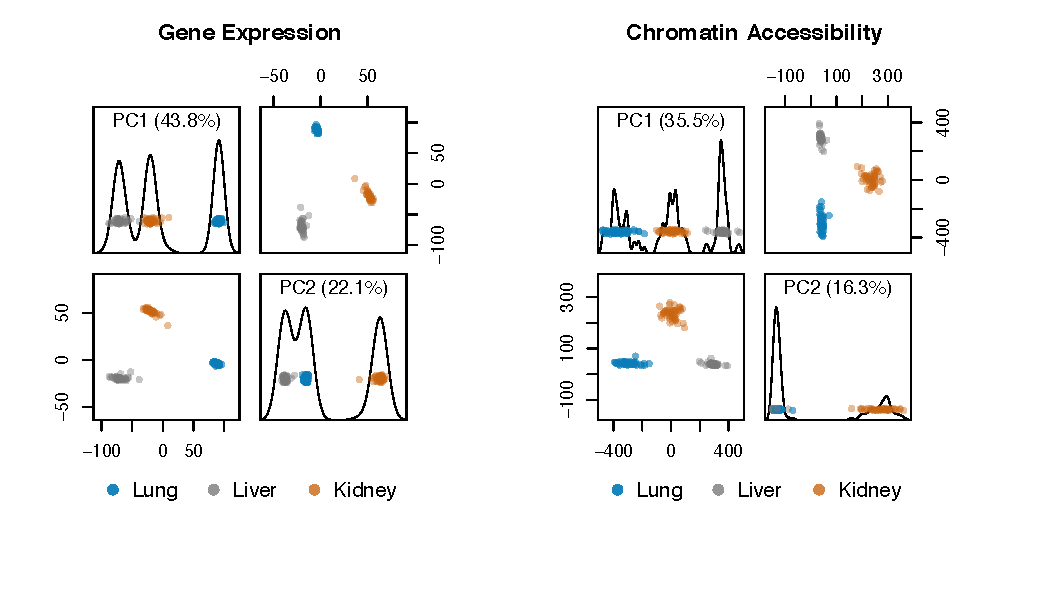
\includegraphics[width=0.8\textwidth, trim={0in 0in 0in 0in}, clip]{figs/pca_plot.pdf}
\caption{\textbf{Principle components analysis identifies tissue type as key source of variation for gene expression and chromatin accessibility.} Molecular traits for liver (pink), lung (green), and kidney (orange) tissue samples were derived from RNA-seq and ATAC-seq data. Principal components (PC) 1 and 2 capture a majority of the variation and show a greater amount of between tissue variability than within tissue variability. \label{fig:pca_plots}}
\end{figure*}

\begin{figure*}[hp]
\renewcommand{\familydefault}{\sfdefault}\normalfont
\centering
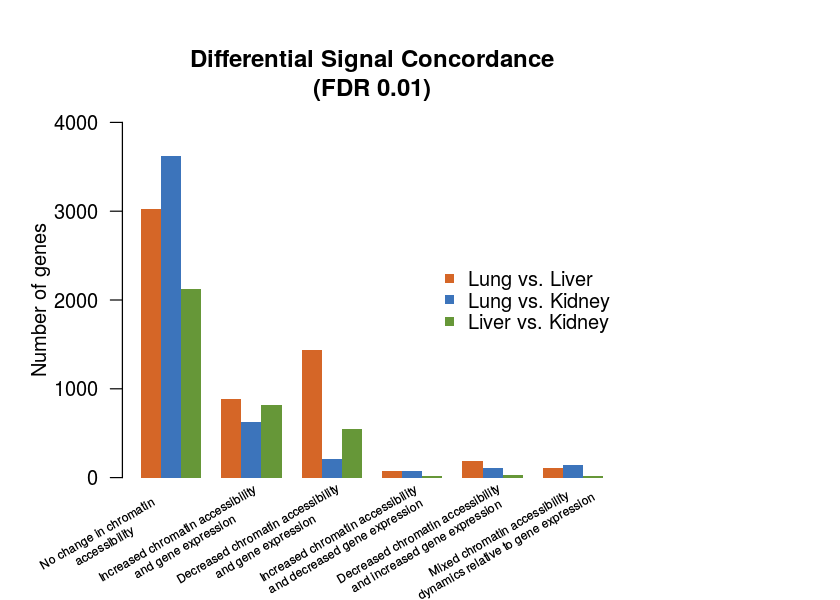
\includegraphics[width=0.8\textwidth, trim={0in 0in 0in 0in}, clip]{figs/diff_concordance.png}
\caption{\textbf{Concordance between differentially expressed (DE) genes and differentially accessible regions (DAR) in between-tissue comparisons.} Genes were categorized by the direction of the difference in expression and chromatin accessibility in their promoter regions.\label{fig:diff_concordance}}
\end{figure*}

\begin{figure*}[hp]
\renewcommand{\familydefault}{\sfdefault}\normalfont
\centering
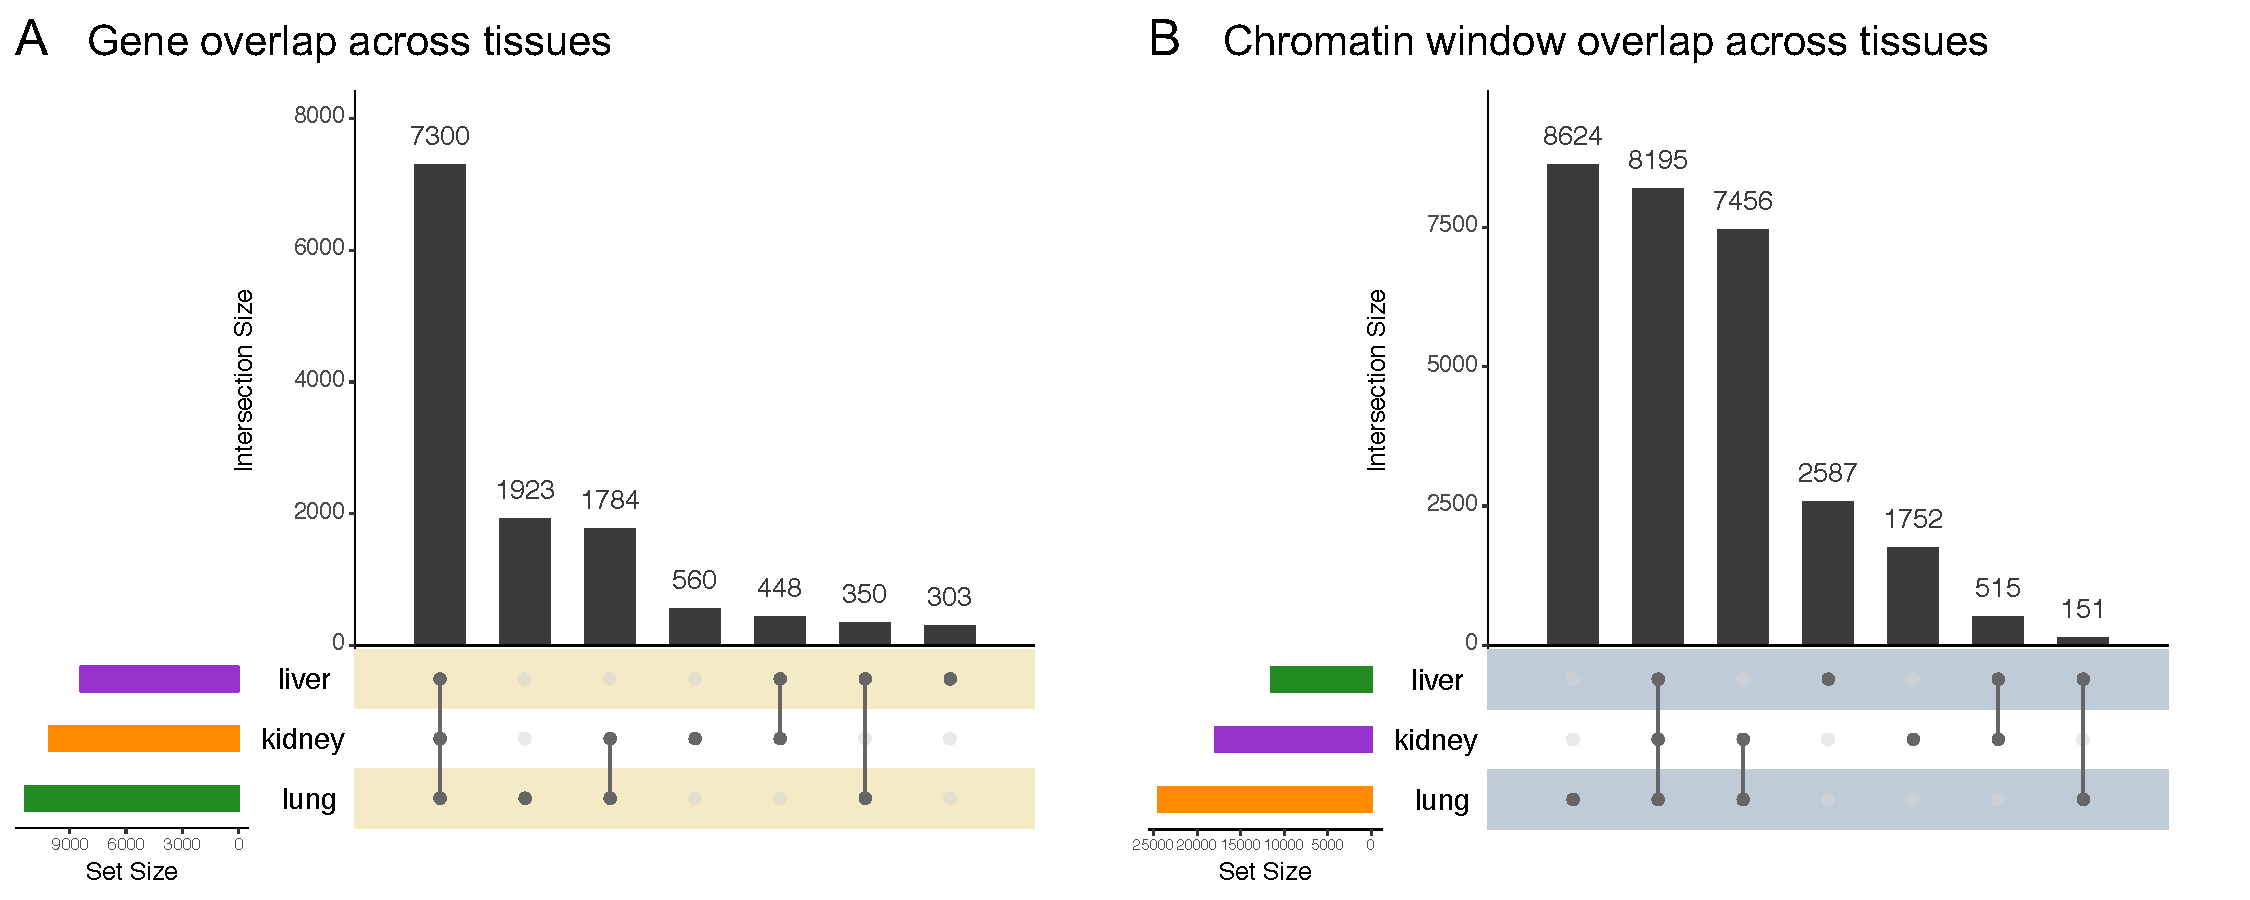
\includegraphics[width=\textwidth, trim={0in 0in 0in 0in}, clip]{figs/upset_genes_chromatin.pdf}
\caption{\textbf{Overlap across tissues of genes (A) and chromatin windows (B) used for QTL analysis.} Sequence traits were filtered to remove outcomes more likely to cause in spurious QTL signal. Genes with TPM $\le 1$ and chromatin windows with TMP $\le 5$ for $\ge$ 50\% of samples were removed from analysis. After this filtering process, lung had the greatest number of traits analyzed, for both genes and chromatin windows, followed by kidney and then liver. 
\label{fig:upset_genes_chromatin}}
\end{figure*}

\clearpage

\begin{figure*}[hp]
\renewcommand{\familydefault}{\sfdefault}\normalfont
\centering
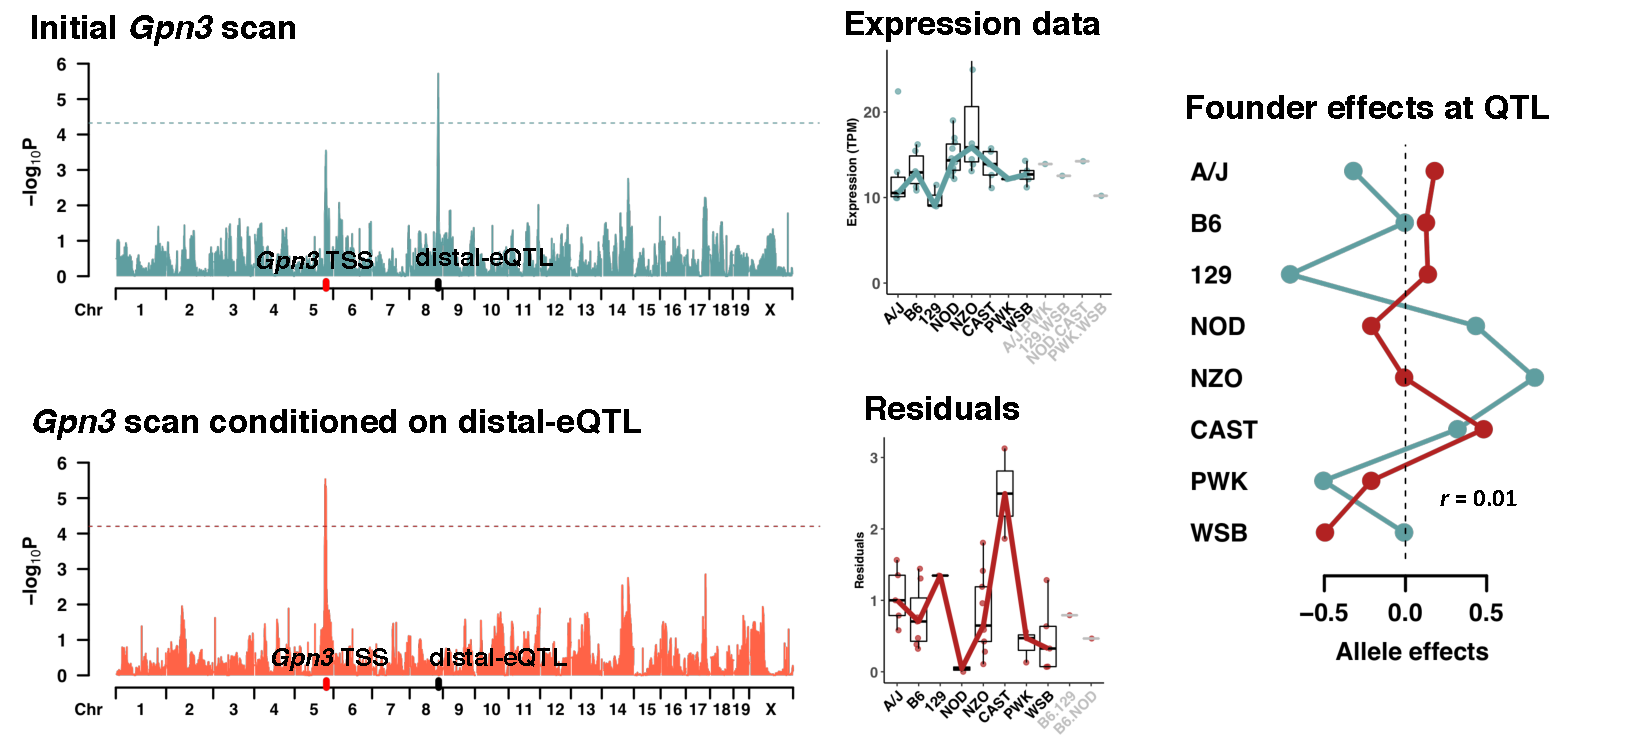
\includegraphics[width=\textwidth, trim={0in 0in 0in 0in}, clip]{figs/gpn3_conditional_scan.pdf}
\caption{\textbf{Detection of local-eQTL after conditioning on distal-eQTL for \textit{Gpn3}.} The multi-stage conditional regression approach of Analysis G allows for the detection of multiple genome-wide significant QTL, which can then be appropriately incorporated into a FDR procedure across many outcomes. In this example in lung tissue, the gene \textit{Gpn3} initially has a strong distal-eQTL on chromosome 8 (A). Though a peak is detected near the TSS of \textit{Gpn3}, it does not meet genome-wide significance. However, after conditioning on the distal-eQTL, the local-eQTL is detected (B). Horizontal dashed lines represent empirical 95\% significance thresholds based on 1000 permutations.
\label{fig:conditional_scans}}
\end{figure*}

\begin{figure*}[hp]
\renewcommand{\familydefault}{\sfdefault}\normalfont
\centering
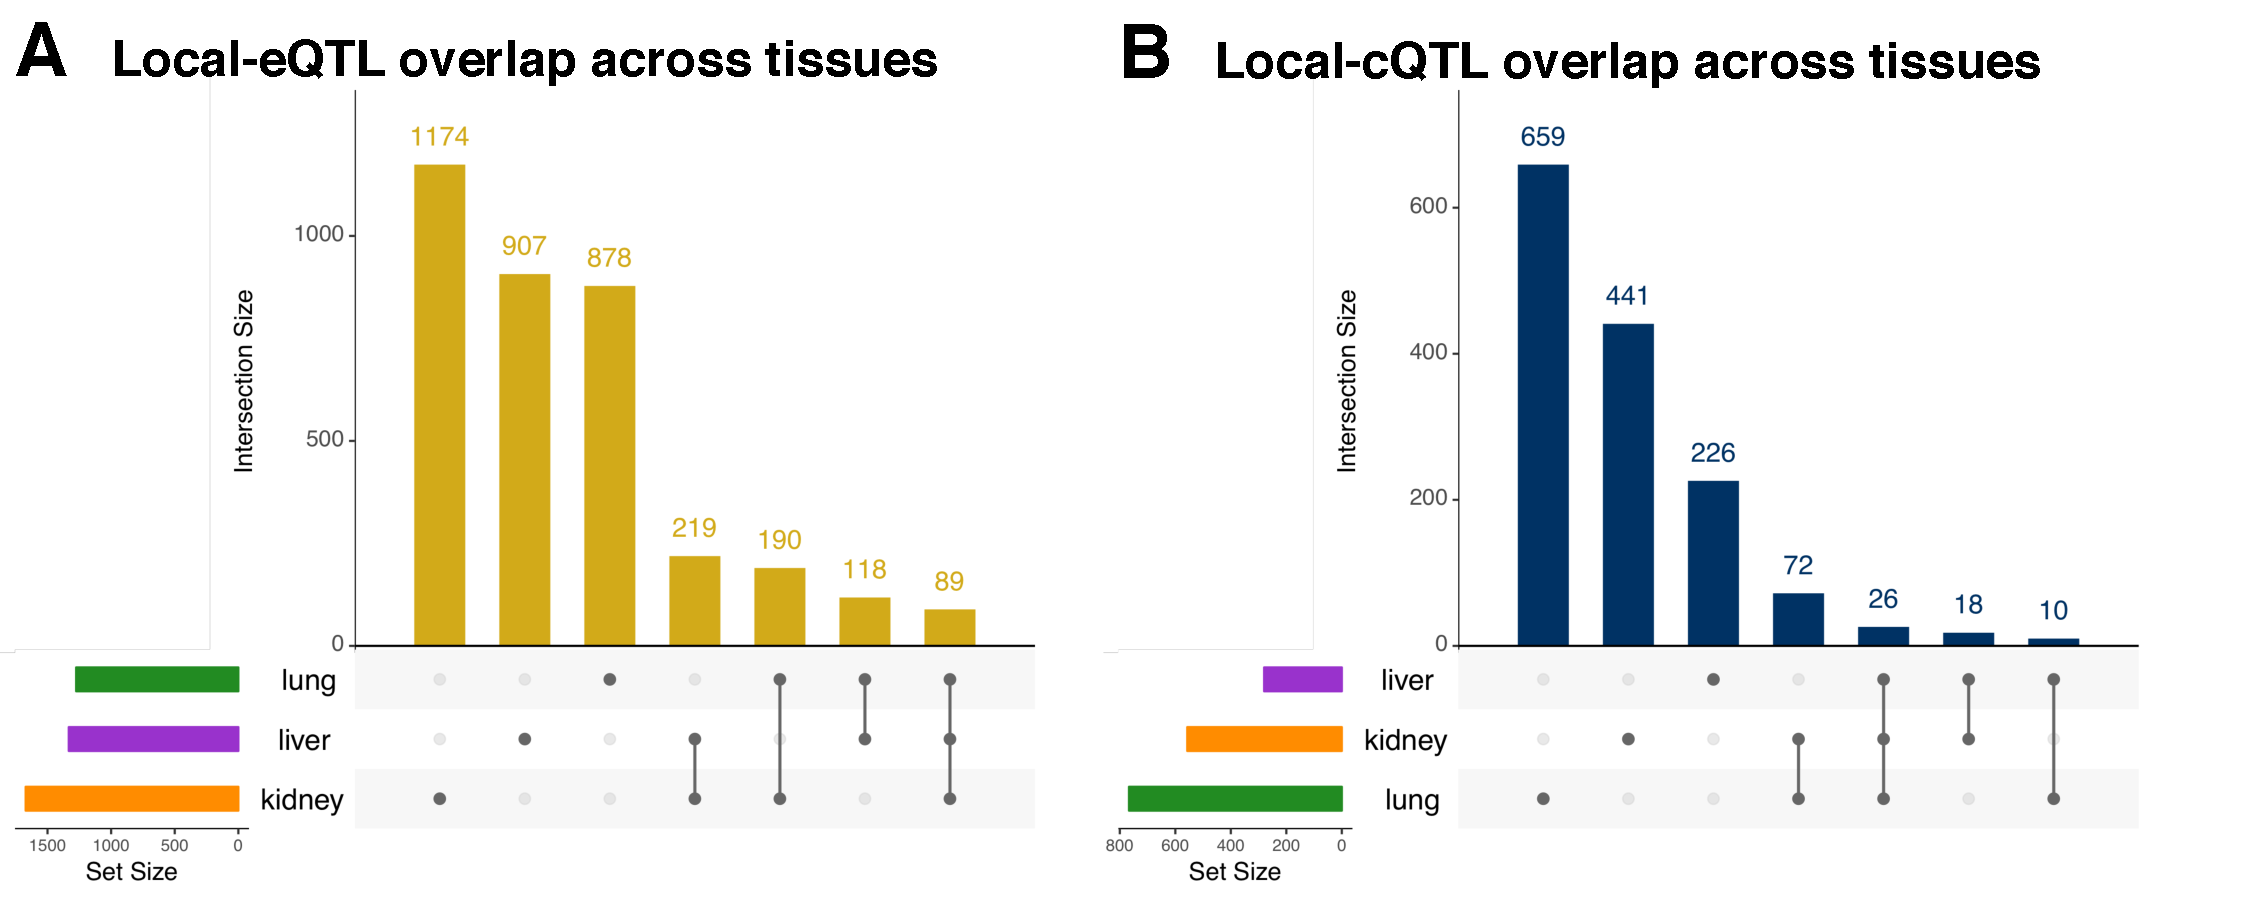
\includegraphics[width=\textwidth, trim={0in 0in 0in 0in}, clip]{figs/upset_eqtl_cqtl.pdf}
\caption{\textbf{Overlap across tissues of genes (A) and chromatin windows (B) with local-QTL detected.} The majority of sequence traits with a local-QTL detected were identified in only a single tissue. Kidney had the highest number of local-eQTL, whereas lung had the highest number of local-cQTL. Liver had a relative lack of local-cQTL, which may relate to its having the fewest chromatin windows analyzed (\textbf{Figure \ref{fig:upset_genes_chromatin}B}). Results included local-QTL detected with Analysis G (FDR < 0.1), Analysis LC (FDR < 0.1), and Analysis L (genome-wide and chromosome-wide). 
\label{fig:upset_eqtl_cqtl}}
\end{figure*}

\begin{figure*}[h]
\renewcommand{\familydefault}{\sfdefault}\normalfont
\centering
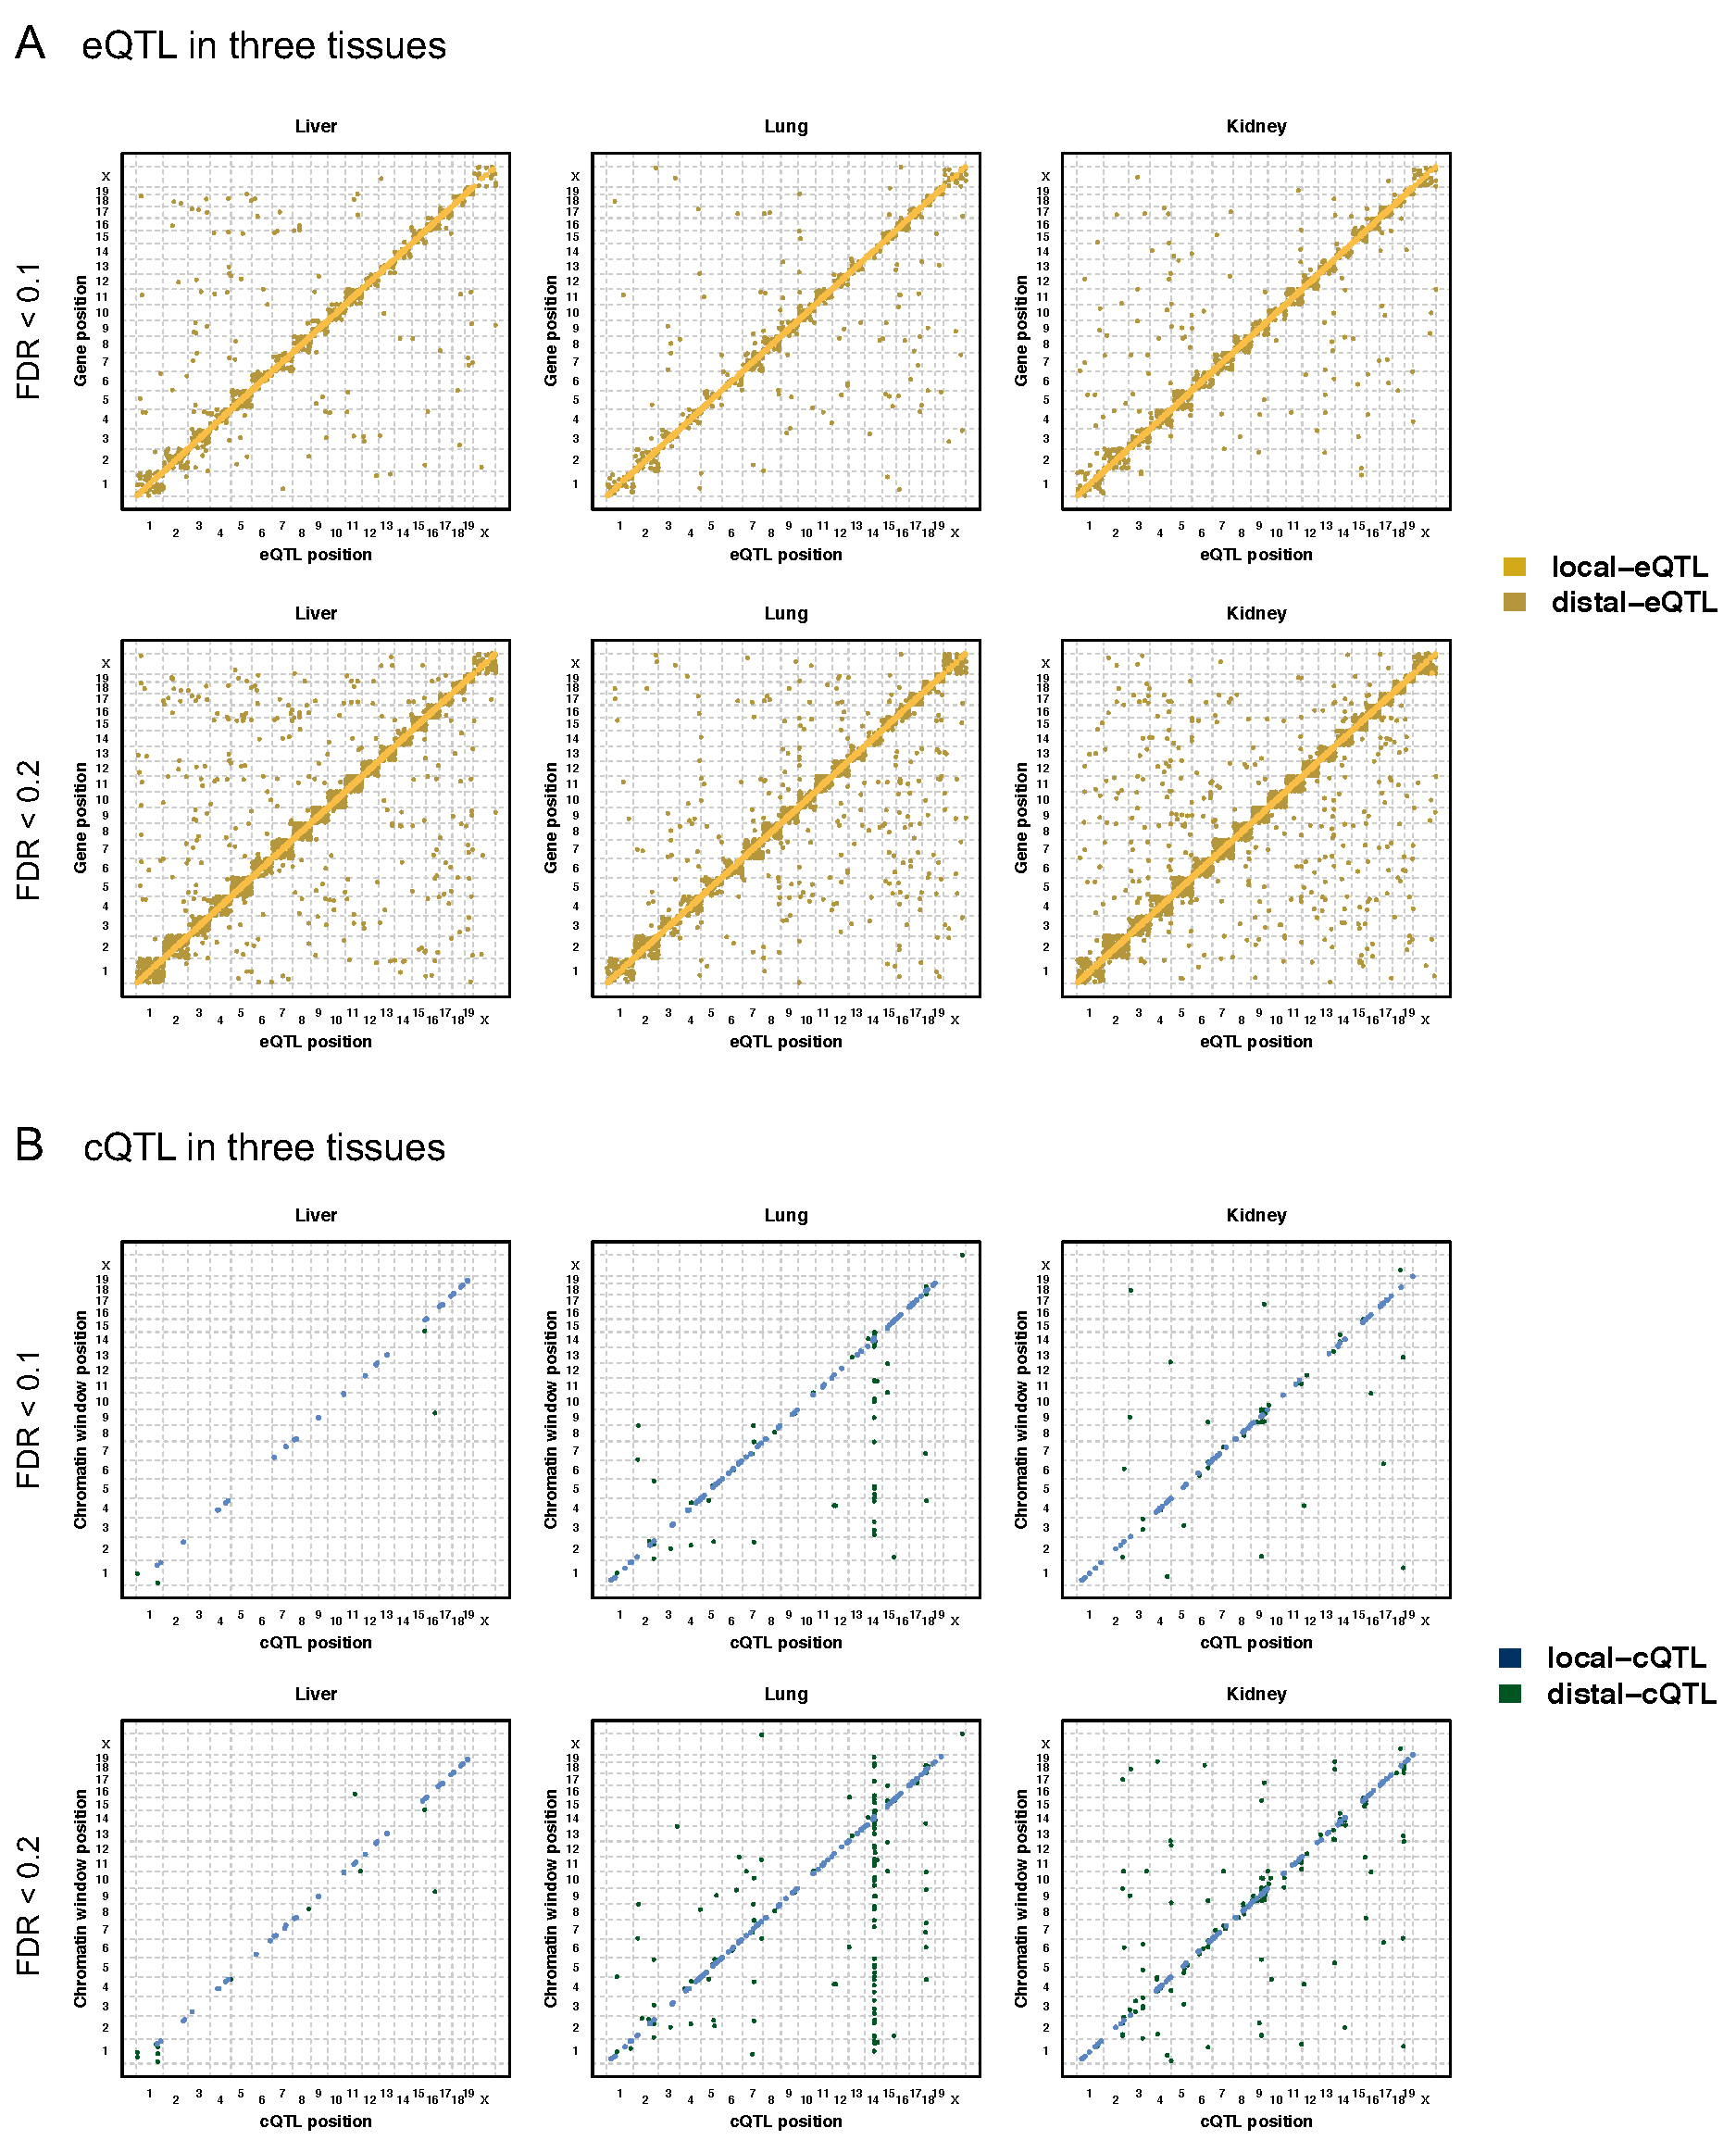
\includegraphics[width=0.8\textwidth, trim={0in 1.5in 0in 0in}, clip]{figs/qtl_map_supplemental.pdf}
\caption{\textbf{QTL mapping results using only Analysis G or Analysis LC.} QTL map plots of eQTL (A) and cQTL (B) with FDR controlled at 0.1 and 0.2 for liver, lung, and kidney. Detected QTL from Analysis G (multi-stage FDR) and Analysis LC (chromosome-wide FDR) are included. Analysis LC, which uses FDR control for chromosome-wide significant QTL, produces a large number of intra-chromosomal distal QTL. The y-axis represents the genomic position of the gene or chromatin site, and the x-axis represents the genomic position of the QTL. Local-QTL appear as dots along the diagonal.
\label{fig:grid_fdr_plot}}
\end{figure*}

\begin{figure*}[h]
\centering
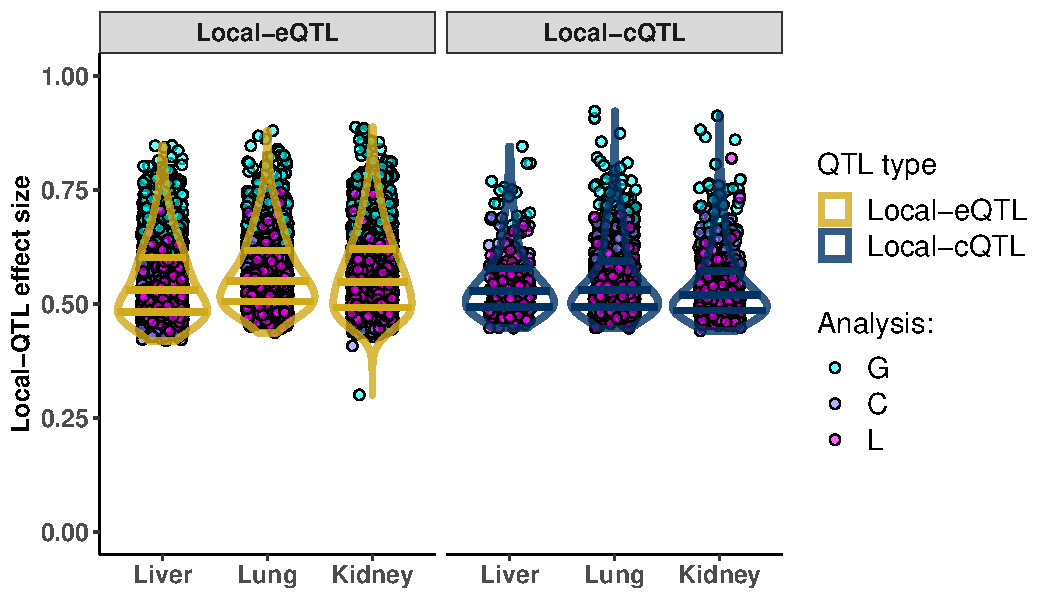
\includegraphics[width=\textwidth, trim={0in 0in 0in 0in}, clip]{figs/local_qtl_effects.pdf}
\caption{\textbf{Local-QTL effect sizes by mapping analysis.} Based on ranking mapping analyses with respect to the extent of scope, local (L; purple) to local-chromosome (LC; orange) to genome-wide (G; green), the greater the scope corresponded to reduced power to detect QTL, shown in liver, lung, and kidney tissues for gene expression (yellow line) and chromatin accessibility (blue line). Each dot represents a detected local-QTL, colored according to the highest scope mapping procedure that detected it. The three horizontal bars represent the 25\textsuperscript{th}, 50\textsuperscript{th}, and 75\textsuperscript{th} quantiles of QTL effect sizes for all local-QTL per tissue. Analysis G generally detects QTL with effect size > 60\%, whereas Analyses LC and L detect QTL effect sizes > 45\%. Effect size estimates correspond to a fixed effects model of the QTL.
\label{fig:qtl_effect_sizes_by_method}}
\end{figure*}

%\begin{figure*}[h]
%\centering
%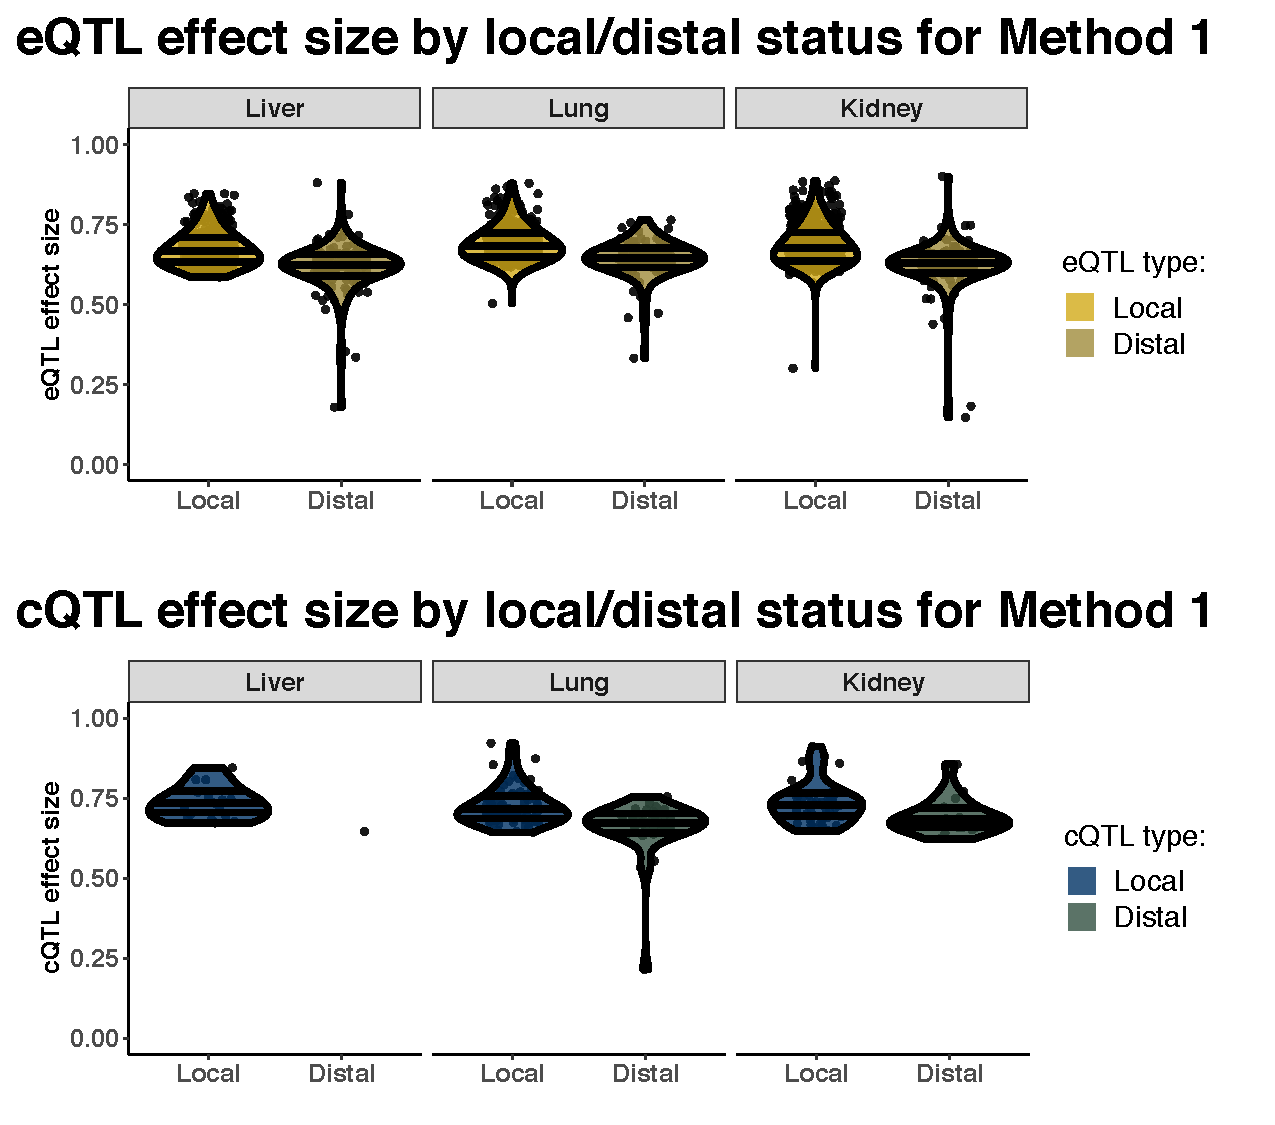
\includegraphics[width=0.9\textwidth, trim={0in 0in 0in 0in}, clip]{figs/qtl_effect_sizes_strict.pdf}
%\caption{\textbf{QTL effect sizes by local/distal status for Analysis G.} Each dot represents a detected QTL through either Analysis G (FDR $\leq$ 0.1). The three horizontal bars represent the 25\textsuperscript{th}, 50\textsuperscript{th}, and 75\textsuperscript{th} quantiles of QTL effect sizes for all local-QTL per tissue. More local-QTL are detected and have larger effects on average than the detected distal-QTL, in both gene expression and chromatin accessibility. Effect size estimates are based on a fixed effects model.
%\label{fig:qtl_effect_sizes_strict}}
%\end{figure*}
%
%\begin{figure*}[h]
%\centering
%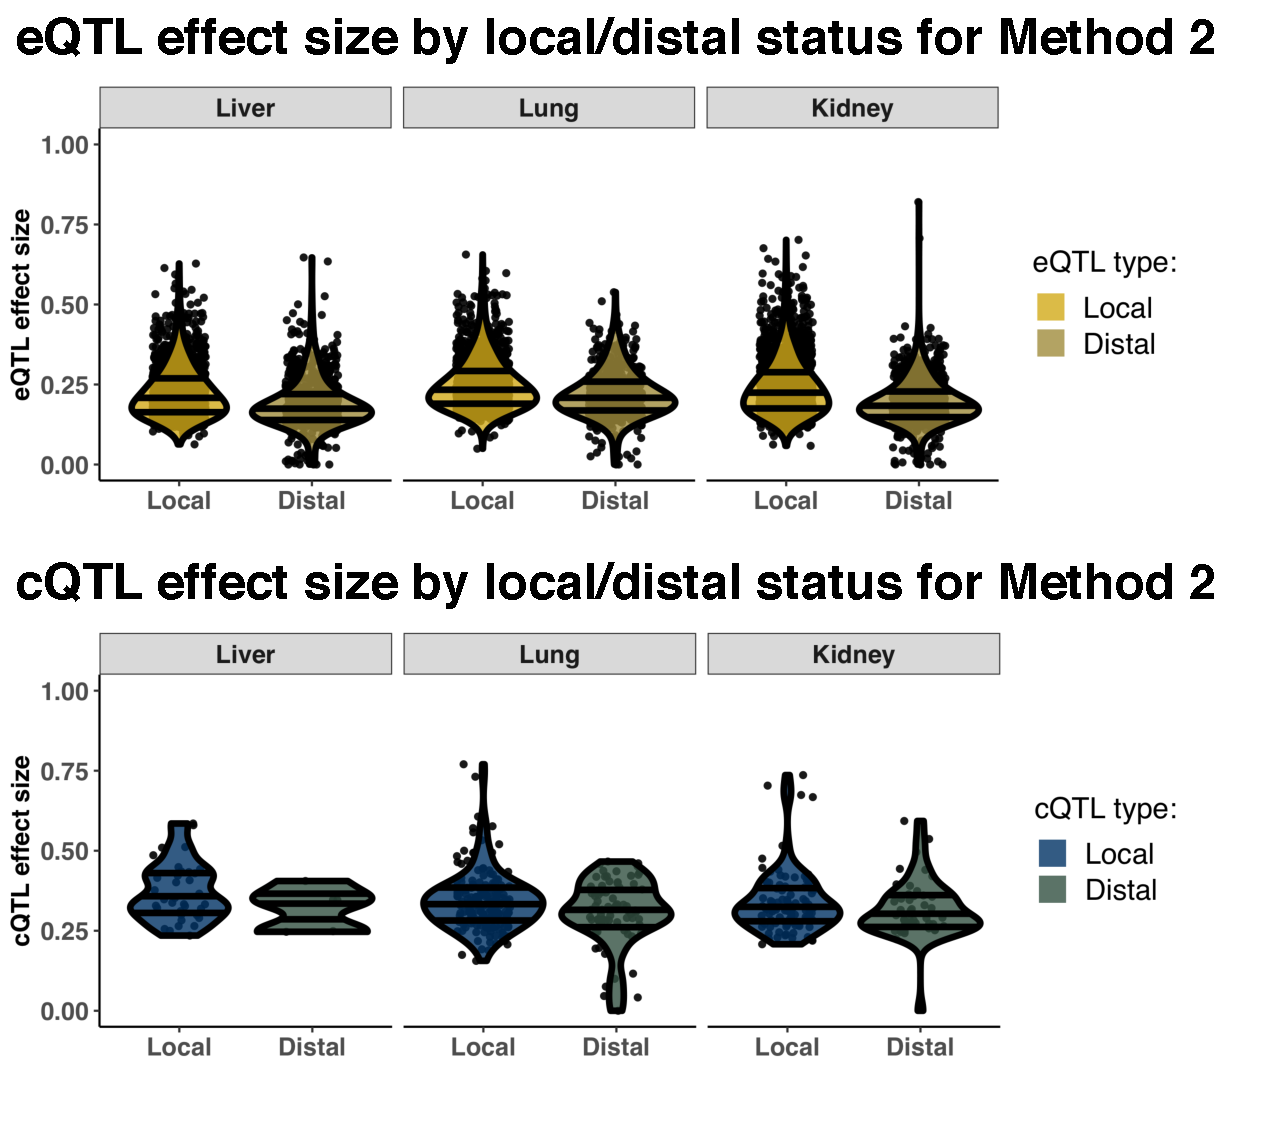
\includegraphics[width=0.9\textwidth, trim={0in 0.25in 0in 0in}, clip]{figs/qtl_effect_sizes_permissive.pdf}
%\caption{\textbf{QTL effect sizes by local/distal status for Analyses G and LC.} Each dot represents a QTL detected through either Analyses G or LC (FDR $\leq$ 0.1). The three horizontal bars represent the 25\textsuperscript{th}, 50\textsuperscript{th}, and 75\textsuperscript{th} quantiles of QTL effect sizes for all local-QTL per tissue. Consistent with Analysis G results, more local-eQTL are detected and have higher effects than distal-QTL. Analysis LC detects a large number of intra-chromosomal distal-QTL that Analysis G does not, many of which have low effect sizes. Effect size estimates are based on a fixed effects model.
%\label{fig:qtl_effect_sizes_permissive}}
%\end{figure*}

\begin{figure*}[h]
\centering
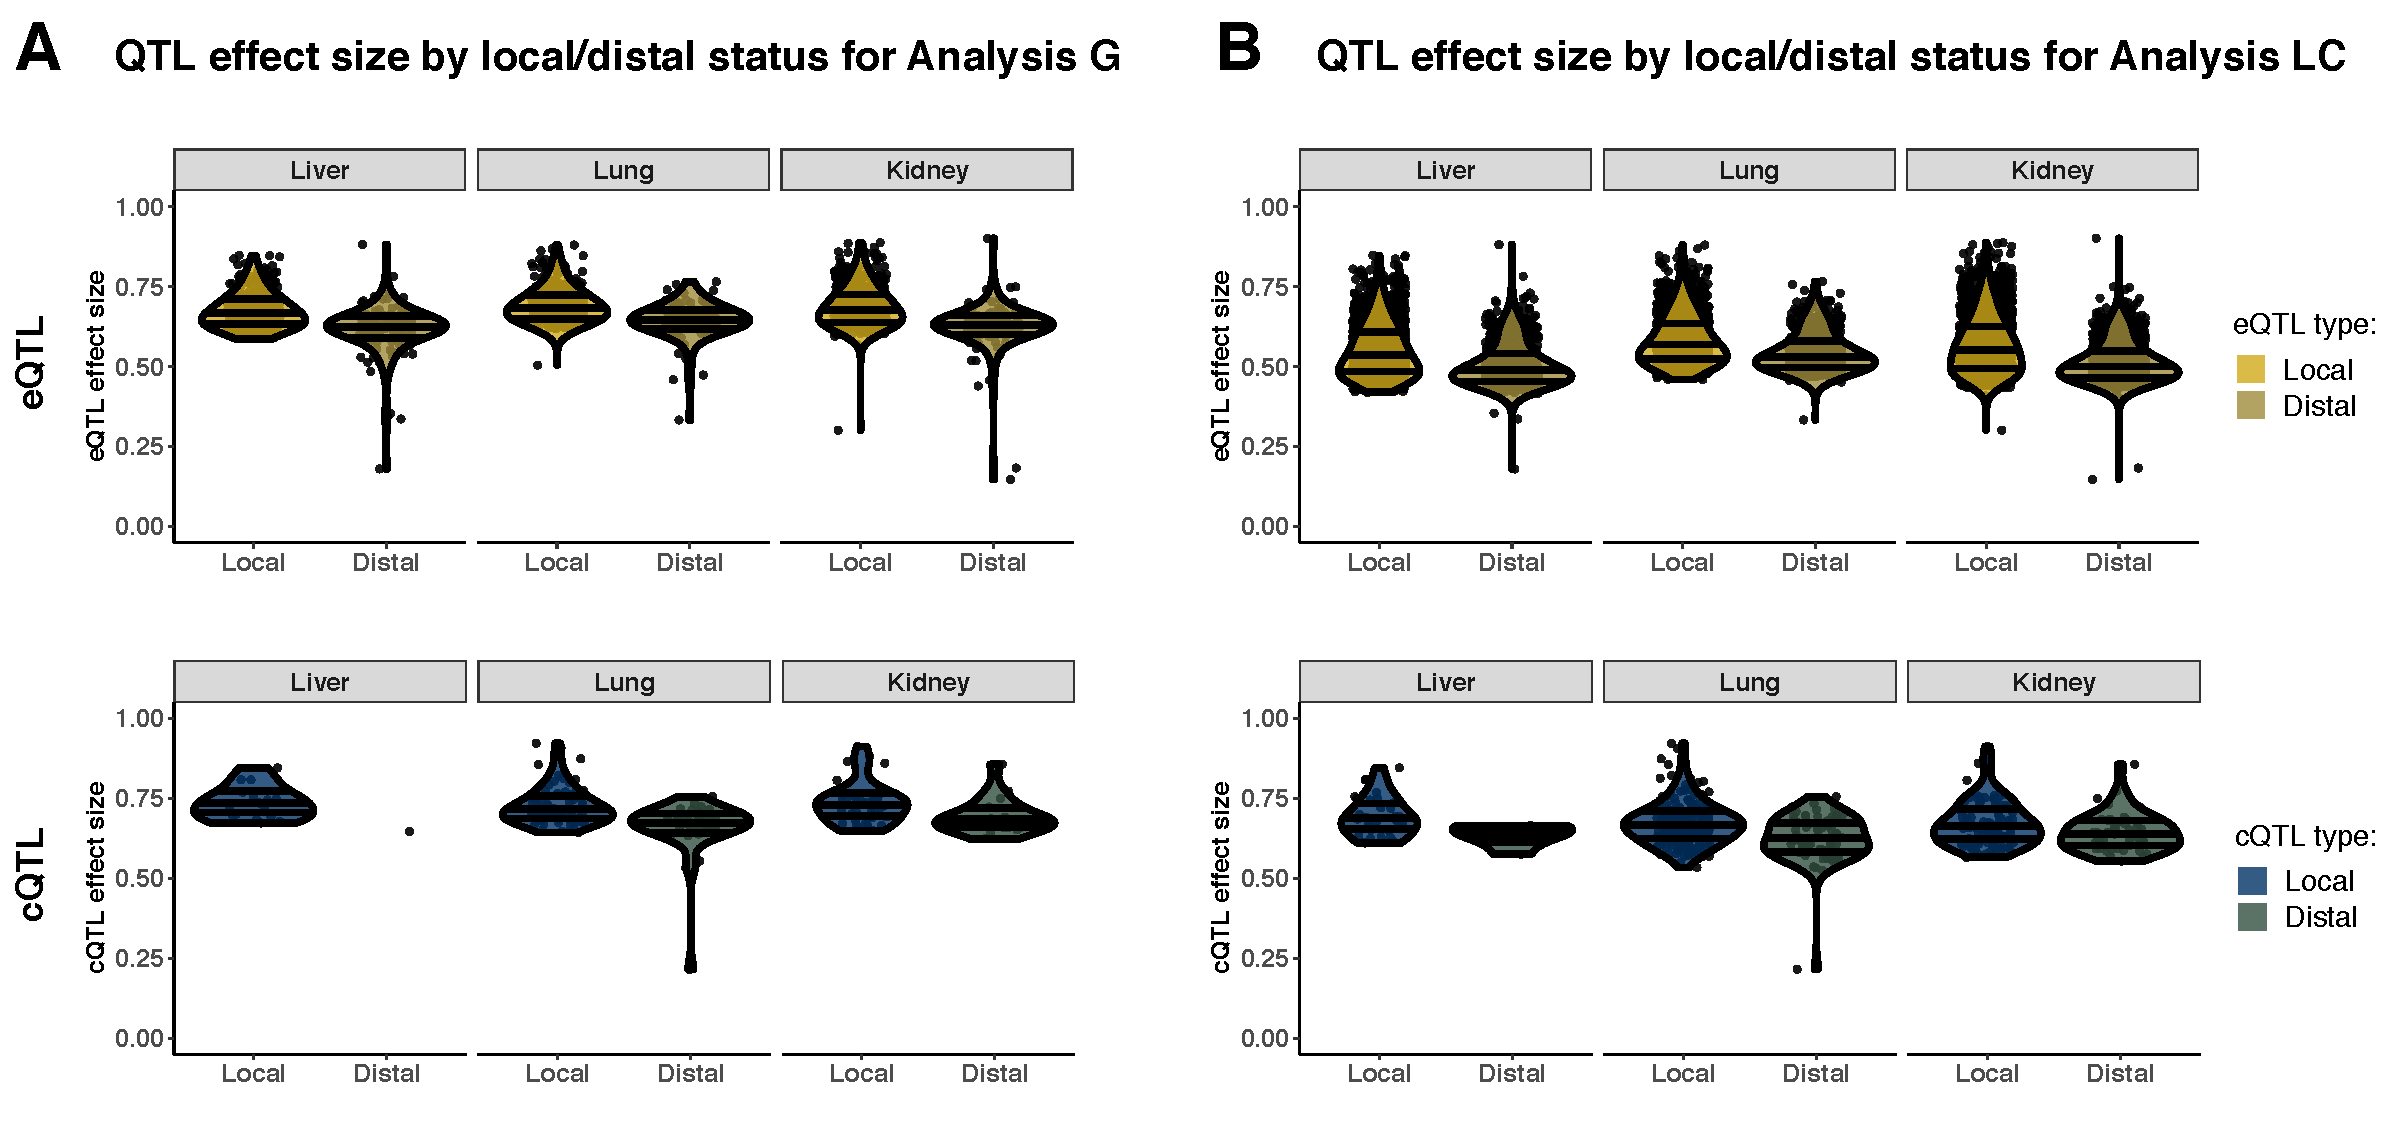
\includegraphics[width=0.9\textwidth, trim={0in 0.25in 0in 0in}, clip]{figs/qtl_effect_sizes_local_v_distal.pdf}
\caption{\textbf{QTL effect sizes by local/distal status.} Each dot represents a QTL detected through either Analyses G (A) or LC (B) with FDR $\leq$ 0.1. The three horizontal bars represent the 25\textsuperscript{th}, 50\textsuperscript{th}, and 75\textsuperscript{th} quantiles of QTL effect sizes for all local-QTL per tissue. More local-eQTL are detected and have higher effects than distal-QTL. Analysis LC detects a large number of intra-chromosomal distal-QTL that Analysis G does not, many of which have low effect sizes. Effect size estimates are based on a fixed effects model.
\label{fig:qtl_effect_sizes_local_v_distal}}
\end{figure*}

\begin{figure*}[h]
\centering
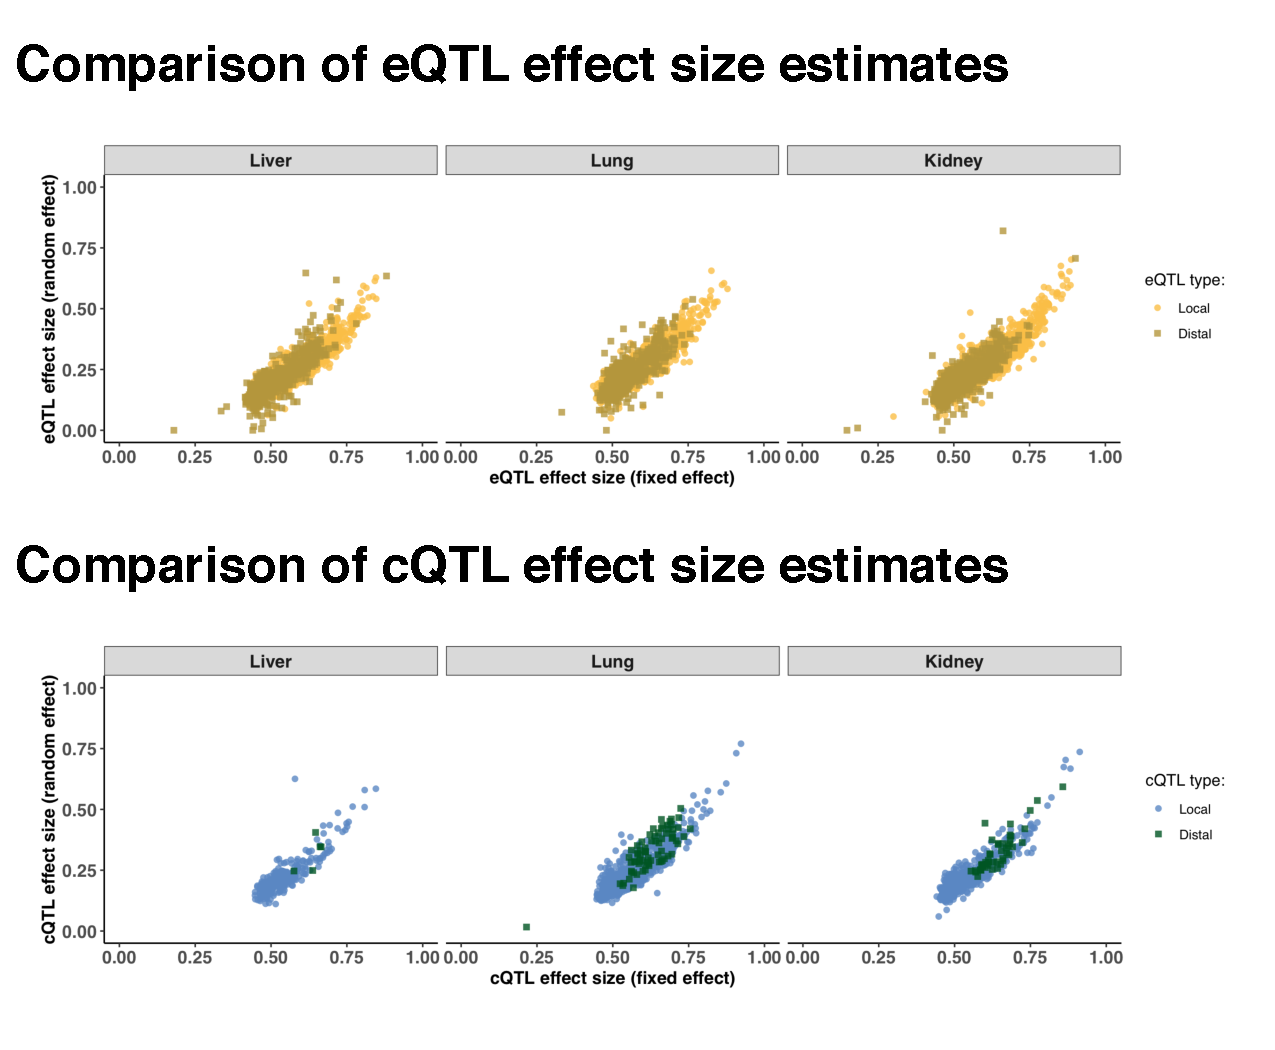
\includegraphics[width=0.9\textwidth, trim={0in 0in 0in 0in}, clip]{figs/fixefvsranef_qtl.pdf}
\caption{\textbf{Comparison of QTL effect sizes estimates from fixed effects and random effects models.} The effect size corresponding to the random effect fit is harshly penalized compared to the fixed effect estimate, likely due to a small sample size of 47 individuals. Notably, there are a number of distal-eQTL that are more harshly reduced by the random effects model compared to the other QTL, likely representing signals resulting from extreme observations or imbalances in founder contributions at the locus. QTL detected by Analysis G (FDR $\le 0.1$), 2 (FDR $\le 0.1$), and 3 are shown.
\label{fig:qtl_effect_size_fixefvsranef}}
\end{figure*}

%\begin{figure*}[hp]
%\renewcommand{\familydefault}{\sfdefault}\normalfont
%\centering
%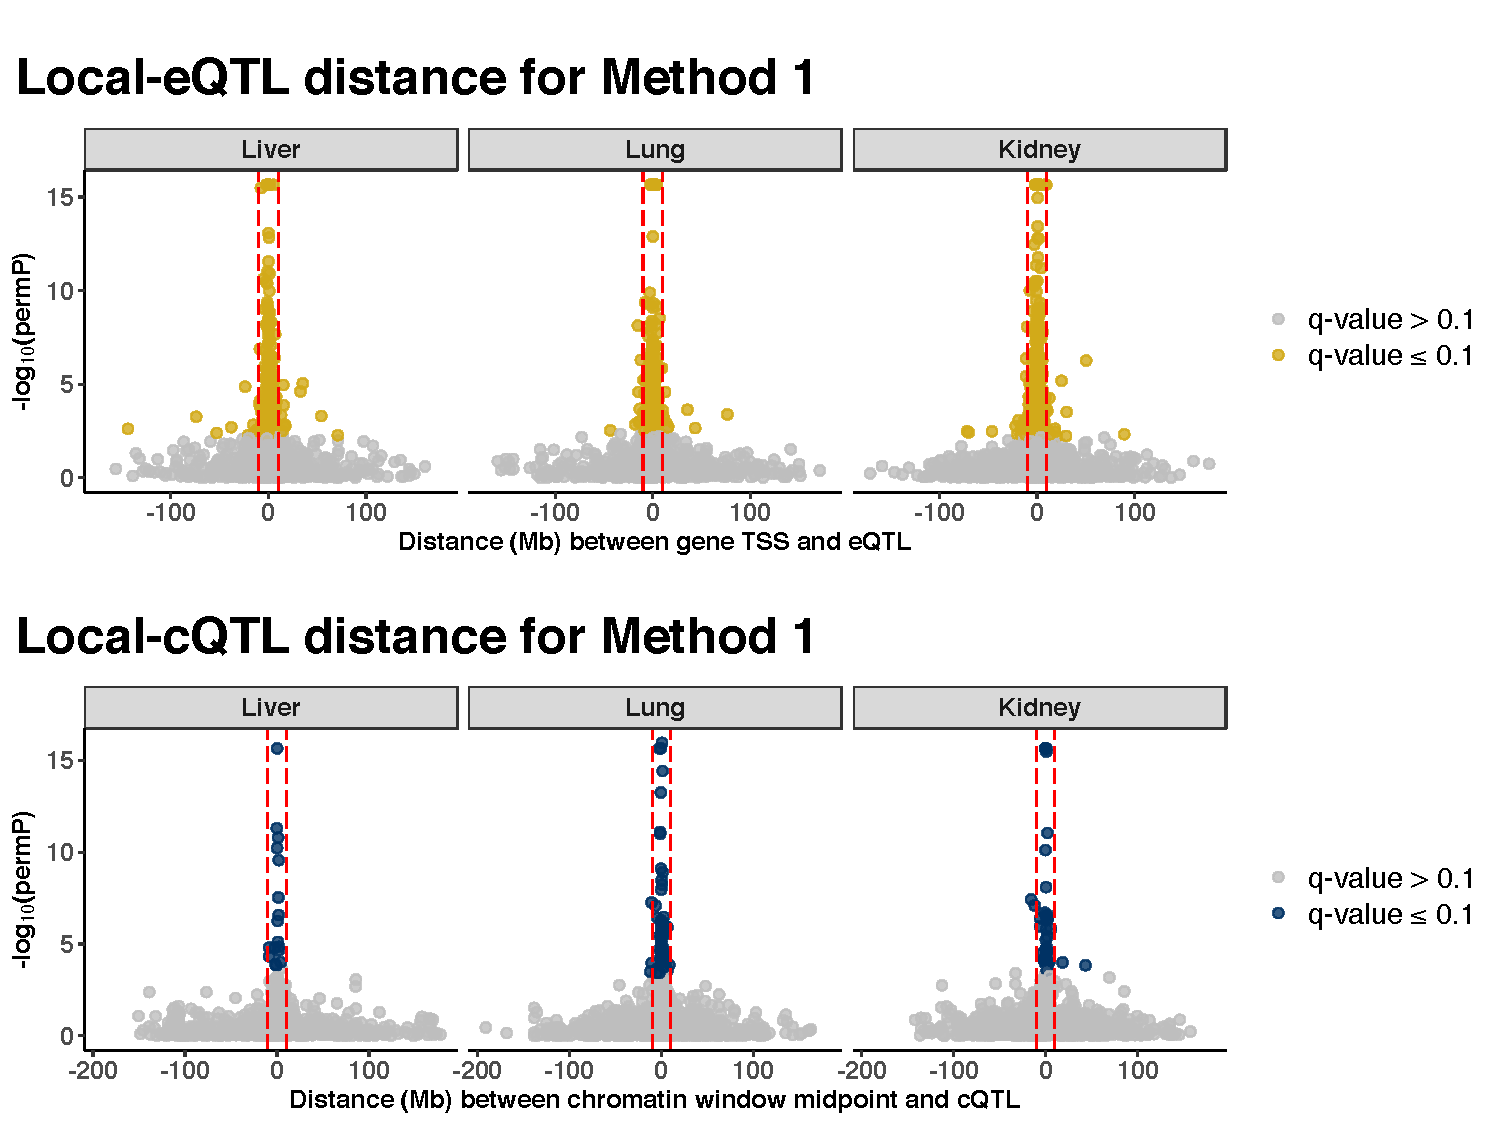
\includegraphics[width=0.9\textwidth]{figs/qtl_distance_method1.pdf}
%\caption{\textbf{Highly significant QTL are proximal to gene TSS and chromatin window midpoint.} The genome-wide permutation-based $p$-value (permP) from Analysis G (first stage-only) for eQTL and cQTL compared to the distance (Mb) from the gene TSS and the midpoint of the chromatin site, respectively. Inter-chromosomal distal-QTL are not included. The red dashed lines represent 10Mb upstream and downstream of the gene TSS or the midpoint of the chromatin site for classifying QTL as local or distal. Significant signals (yellow or blue), based on $\text{q-value} \le 0.1$, are largely local. \label{fig:genomewide_dist}}
%\end{figure*}
%
%\clearpage
%
%\begin{figure*}[hp]
%\renewcommand{\familydefault}{\sfdefault}\normalfont
%\centering
%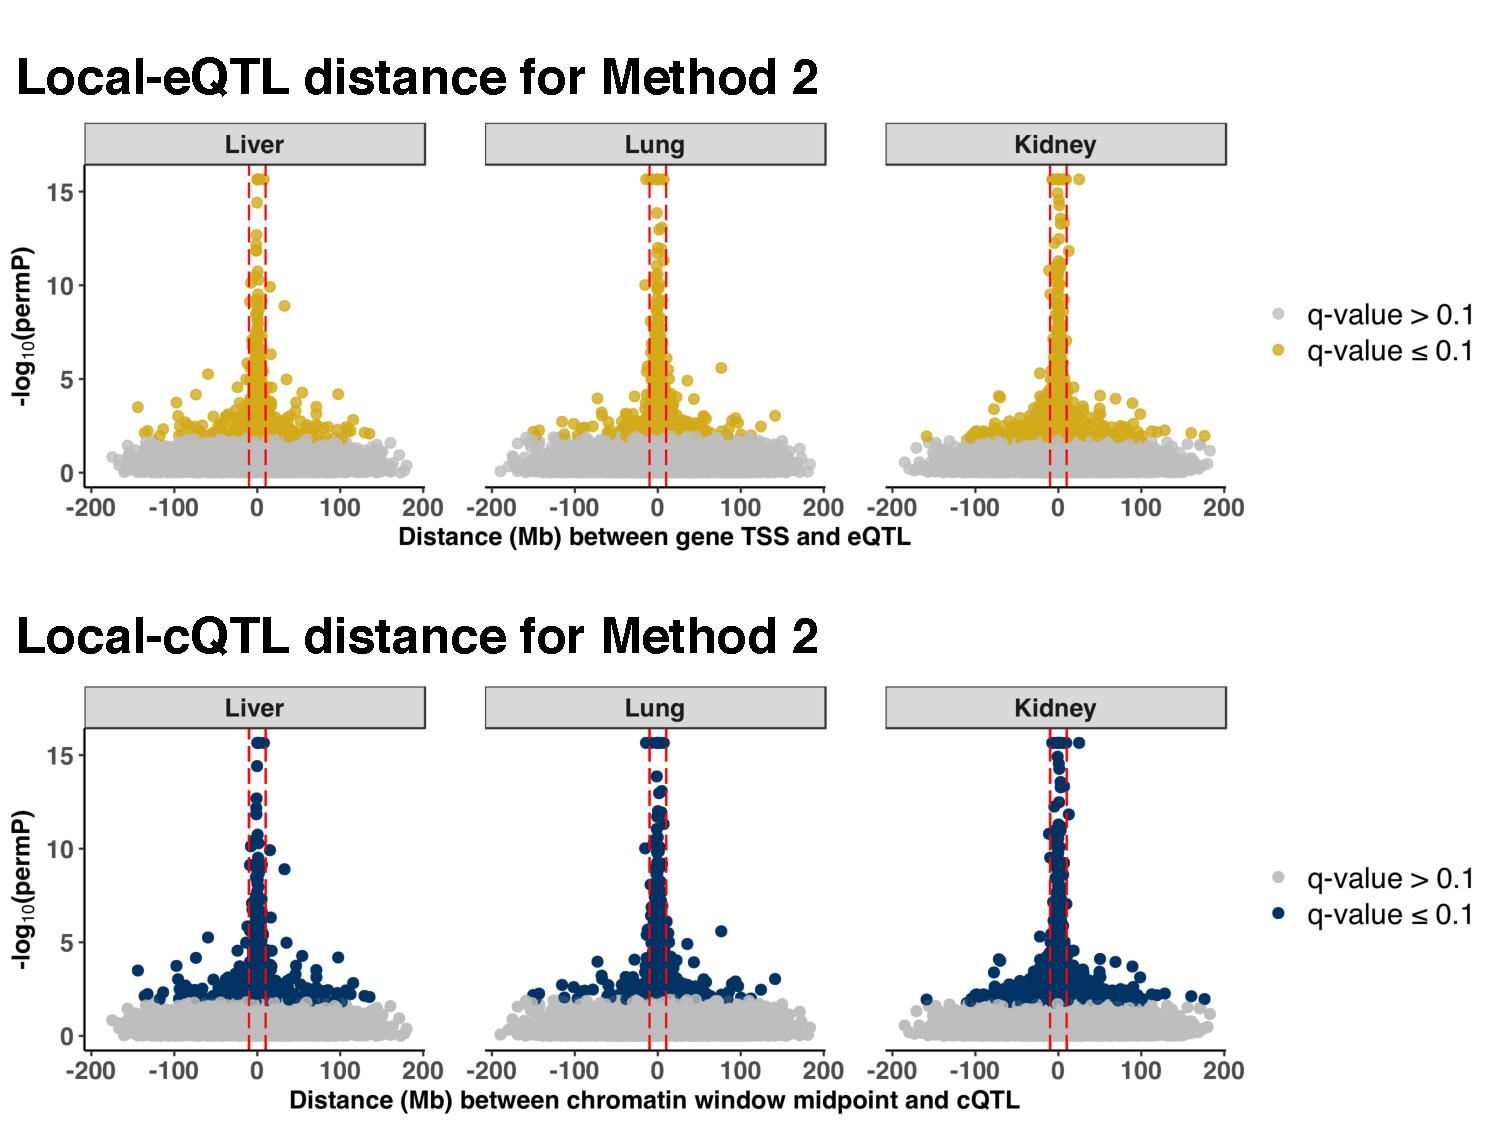
\includegraphics[width=0.9\textwidth]{figs/qtl_distance_method2.pdf}
%\caption{\textbf{Analyses that use chromosome-wide significance detect many putative intra-chromosomal distal-QTL.} The chromosome-wide permutation-based $p$-value (permP) from Analysis LC for eQTL and cQTL compared to distance (Mb) from the gene TSS and the midpoint of the chromatin site, respectively. Analysis LC is restricted to QTL on the local-chromosome. The red dashed lines represent 10Mb upstream and downstream of gene TSS or chromatin site for classifying an association as local or distal. Significant QTL (yellow or blue) are largely proximal.
%\label{fig:chrwide_dist}}
%\end{figure*}

\begin{figure*}[hp]
\renewcommand{\familydefault}{\sfdefault}\normalfont
\centering
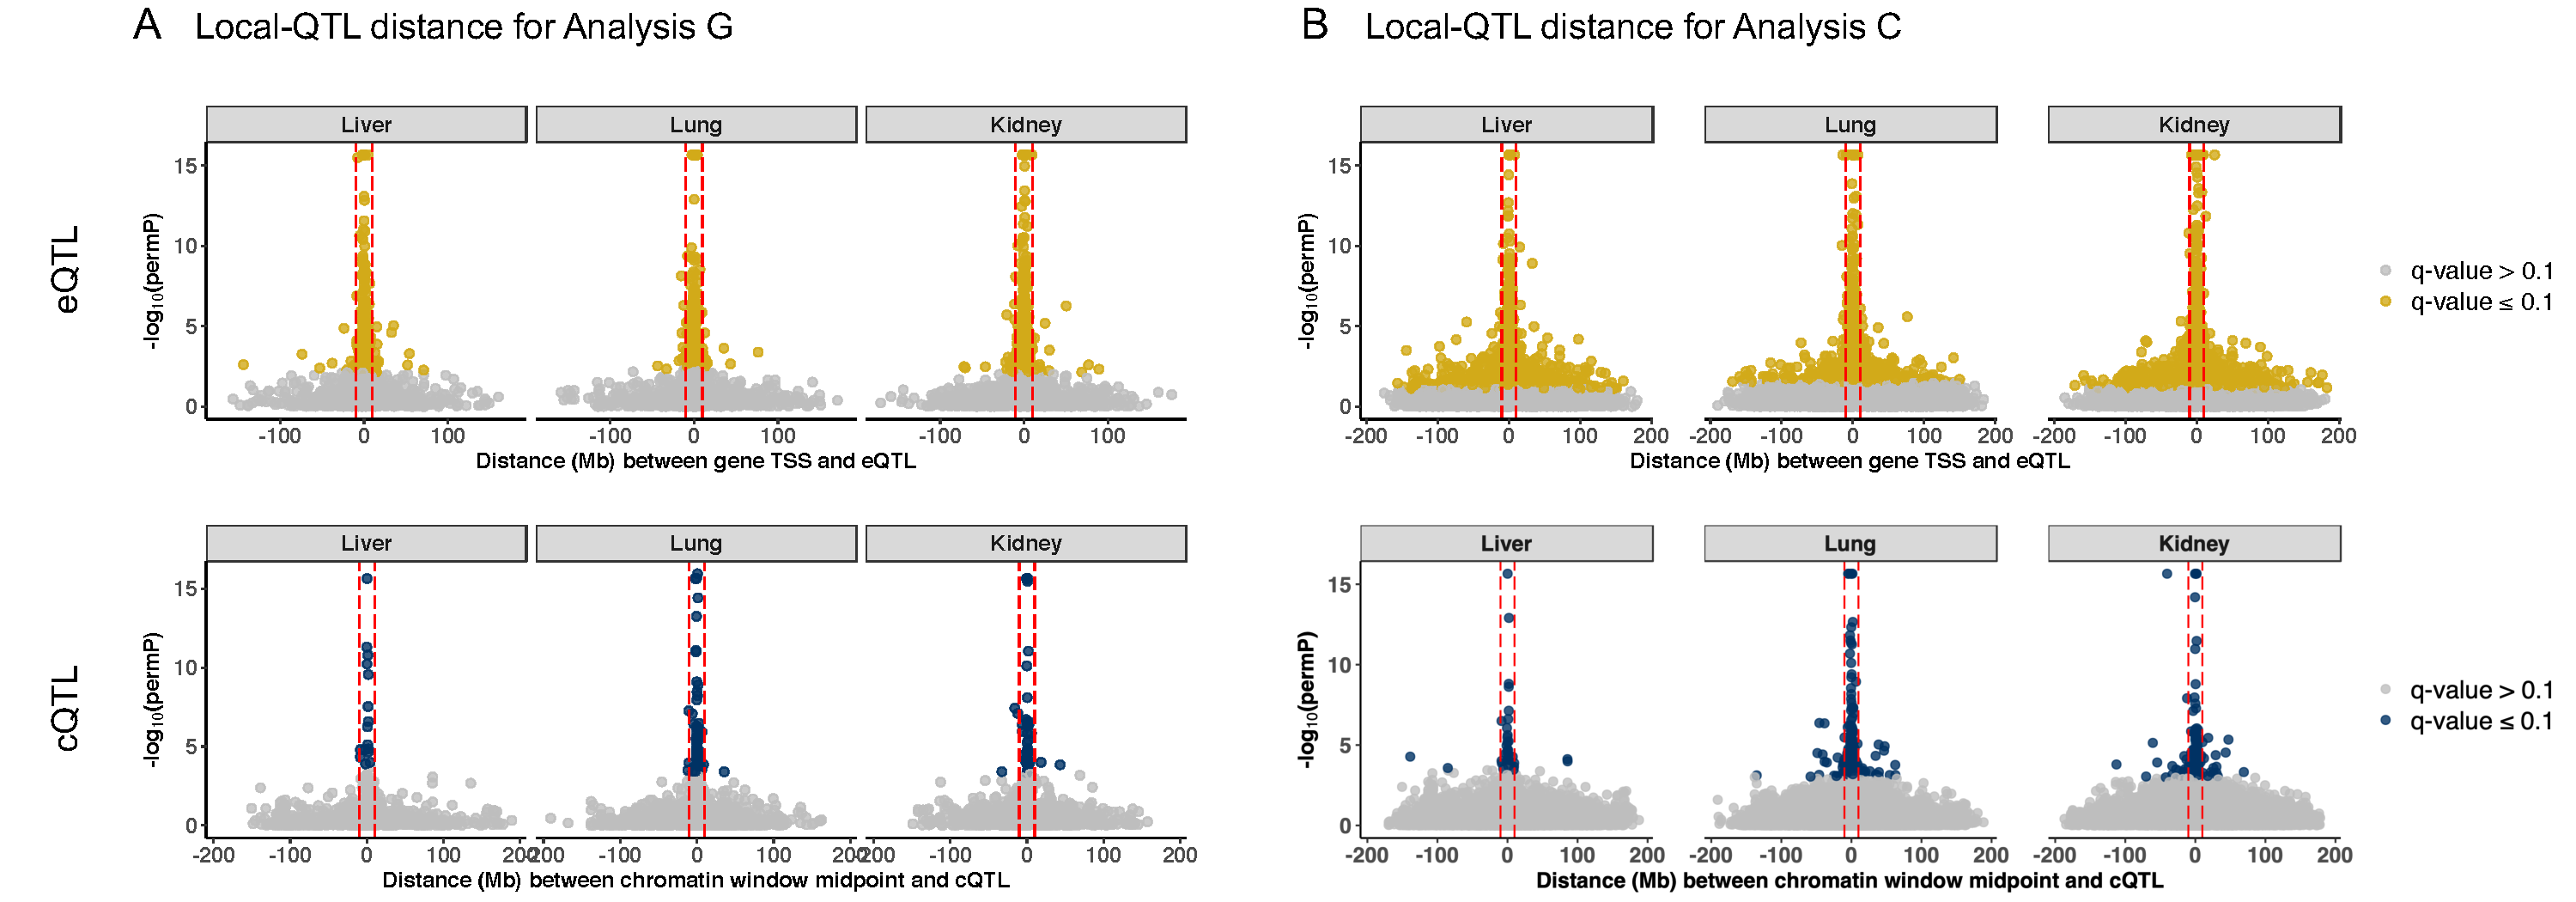
\includegraphics[width=\textwidth]{figs/qtl_distance_all.pdf}
\caption{\textbf{Highly significant QTL map nearby the gene TSS and chromatin window midpoint.} The permutation-based $p$-value (permP) from Analyses G (A) and LC (B) for eQTL and cQTL by the distance (Mb) from the gene TSS \textbf{[top]} and the midpoint of the chromatin site \textbf{[bottom]}. Inter-chromosomal distal-QTL are not included. The red dashed lines represent 10Mb upstream and downstream of the gene TSS or the midpoint of the chromatin site for classifying QTL as local or distal. Significant signals (yellow or blue), based on $\text{q-value} \le 0.1$, are largely local. Analysis LC detects many more intra-chromosomal distal-QTL.
\label{fig:dist_all}}
\end{figure*}

\begin{figure*}[hp]
\renewcommand{\familydefault}{\sfdefault}\normalfont
\centering
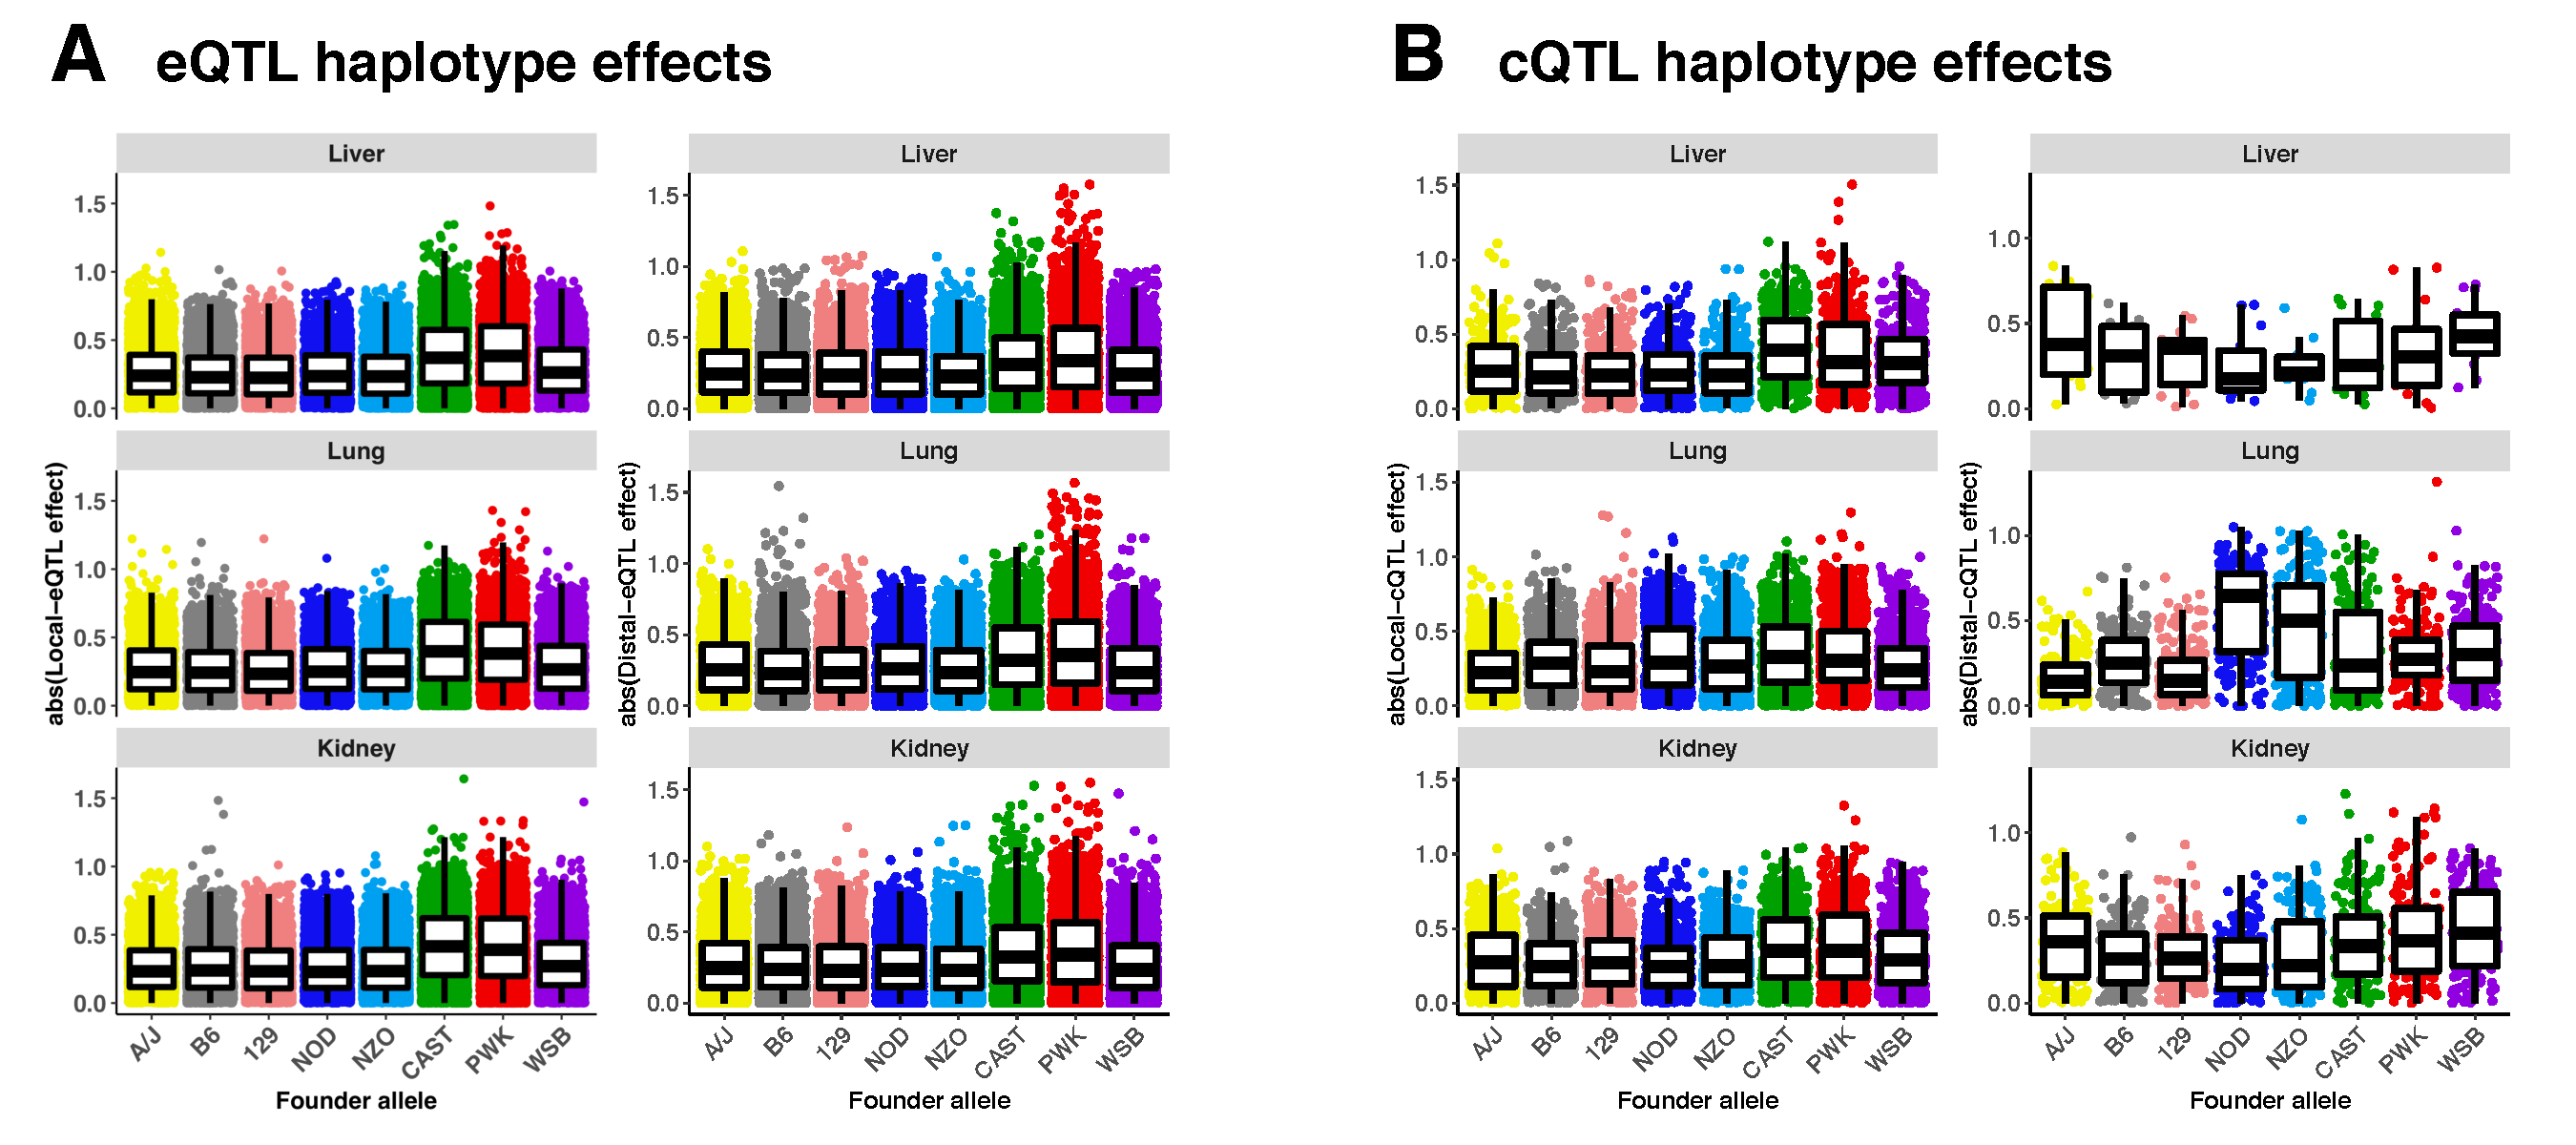
\includegraphics[width=\textwidth, trim={0in 0in 0in 0in}, clip]{figs/all_qtl_effects_abs.pdf}
\caption{\textbf{CAST and PWK haploytpes have more extreme haplotype effects for eQTL and cQTL compared with the other strains.} Haplotype effects were estimated as BLUPs, which are constrained and centered around 0. Each QTL is represented by an 8-element effect vector. Founders with more extreme effects are identified by comparing the absolute values of effects. Haploytpe effects for eQTL (A() are are similar to cQTL (B). Trends are unstable in distal-cQTL because so few are identified.
\label{fig:qtl_effects_abs}}
\end{figure*}

\begin{figure*}[hp]
\renewcommand{\familydefault}{\sfdefault}\normalfont
\centering
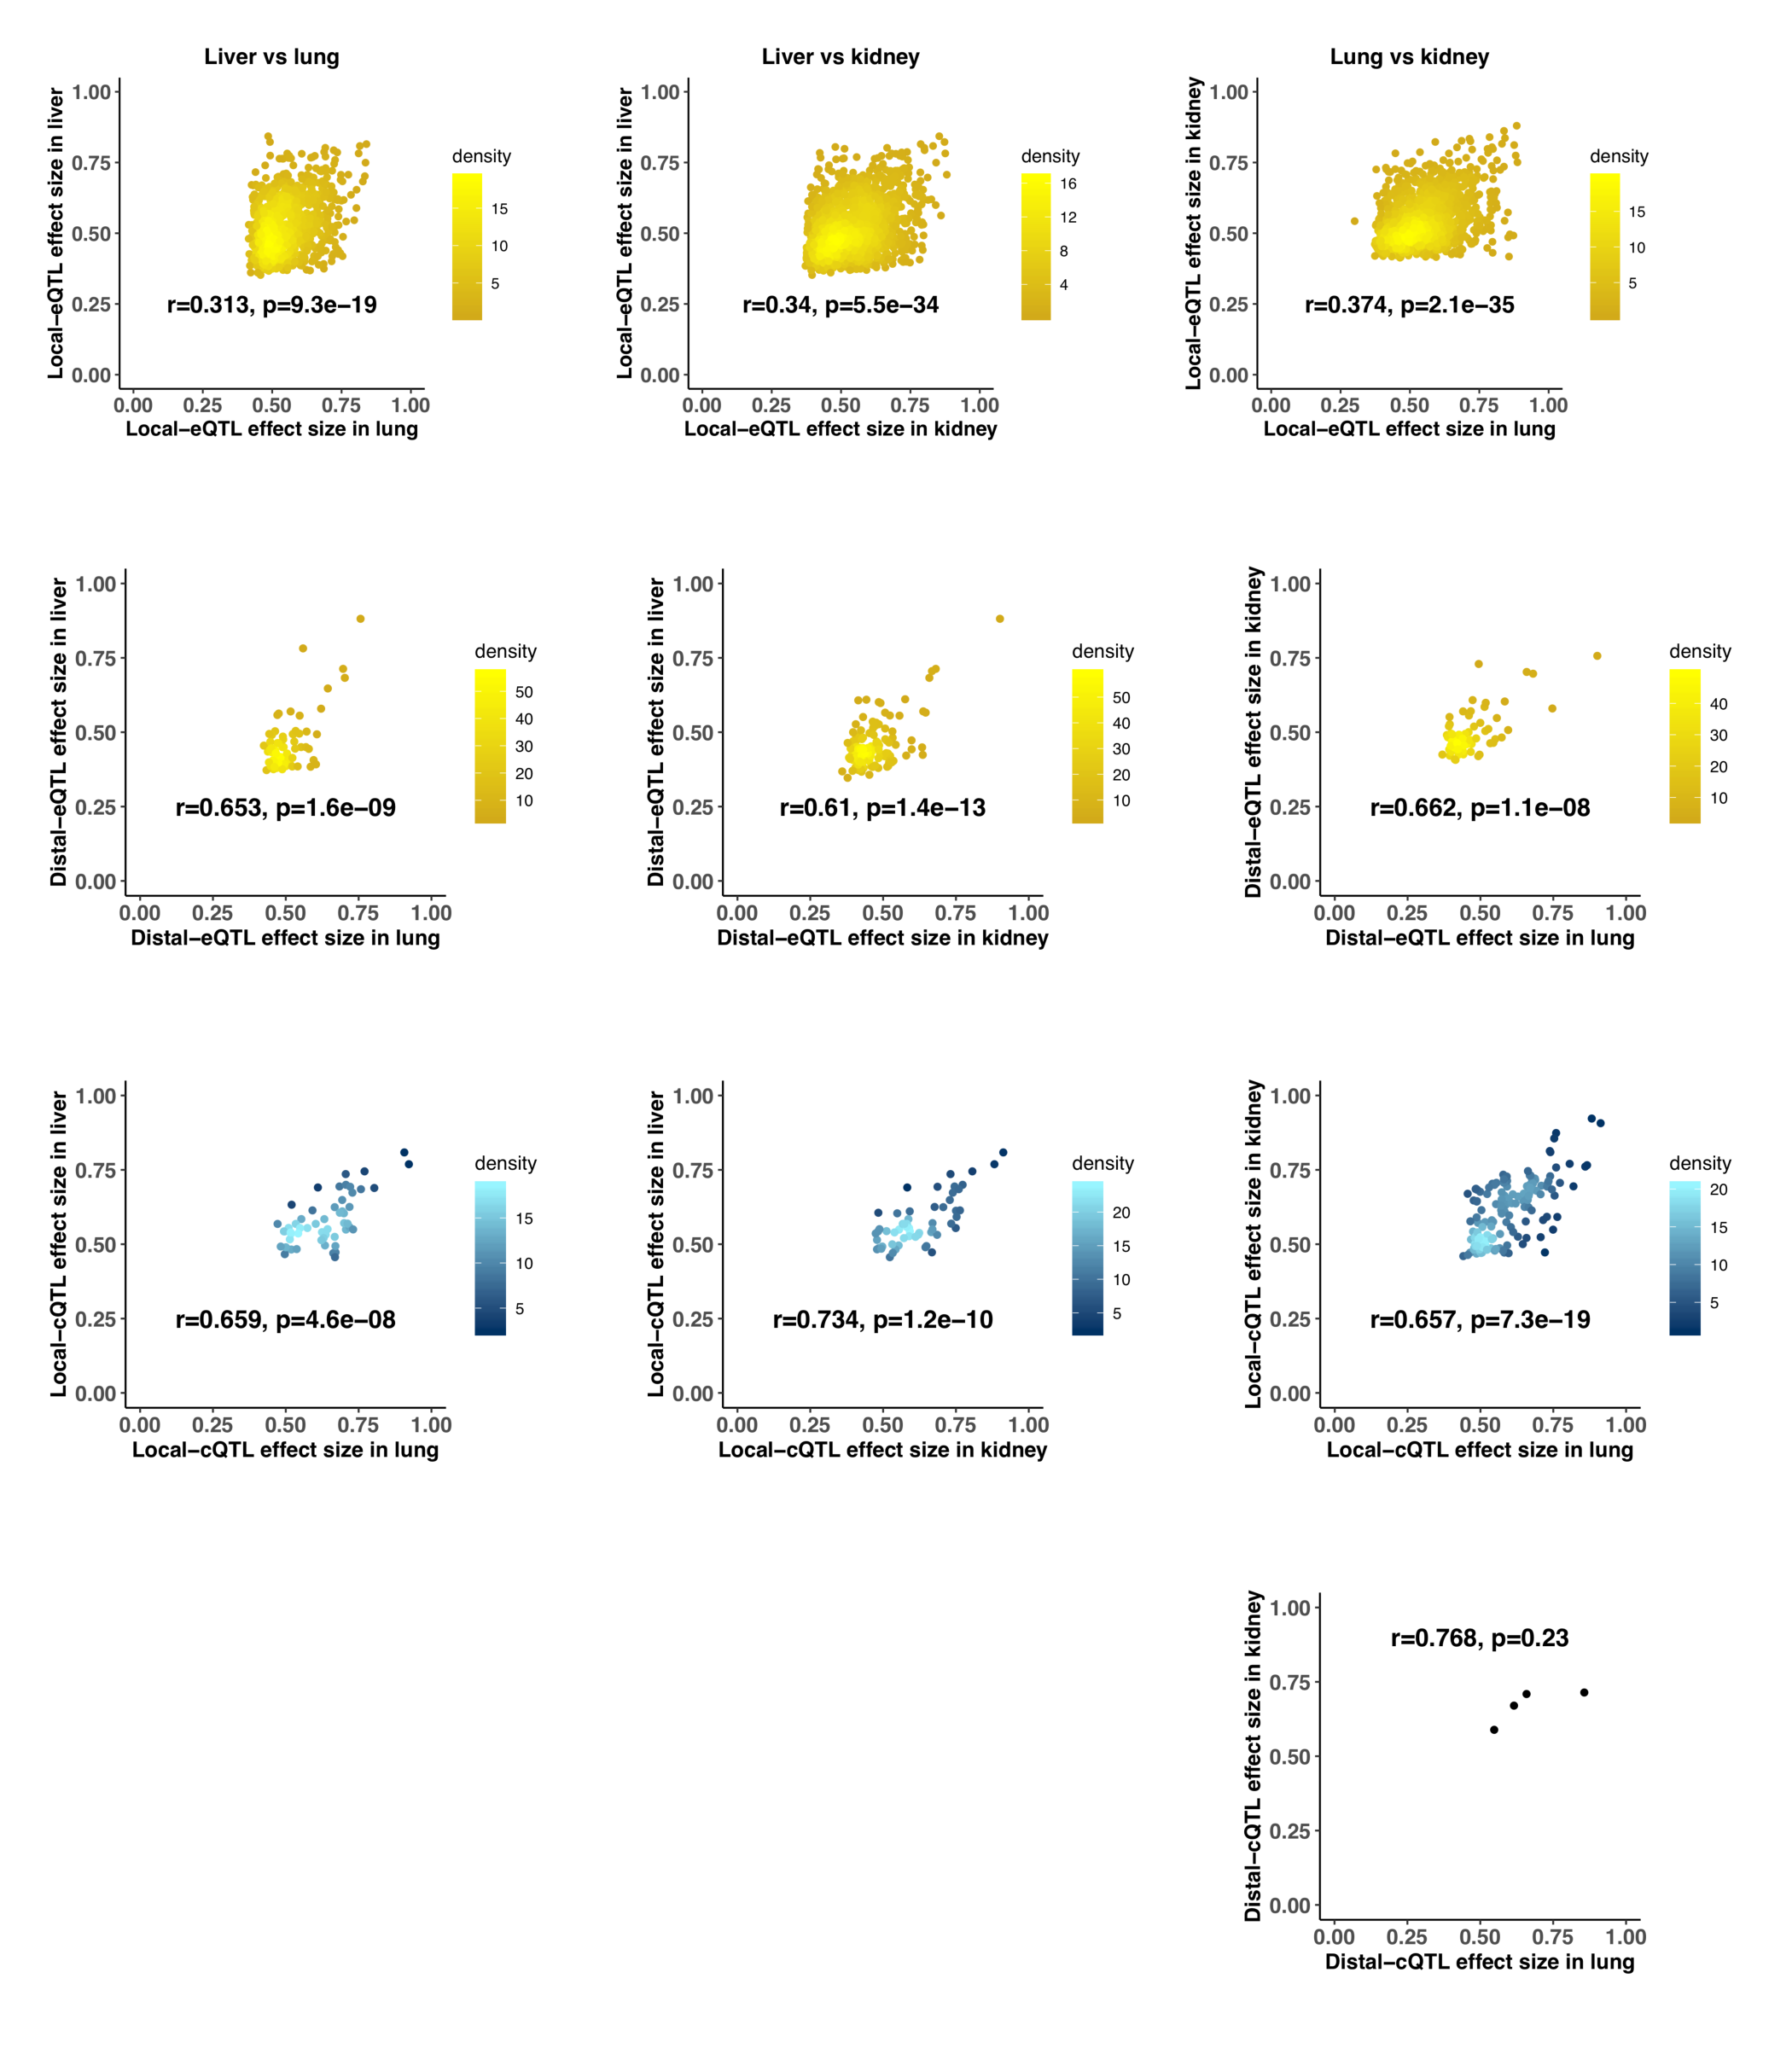
\includegraphics[width=0.9\textwidth, trim={0in 0in 0in 0in}, clip]{figs/effect_size_by_effect_size.pdf}
\caption{\textbf{Effect sizes between QTL pairs are lowly but significantly correlated.} Comparisons of QTL effects sizes, calculated according to Eq \ref{eq:effect_size}, between (liver/lung) are in the left column, (liver/kidney) middle column, and (lung/kidney) right column. eQTL are yellow and cQTL are blue. Local-eQTL are plotted in the top row, distal-eQTL in the second row, local-cQTL in the third row, and distal-cQTL in the bottom row, with only four pairs detected in (lung/kidney). 
\label{fig:qtl_effect_size_comparison}}
\end{figure*}

\begin{figure*}[hp]
\renewcommand{\familydefault}{\sfdefault}\normalfont
\centering
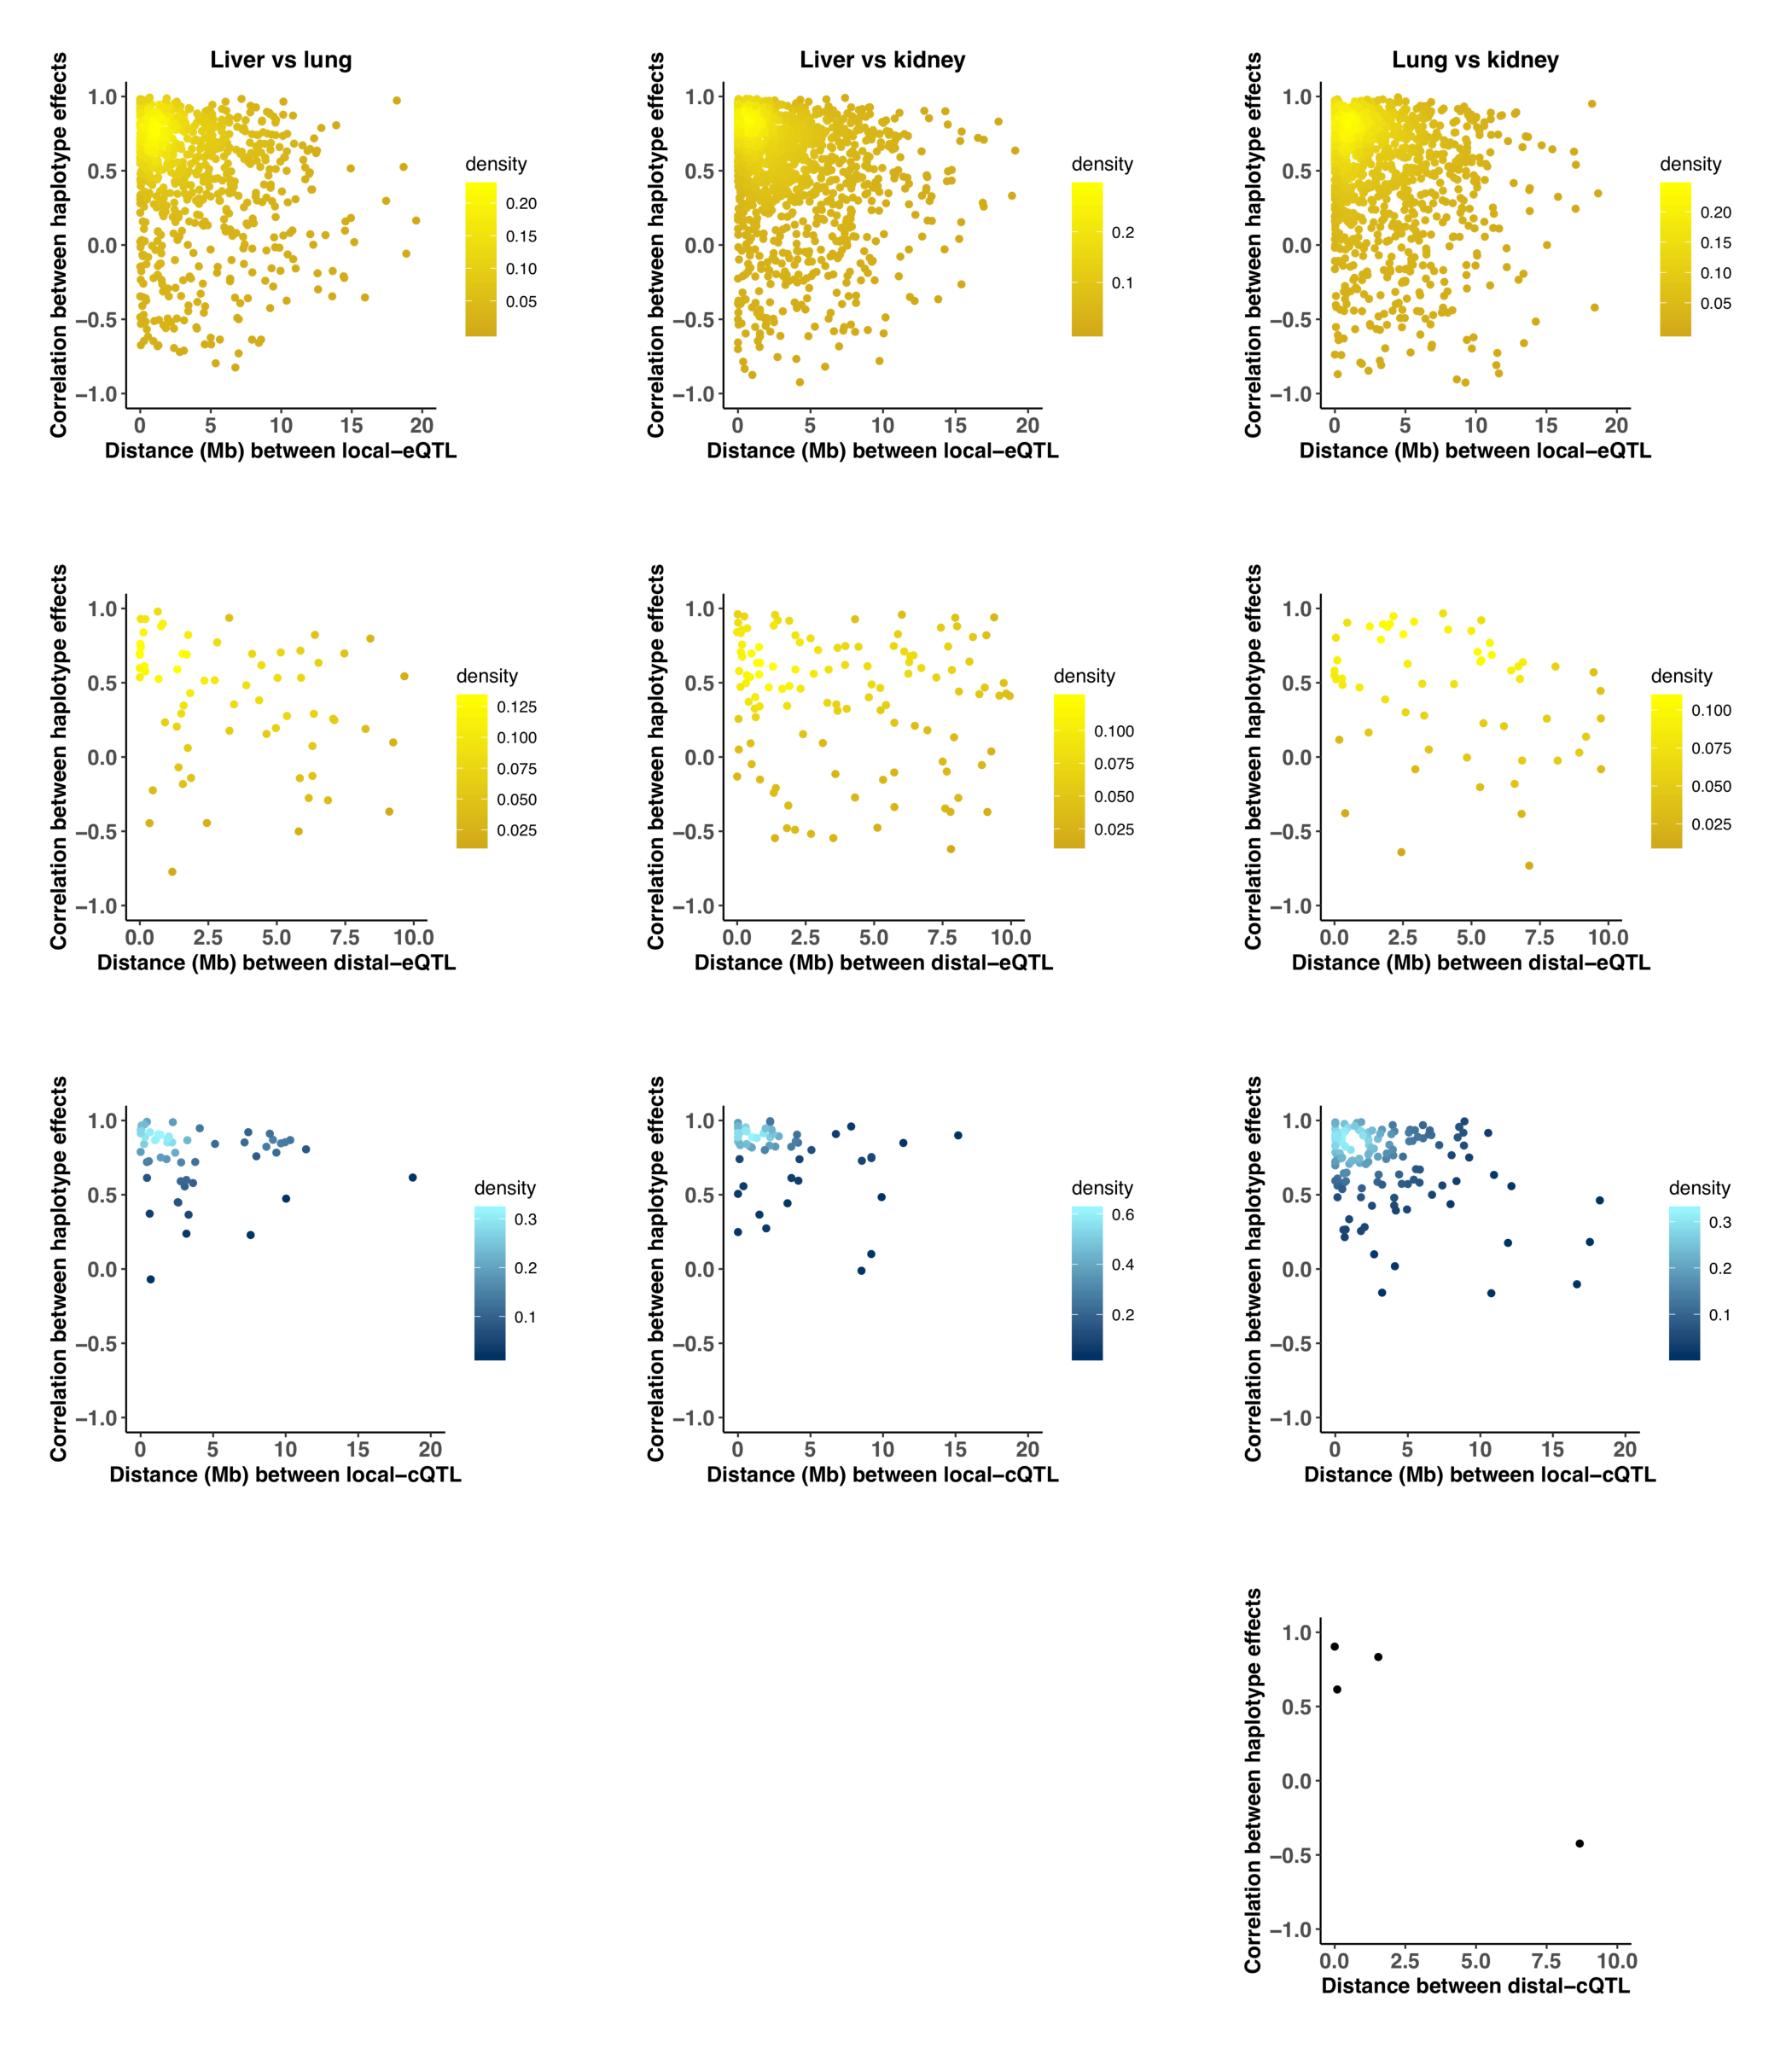
\includegraphics[width=0.9\textwidth, trim={0in 0in 0in 0in}, clip]{figs/effect_size_cor_by_dist.pdf}
\caption{\textbf{QTL pairs with highly correlated founder haplotype effects map proximally to each other.} Founder effects were estimated as constrain BLUPs. Pairwise correlations of the 8-element effect vectors were calculated for QTL pairs, and plotted again the distance between the QTL coordinates inMb for (liver/lung) in the left column, (liver/kidney) in the middle column, and (lung/kidney) in the right column. Single eQTL and cQTL pairs are represented as a yellow and blue dots, respectively. Local-eQTL are shown in the top row, distal-eQTL in the second row, local-cQTL in the third row, and distal c-QTL in the bottom row, for which only four pairs were detected in (lung/kidney).
\label{fig:qtl_cor_by_distance_comparison}}
\end{figure*}

\clearpage

\begin{figure*}[hp]
\renewcommand{\familydefault}{\sfdefault}\normalfont
\centering
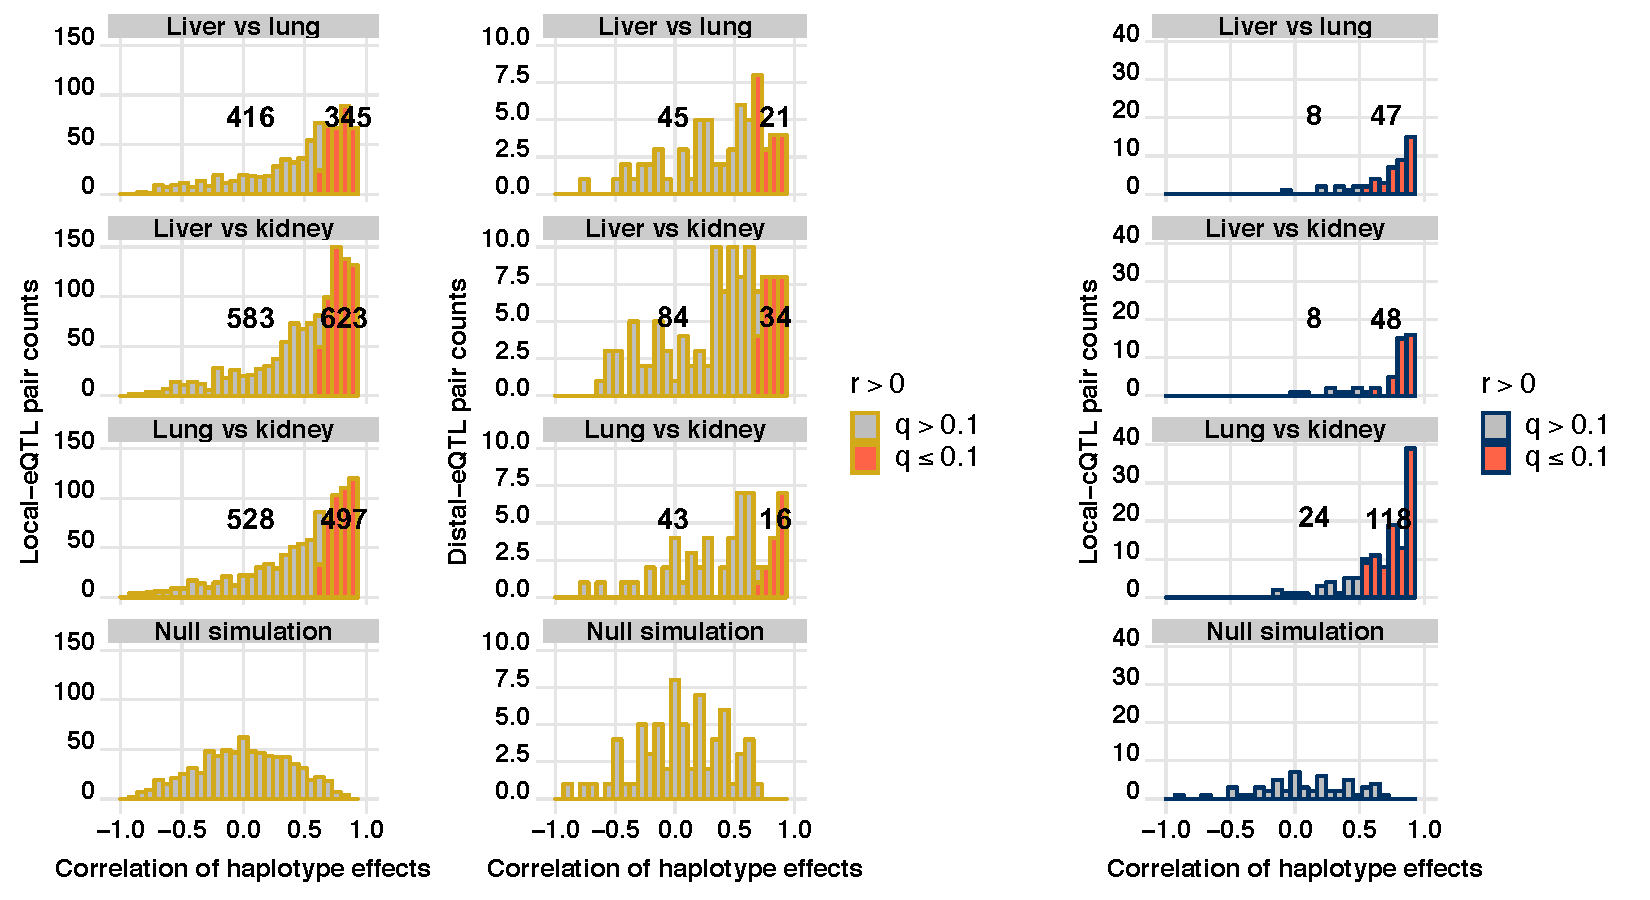
\includegraphics[width=\textwidth, trim={0in 0in 0in 0in}, clip]{figs/qtl_pair_cor_histograms.pdf}
\caption{\textbf{Consistent genetic regulation of gene expression and chromatin accessibility observed across tissues.} Enrichment of significantly correlated founder haplotype effects detected in QTL pairs for gene expression and chromatin accessibility. Pairs of QTL observed in multiple tissues were defined for local-eQTL (left column), distal-eQTL (middle column), and local-cQTL (right column). Only four pairs of distal-cQTL were observed, all shared between lung and kidney. A right-tailed test the correlation between founders effects ($H_{A}: r > 0$) was performed for each QTL pair, producing $p$-values that were then FDR adjusted. Null simulations of uncorrelated 8-element vector pairs for each class of QTL and pairwise tissue comparison emphasize the observed enrichment in correlated founder effects between QTL pairs.  
\label{fig:qtl_pair_histograms}}
\end{figure*}

\begin{figure*}[hp]
\renewcommand{\familydefault}{\sfdefault}\normalfont
\centering
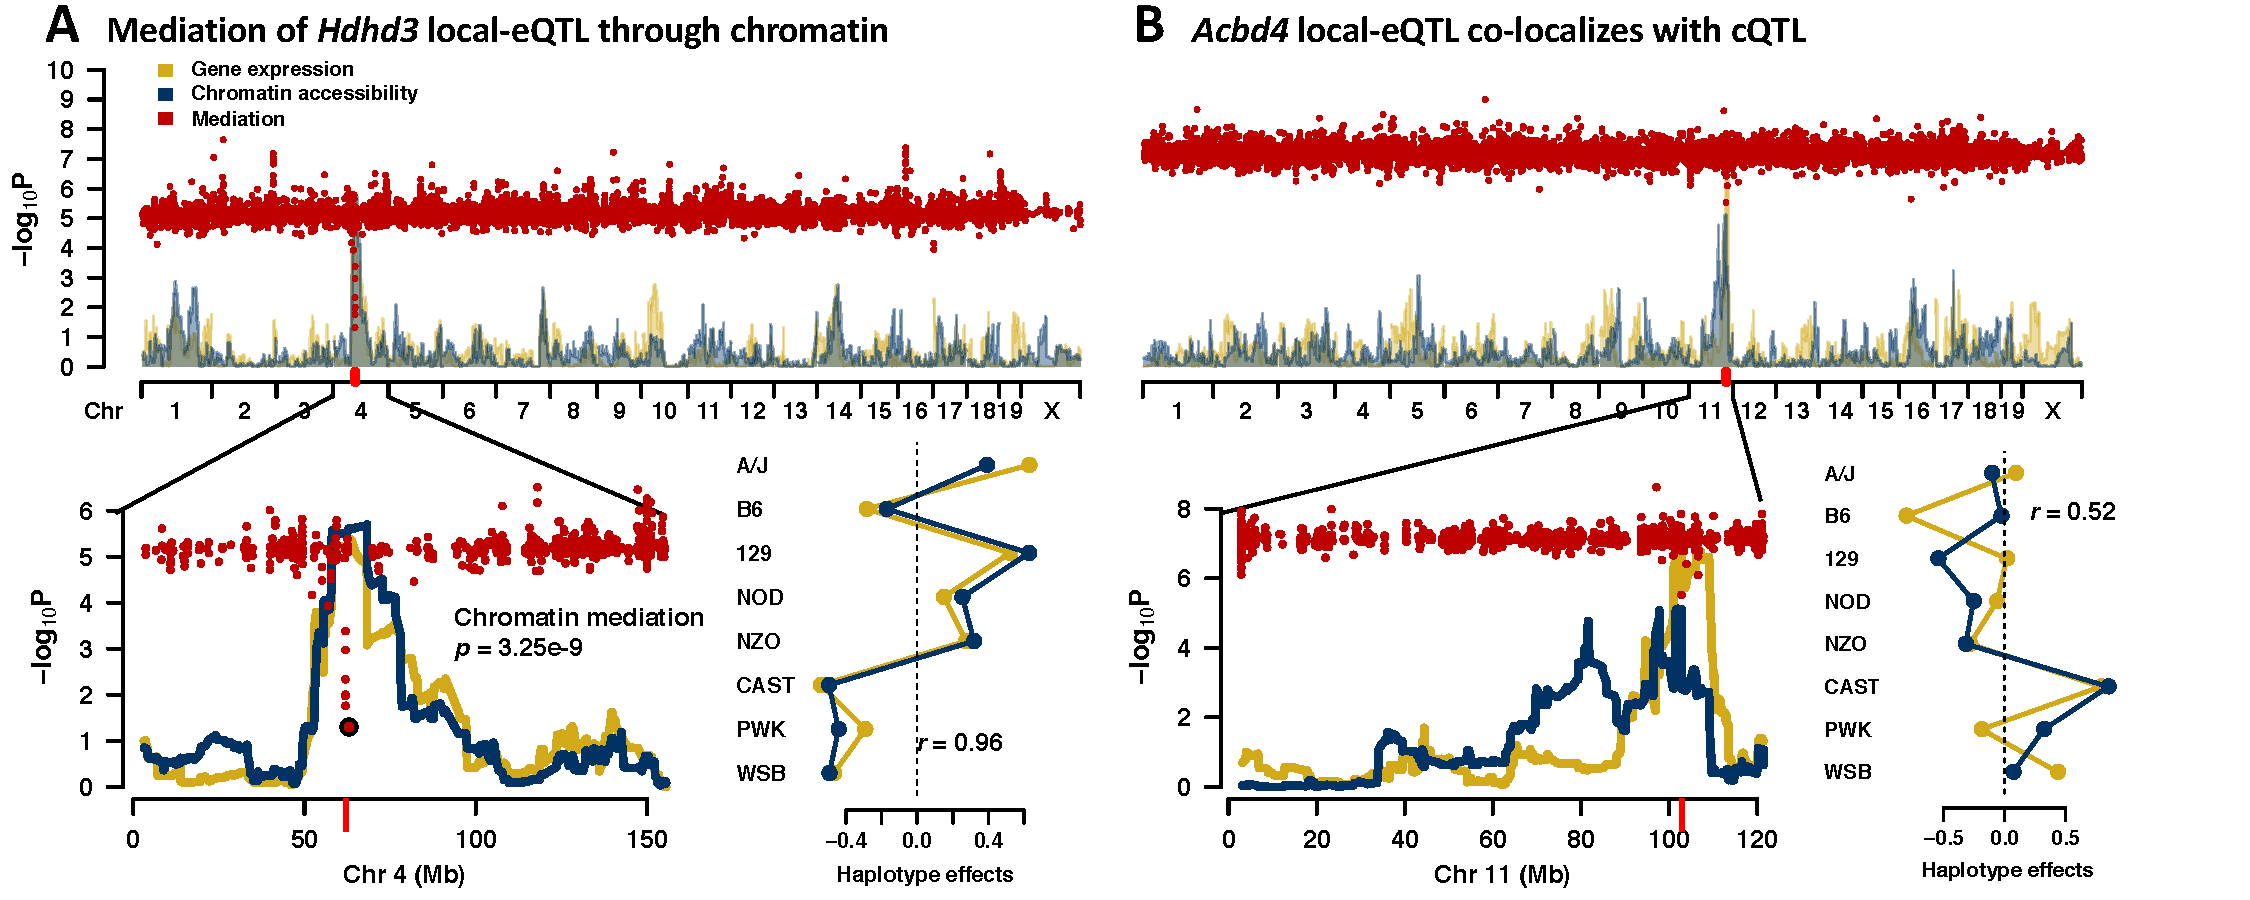
\includegraphics[width=\textwidth]{figs/mediation_or_colocal.pdf}
\caption{\textbf{Co-localizing eQTL and cQTL are not sufficient for statistical mediation.} The approach used to detect mediation through chromatin accessibility requires that the eQTL and cQTL co-localize (both within 10Mb of the gene TSS), as well as possess similar founder haplotype effect patterns. Co-localizing cQTL are observed for local-eQTL for both \textit{Hdhd3} in liver (A) and \textit{Acbd4} in kidney (B). QTL and mediation scans are included \textbf{[top]}, with chromosomes 4 and 11 blown up for \textit{Hdhd3} and \textit{Acbd4}, respectively. The red ticks denote the TSS for both genes. The founders effects were estimated as centered and scaled BLUPs. The founder effects for the eQTL and cQTL are highly correlated ($r = 0.96$) for \textit{Hdhd3}, but not for \textit{Acbd4} ($r = 0.52$). Strong mediation of the \textit{Hdhd3} eQTL through chromatin is detected, but not for \textit{Acbd4}. The effect size of the proximal cQTL to \textit{Acbd4} is smaller than its eQTL, also inconsistent with the relationship depicted in \textbf{Figure \ref{fig:graph} [top]}.
\label{fig:colocalization}}
\end{figure*}

\begin{figure*}[hp]
\renewcommand{\familydefault}{\sfdefault}\normalfont
\centering
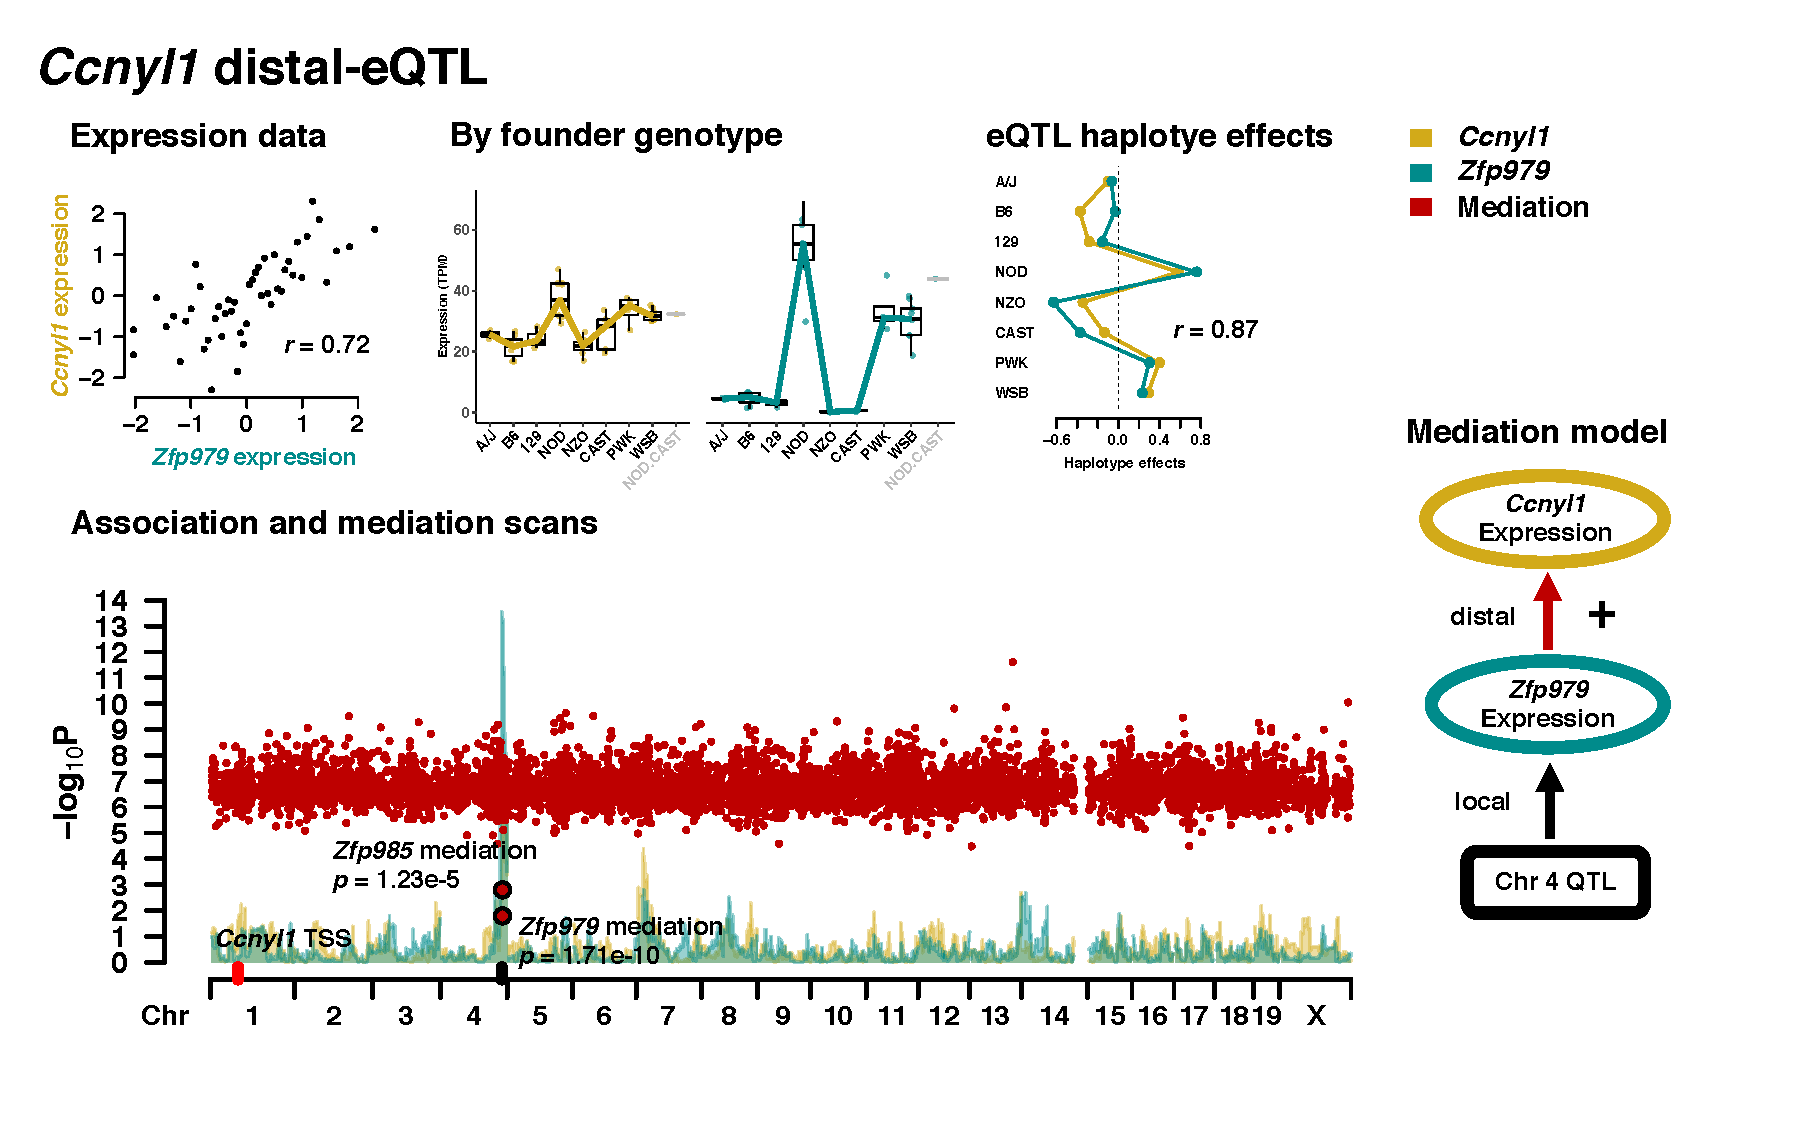
\includegraphics[width=\textwidth, trim={0in 0.5in 0in 0in}, clip]{figs/ccnyl1_mediation.pdf}
\caption{\textbf{Mediation of \textit{Ccnyl1} distal-eQTL through \textit{Zfp979} expression.} Expression of \textit{Ccnyl1} and \textit{Zfp979} are correlated ($r = 0.72$) in lung, which is also observed in the expression data categorized by diplotype and the founder effects estimated as scaled BLUPs. The distal-eQTL on chromosome 4 for \textit{Ccnyl1} corresponds closely to local-eQTL of \textit{Zfp979}. \textit{Ccnyl1} is located on chromosome 1, indicated by the red tick. \textit{Zfp979} and \textit{Zfp985}, both zinc finger proteins likely with DNA binding properties, are identified as strong candidate mediators of the distal-eQTL at genome-wide significance. The correlations, magnitude of effects, and mediation are consistent with the simple relationship depicted in the graph on the \textbf{[right]}. The distal-eQTL and candidate mediators are located in the same region of interest defined in \cite{HamiltonWilliams2013}, which also regulates \textit{Akr1e1} expression. 
\label{fig:ccnyl1_exmediation}}
\end{figure*}

\clearpage

\begin{figure*}[hp]
\renewcommand{\familydefault}{\sfdefault}\normalfont
\centering
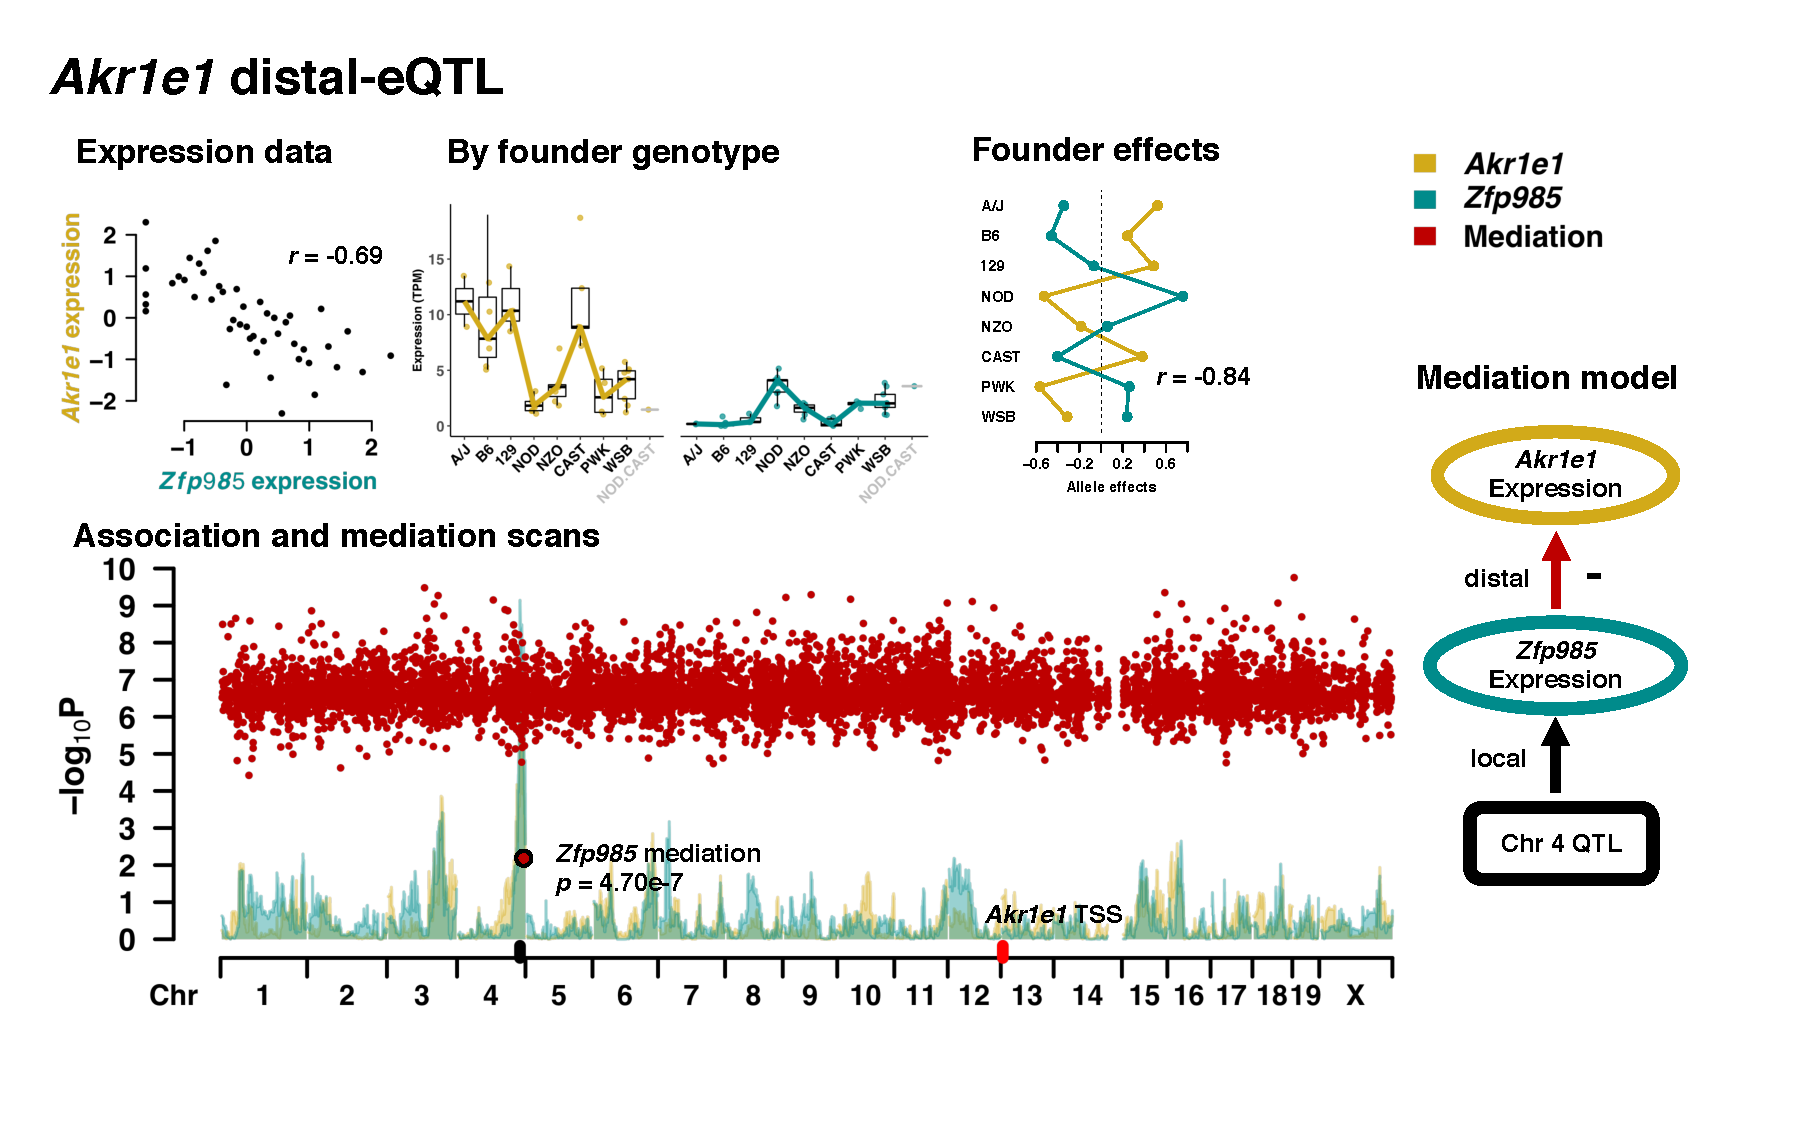
\includegraphics[width=\textwidth, trim={0in 0.5in 0in 0in}, clip]{figs/akr1e1_mediation.pdf}
\caption{\textbf{Mediation of \textit{Akr1e1} distal-eQTL through \textit{Zfp985} expression.} Expression of \textit{Akr1e1} and \textit{Zfp985} are anti-correlated ($r = -0.69$) in lung. This relationship is also observed in the expression data plotted as boxplots, categorized by most likely diplotype, and the founder haplotype effects, estimated as scaled BLUPs. The QTL and mediation scans reveal that \textit{Akr1e1}, TSS marked with a red tick on chromosome 13, possesses a distal-eQTL on chromosome 4 that is proximal to the strong local-eQTL of \textit{Zfp985}. The mediation scan identifies \textit{Zfp985} as a strong candidate mediator consistent with the mediation model included on the \textbf{[right]}. A more complete picture of the genetic regulation of \textit{Akr1e1} expression is pieced together by looking across all three tissues and includes a potential chromatin mediator (\textbf{Figure \ref{fig:akr1e1_full_model.pdf}}).
\label{fig:akr1e1_exmediation}}
\end{figure*}

\begin{figure*}[hp]
\renewcommand{\familydefault}{\sfdefault}\normalfont
\centering
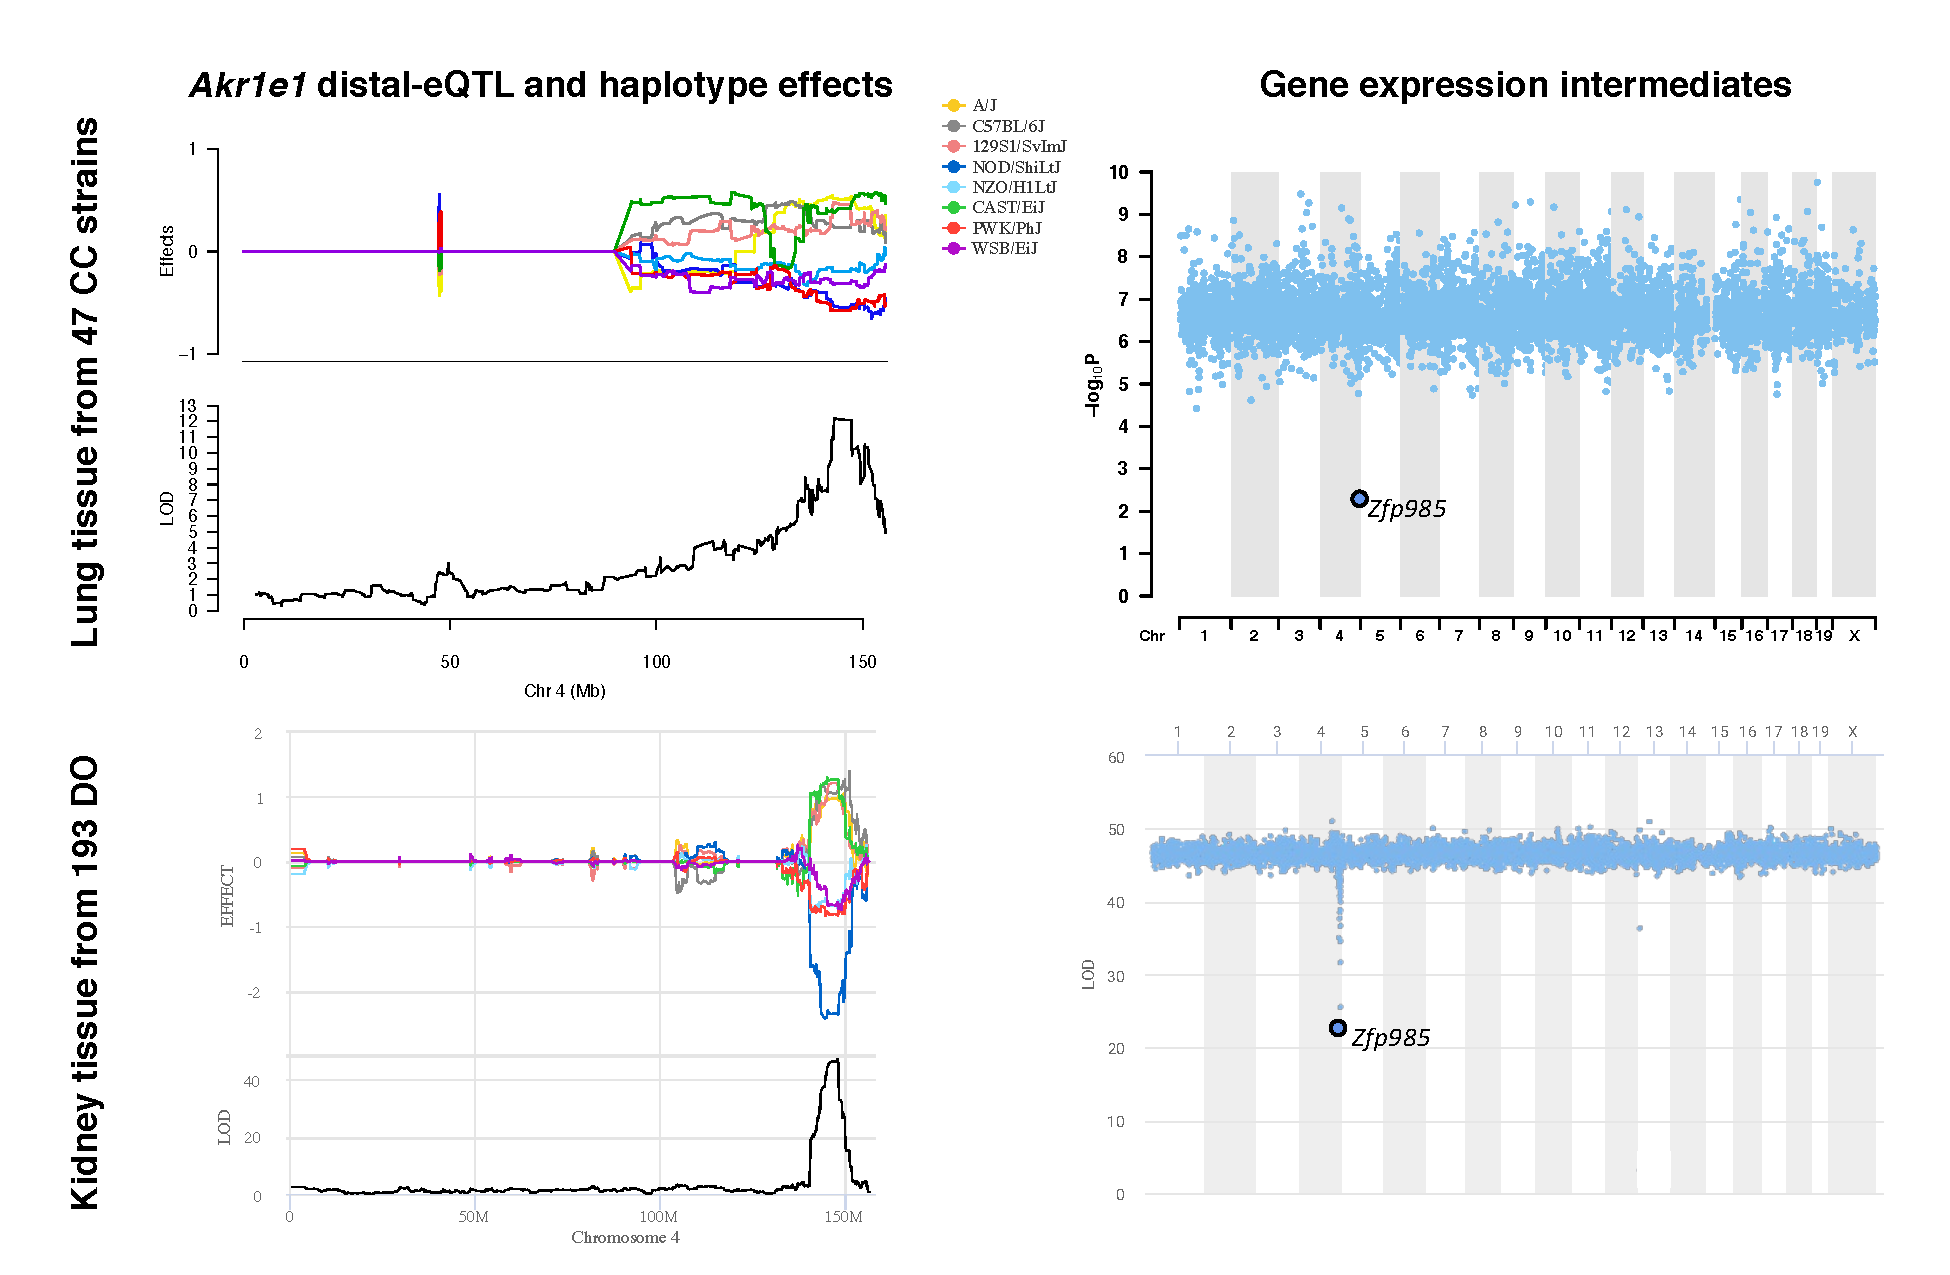
\includegraphics[width=\textwidth, trim={0in 0in 0in 0in}, clip]{figs/do_confirmation_akr1e1.pdf}
\caption{\textbf{Confirmation of \textit{Akr1e1} distal-eQTL and mediation by \textit{Zfp985} in kidney tissue of Diversity Outbred mice.} A genome-wide significant distal-eQTL was detected for \textit{Akr1e1} in liver, lung (shown here), and kidney tissues from 47 CC strains. In a larger sample of kidney tissue from outbred DO mice, the same distal-eQTL and mediation relationship were observed. As expected, the larger sample results in greater statistical significance, and confirms that the NOD effect is more strongly negative than NZO, PWK, and WSB, which the effects plots the \textit{Zfp985} local-eQTL suggested. Notably, \textit{Zfp985} was not tested in the CC kidney because of low levels, though the distal-eQTL for \textit{Akr1e1} is consistent with its activity, which is here confirmed in the DO.
\label{fig:do_akr1e1}}
\end{figure*}


\begin{figure*}[hp]
\renewcommand{\familydefault}{\sfdefault}\normalfont
\centering
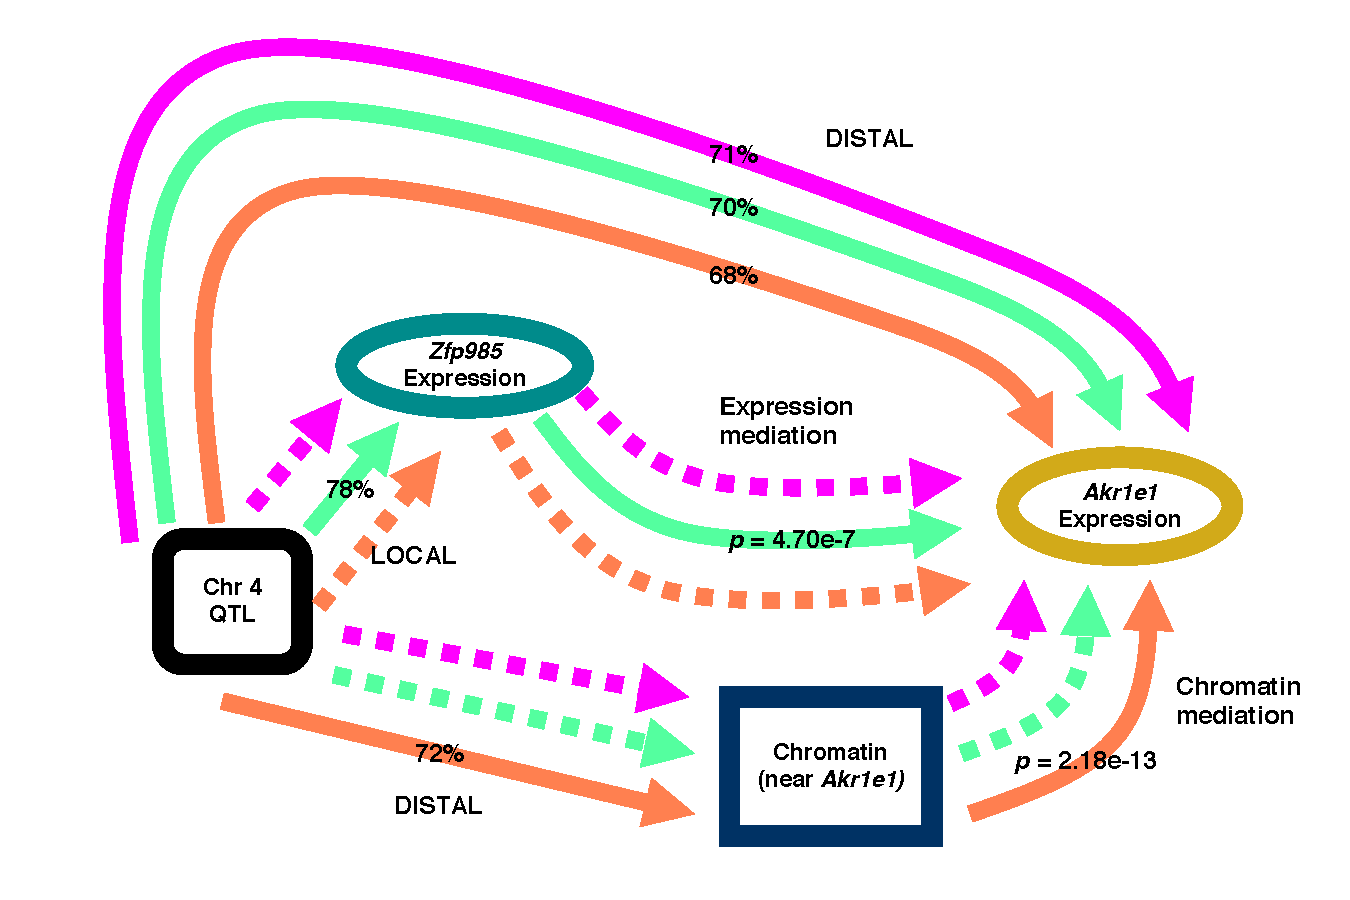
\includegraphics[width=\textwidth, trim={0in 0in 0in 0in}, clip]{figs/akr1e1_observed_relationships.pdf}
\caption{\textbf{Observed relationships across the three tissues related to the genetic regulation of \textit{Akr1e1} expression.} The model for the distal genetic regulation of \textit{Akr1e1} expression, described in \textbf{Figure \ref{fig:akr1e1_full_model}}, was reconstructed from these observed relationships. Solid arrows were observed, whereas dashed arrows are assumed. Effect sizes represent the proportion of variance explained by the QTL and mediation $p$-values (permP) were defined using a permutation procedure. The assumed relationships are supported by the presence of the distal-eQTL in all three tissues. The \textit{Zfp985} mediator relationship in kidney, though not observed in the CC, was observed in the related DO population.
\label{fig:akr1e1_relationships}}
\end{figure*}

\end{document}
